% =================================================================================
% THESIS LM V.0.2: 15-Aug-2026 - Updated results
% =================================================================================
% 01-May-2026: V.1.0 - PRISM. Reviewed and corrected - Finalized as baseline.
% 03-May-2026: V.1.5 - Ablation Study added!!!
% 06-May-2026: V.1.6 - Ablation Study integrated in mainstream content
% 07-May-2026: V.1.6 - \citep{Siraskar2023SLR}
% 21-May-2026: V.1.84/1.85 -- Added tool wear decision image
% 22-May-2026: V.1.86 -- Added RL and AM tables in section 5. Architecures 
% 24-May-2026: V.1.90 -- Expanded SLR using UnderMind
% 24-May-2026: V.1.90 -- Refactored tables
% 15-Aug-2026: V.LM.0 -- Independence Day - Important Results and Conclusions Updates  
% =================================================================================

\documentclass[12pt,oneside]{book}
\usepackage[utf8]{inputenc}
\usepackage{amsfonts}
\usepackage[T1]{fontenc}
\usepackage{lmodern}
\usepackage[dvipsnames]{xcolor}
\usepackage[a4paper, top=1.25in, bottom=1in, left=1.25in, right=1in]{geometry}
% \usepackage[a4paper,margin=1.2in]{geometry}
\usepackage[toc,page]{appendix}
\usepackage{graphicx}
\usepackage{epigraph} 
\usepackage{caption}
\usepackage{subcaption}   % Subfigures
\usepackage{pdfpages}

%% Reference / Citation set-up: Configuration ** BibTex **
\usepackage{natbib}
\setcitestyle{authoryear, open={(},close={)}}

%% Images and Figures
\graphicspath{{./Figures/}{./Figures/A1_Literature_Survey/}{./Figures/A2_REINFORCE_for_PdM/}{./Figures/A3_Nadaraya_Watson_AM_for_PdM/}{./Figures/A4_RL_with_Attention_for_PdM/}}

%% CUSTOM PACKAGES
\usepackage{amsmath,amssymb,amsfonts}%
\usepackage{listings}		% Code listing
\usepackage{algorithm}		% Algorithm
\usepackage[noend]{algpseudocode} 		% Pseudo-code
\usepackage{chronosys} 	% Chronology

\usepackage{array}        % Table spacing
\usepackage{enumitem}     % Enumerate customization
\usepackage{pdflscape}    % Landscape page
\usepackage{booktabs,tabularx}
\usepackage{arydshln} 	% dashed lines in table
\usepackage{longtable}    % Long multi-page tables
\usepackage{lscape}
\usepackage{multirow}
\usepackage{makecell}
\usepackage{setspace}	  % Line spacing when using default layout
\usepackage{xcolor, soul, colortbl} % Highlights
\usepackage{float}        % Fix tables
\usepackage{hyperref}
\hypersetup{colorlinks=true, linkcolor=RoyalBlue, citecolor=RoyalBlue, filecolor=blue, urlcolor=RoyalBlue}
\usepackage{tikz}
\usetikzlibrary{arrows.meta,positioning,fit}

%% Global table row spacing
\renewcommand{\arraystretch}{1.5}

%% MACROS
\newcommand{\hlc}[2][cyan!15]{{\colorlet{foo}{#1} \sethlcolor{foo}\hl{#2}}}
\newcommand{\hlr}{\rowcolor{cyan!10}}
\algnewcommand{\LineComment}[1]{\State \(\triangleright\) #1}
\newcommand{\rowspace}[1]{\renewcommand{\arraystretch}{#1}}
\newcommand{\ltmidrule} {\arrayrulecolor{black!20} \midrule}
\newcommand{\drmidrule} {\arrayrulecolor{black!40} \midrule}

%% From Attention article
% \newcolumntype{C}{>{\centering\arraybackslash}X}
% \newcolumntype{L}{>{\raggedright\arraybackslash}X}
% \newcolumntype{R}{>{\raggedleft\arraybackslash}X}

%% From SLR? or other article
\newcolumntype{L}[1]{>{\raggedright\arraybackslash}p{#1}}
\newcolumntype{R}[1]{>{\raggedleft\arraybackslash}p{#1}}
\newcolumntype{C}[1]{>{\centering\arraybackslash}p{#1}}

\makeatletter
\providecommand\adl@rowsL{}
\providecommand\adl@rowsR{}
\providecommand\adl@colsL{0}
\providecommand\adl@colsR{0}
\makeatother

\definecolor{codegray}{rgb}{0.5,0.5,0.5}
\definecolor{ltgray}{gray}{0.93}
\definecolor{dblue}{rgb}{0.20, 0.30, 1.0}

\makeatletter
\def\SOUL@hlpreamble{%
	\setul{}{2.8ex}% default is 2.5ex
	\let\SOUL@stcolor\SOUL@hlcolor
	\SOUL@stpreamble
}
\makeatother

\begin{document}
\onehalfspacing
\captionsetup[figure]{margin=1.5cm,font=small,labelfont={bf},name={Figure},labelsep=colon,textfont={it}}
\captionsetup[table]{margin=1.5cm,font=small,labelfont={bf},name={Table},labelsep=colon,textfont={it}}
\frontmatter

\begin{titlepage}
	\begin{center}
	{\LARGE Symbiosis International (Deemed University)}\\[0.25cm]
	{\Large Symbiosis Institute of Technology, Pune}\\[1cm]
	\linespread{1.2}\huge {\bfseries Remaining Useful Life Estimation using Deep Reinforcement Learning during Machining}\\[1.5cm]
	\linespread{1}
	{\includegraphics[width=4.5cm]{SIUlogo.PNG}}{\mbox{}}\\[1.2cm]
	{{\Large\textbf{Rajesh Siraskar}}\\{\large PRN 21079001012}}\\[0.2cm]
	\begin{tabular}{>{\centering\arraybackslash}p{0.30\textwidth} >{\centering\arraybackslash}p{0.30\textwidth} >{\centering\arraybackslash}p{0.38\textwidth}}
		\begin{minipage}[t]{\linewidth}\begin{spacing}{0.7}\centering {\large Dr. Satish Kumar}\\{\large Professor}\\{\large Symbiosis Institute of Technology, Pune}\end{spacing}\end{minipage} &
		\begin{minipage}[t]{\linewidth}\begin{spacing}{0.7}\centering {\large Dr. Shruti Patil}\\{\large Director SAAI}\\{\large Symbiosis Artificial Intelligence Institute}\end{spacing}\end{minipage} &
		\begin{minipage}[t]{\linewidth}\begin{spacing}{0.7}\centering {\large Dr. Ambarish Kulkarni}\\{\large Associate Professor}\\{\large Swinburne University of Technology, Australia}\end{spacing}\end{minipage} 
	\end{tabular}\\[0.5cm]
	\vspace{\fill}
	\large A thesis submitted in partial fulfilment of the University's requirements for the degree of Doctor of Philosophy\\[0.6cm]
	August 2026
\end{center}

\end{titlepage}

% -------------------------------------------------------------------
% Declaration
% -------------------------------------------------------------------

\newpage
\section*{\Large Declaration}

All sentences or passages quoted in this thesis from other people's work have been specifically acknowledged through clear cross-referencing to the author, work, and page(s). Any illustrations that are not the author's own have been used with the explicit permission of the originator and are specifically acknowledged. I understand that failure to do so amounts to plagiarism and may be considered grounds for failure.\\[1cm]

\noindent Name:\\[1mm]
\rule[1em]{25em}{0.5pt}

\noindent Signature:\\[1mm]
\rule[1em]{25em}{0.5pt}

\noindent Date:\\[1mm]
\rule[1em]{25em}{0.5pt}

% \includepdf[pages=-]{forms/form.pdf}

% \input{Article_Text/Acknowledgements.tex}

% -------------------------------------------------------------------
% Abstract
% -------------------------------------------------------------------

\chapter*{Research Synopsis}
% \begin{figure}[ht]
% 	\centering
% 	\includegraphics[width=\textwidth, height=\textheight, keepaspectratio]{Synopsis.png}
% 	\caption*{}
% \end{figure}

\begin{enumerate}[leftmargin=*]
    \item We frame milling-tool replacement as a sequential decision problem for predictive maintenance (PdM), rather than only as a remaining-useful-life prediction task.
    \item A schema-adaptive reinforcement learning (RL) environment is developed to compare \textsc{REINFORCE}, DQN, A2C, and PPO across two divergent data schemas -- public IEEE PHM~2010 and primary data generated at Symbiosis Institute of Technology (SIT).
	\item The study evaluates compact observation encoders based on Nadaraya--Watson, temporal, multi-head, and self-attention mechanisms against baselines without attention mechanisms.
	\item Experimental results identify \textsc{REINFORCE} with Nadaraya--Watson attention as the strongest configuration for our in-house Symbiosis Institute of Technology (SIT) university milling schema ($S\approx0.865$), while on IEEE, \textsc{REINFORCE} with self-attention emerges as the clear leader ($S\approx0.886$), both outperforming the best \textsc{PPO} configurations on their respective schemas.
	\item Ablation findings show that attention is beneficial only under specific algorithm--schema combinations, making empirical encoder selection essential rather than automatic.
    \item An architectural taxonomy separating temporal-difference learners from direct policy optimizers offers a plausible mechanistic explanation for why attention helps some algorithms and destabilizes others.
    \item The thesis contributes a reproducible, AutoRL workflow for RL-driven PdM that links maintenance decision design, schema-aware observation handling, compact policy learning, and a maintenance-grounded $\lambda$ metric evaluation.
    \item Four research publications, with one in review, are our contribution to the industrial and scientific community. 
\end{enumerate}

\chapter*{Abstract}

The advent of Industry~4.0 has made data-driven decision-making a cornerstone of modern manufacturing. Predictive maintenance (PdM) sits at the center of this paradigm, shifting maintenance away from costly reactive repairs and inefficient fixed schedules toward proactive, condition-based intervention. Among manufacturing processes, industrial milling presents a demanding maintenance problem because tool wear evolves continuously under stochastic operating conditions. Replacing a cutting tool too early wastes usable tool life, whereas replacing it too late increases the risk of machine damage, rejected parts, and unplanned downtime.

Our research is directed primarily toward the industrial practitioners. We investigate whether reinforcement learning (RL) can produce practical tool-replacement policies for industrial milling equipment. A trained reinforcement learning agent learns to estimate the remaining useful life of the tool during the machining operation, online, and then predict the maintenance action. 

The literature review shows that RL-for-PdM is now an established research direction, but important gaps remain in lightweight policy learning, schema-aware observation design, reproducible model-selection workflows, and maintenance-grounded evaluation. The thesis therefore treats milling-tool replacement not only as a prediction task, but as a sequential decision problem under partial observability.

The work develops a schema-adaptive RL environment for milling-tool PdM, compares \textsc{REINFORCE} with DQN, A2C, and PPO, and evaluates Nadaraya--Watson, temporal, multi-head, and self-attention mechanisms as compact observation encoders. The experimental programme is deliberately staged: preliminary experiments test policy learning across 15 milling-tool environment variants, while the final study evaluates schema-adaptive policies on held-out files from the public IEEE PHM~2010 milling benchmark and an in-house Symbiosis Institute of Technology (SIT) university milling schema. Policy quality is measured using replacement classification metrics in the preliminary study and, in the final study, a metric designed for industrial practitioners -- composite score $S$ that combines tool-life usage, replacement timing $\lambda$, and threshold-violation behavior.

As an outcome of our research we created an AutoRL workbench for industrial practitioners. The workbench helps run automated training pipelines across the multiple algorithms and attention mechanisms, relieving the practitioners from complex hyperparameter tuning and, run automatic evaluations, identifying the best models to use.

The preliminary research was conducted on untuned RL algorithms. The evidence shows that lightweight policy-gradient learning algorithm is not merely a weak baseline. Across all 15 environment variants, \textsc{REINFORCE} achieved the strongest mean precision (0.687), recall (0.629), F1-score (0.609), and the tool-replacement precision-weighted $F_{\beta=0.5}$ score (0.631). Under a best-of-repeated-rounds AutoRL selection view, its mean precision and recall both increased to 0.884, with F1-score of 0.873 and $F_{\beta=0.5}$ of 0.876. These results motivated retaining \textsc{REINFORCE} as a first-class lightweight candidate in the final schema-adaptive evaluation rather than treating it only as a simple reference model.

The final research work was based on tuned RL algorithms augmented with attention encoders, using the AutoRL workbench. On the richer SIT schema, the strongest configuration was \textsc{REINFORCE} with Nadaraya--Watson attention, achieving a mean evaluation score of $0.8646$ ($\pm0.2032$ std. dev.); the strongest \textsc{PPO} configuration on SIT used multi-head attention ($0.8004 \pm 0.2694$). On IEEE, the leading configuration was \textsc{REINFORCE} with self-attention ($0.8860 \pm 0.0708$), with the strongest \textsc{PPO} configuration using Nadaraya--Watson attention ($0.8343 \pm 0.1867$). Without attention, \textsc{PPO} provided the strongest baseline in both schemas (SIT: $0.6313$; IEEE: $0.7484$), but one-tailed Welch tests show \textsc{REINFORCE} significantly exceeds \textsc{PPO} once attention is included (SIT: $t=3.1941$, $p=0.0007$; IEEE: $t=1.9865$, $p=0.0243$), whereas no such advantage exists at baseline ($p>0.90$ in both schemas).

The ablation results show why the thesis treats attention as an empirical design choice rather than as an assumed improvement. On SIT, attention improved the pooled all-algorithm mean score from $0.4033$ to $0.4830$ ($t=4.6626$, $p=0.0000$), and for \textsc{REINFORCE} specifically, attention increased the mean score from a no-attention baseline of $0.4907$ to $0.7492$ ($t=7.1139$, $p=0.0000$), peaking at $0.8646$ with Nadaraya--Watson. On IEEE, however, pooled attention across all four algorithms did \emph{not} improve on the no-attention baseline -- the mean score fell from $0.6589$ to $0.5906$ ($t=-2.2584$, $p=0.9873$), an ``algorithm masking effect'' driven by severe degradation in \textsc{DQN} and \textsc{A2C}. Attention became reliably beneficial on IEEE only once the comparison was restricted to the stronger policy-gradient learners (\textsc{PPO} and \textsc{REINFORCE}), where the pooled mean score increased from $0.7090$ to $0.8313$ ($t=3.7724$, $p=0.0002$). Exploring mechanism-level effects, Multi-Head Attention proved to be the most universally robust encoder mechanism across representations. The learned policies also remained compact: average serialized \textsc{REINFORCE} policy size was approximately 169~kB on both schemas. A plausible mechanistic explanation follows from an architectural taxonomy that separates temporal-difference learners (\textsc{DQN}, \textsc{A2C}), whose bootstrapped value targets are destabilized by shifting attention-derived features, from direct policy optimizers (\textsc{REINFORCE}, \textsc{PPO}), whose Monte-Carlo returns or trust-region updates tolerate -- and exploit -- the same representational shift.

Overall, the thesis shows that carefully designed lightweight RL can support practical milling-tool replacement decisions, but only when the algorithm, observation encoder, sensor schema, and maintenance-grounded metric are selected together. Its central contribution is therefore a reproducible, workflow for RL-driven PdM: define the maintenance decision, instantiate a schema-adaptive environment, compare compact and deeper learners, include no-attention as a first-class baseline, and select the final policy using quantitative metrics tied directly to tool usage, timing quality, and threshold safety.

% -------------------------------------------------------------------
% ToC and list of figures, tables
% -------------------------------------------------------------------
\tableofcontents
\listoffigures
\listoftables

% -------------------------------------------------------------------
% Main sections (as required)
% -------------------------------------------------------------------
\mainmatter
\onehalfspacing

% -------------------------------------------------------------------
% Chapter 1: Introduction (primarily based on SLR)
% -------------------------------------------------------------------

\chapter{Introduction}\label{ch:introduction}

\section{Introduction and Background}

\subsection{Significance of Research}

Industry~4.0 is increasingly grounded in connected sensing, embedded intelligence, and distributed computation. Recent industry estimates indicate that the number of connected IoT devices reached 18.5~billion in 2024 and is projected to rise to 21.1~billion by the end of 2025, with continued expansion toward 39~billion by 2030 \citep{IoTAnalytics2025}. In manufacturing, this expanding sensor base enables continuous equipment monitoring, richer machine-state estimation, and tighter feedback loops between the physical shop floor and digital decision systems. In this broader transformation, the smart factory is commonly understood as a connected and flexible production system that uses operational data to learn and adapt to changing conditions \citep{Deloitte2025Survey}.

%% \citep{DeloittePdM} - replace with 2025 Survey below for 5-20 percent effect

The business case for such transformation is now concrete rather than speculative. Deloitte's 2025 smart manufacturing survey reports that manufacturers are seeing average net improvements of 10--20\% in production output, 7--20\% in employee productivity, and 10--15\% in unlocked capacity from smart-manufacturing initiatives \citep{Deloitte2025Survey}. At the same time, maintenance remains a major operational and financial lever: Deloitte reports that poor maintenance strategies can reduce plant productive capacity by 5--20\% \citep{Deloitte2025Survey}. This is especially relevant in general manufacturing environments and for machine tools such as milling machines, where a single asset's degradation can propagate into queueing delays, lost spindle time, missed delivery schedules, and reduced overall equipment effectiveness.

Within this setting, predictive maintenance (PdM) is one of the most commercially significant Industry~4.0 applications. Its importance is amplified by the high cost of unplanned downtime. Siemens reports that, in 2024, unplanned downtime cost the world's 500 largest companies 11\% of their revenues, totaling approximately USD~1.4~trillion \citep{SiemensDowntime2024}. For production-intensive sectors, the cost of even a single lost hour can be extremely large \citep{SiemensDowntime2024}. These figures make clear that maintenance is not merely a technical support function; it is a direct determinant of profitability, resilience, and production continuity.

This is where reinforcement learning (RL) becomes significant. Predictive maintenance is not only a forecasting problem; it is also a sequential decision problem under uncertainty. In practice, maintenance decisions must balance short-term production objectives against long-term degradation, failure risk, maintenance cost, and the consequences of unnecessary intervention. For milling machines and related manufacturing assets, RL offers a principled framework for learning policies that decide when to continue operation, inspect, slow down, or intervene, based on observed machine condition and operating context. This gives RL particular relevance where static maintenance thresholds or fixed schedules are too rigid to capture changing workloads and degradation patterns.

The significance of this research is strengthened further by the rise of edge computing. IDC estimates that global spending on edge-computing solutions will reach nearly USD~261~billion in 2025 and grow to USD~380~billion by 2028 \citep{IDC2025Edge}. For industrial systems, this matters because some machine-level services are latency-sensitive and cannot tolerate intermittent connectivity to remote cloud platforms \citep{AWSIndustrialEdge,CiscoEdge}. Running PdM intelligence on or near the machine therefore has practical advantages: it supports faster local decisions, reduces bandwidth dependence, and improves operational robustness in real factory environments. For RL-based PdM, edge deployment is particularly compelling because the value of a learned policy depends not only on decision quality but also on whether it can be executed reliably within the timing and connectivity constraints of the shop floor.

Market growth trends reinforce this relevance. Fortune Business Insights estimates the global predictive-maintenance market at USD~13.65~billion in 2025 and projects it to reach USD~97.37~billion by 2034 \citep{FortunePdM2026}. Taken together, these developments show that reinforcement learning for predictive maintenance on the edge is significant not only as an academic topic, but as a strategically important response to a real industrial problem: manufacturing systems need maintenance policies that are adaptive, economically informed, and deployable close to the asset.

\subsection{Basics of Milling Machines}
This thesis uses predictive maintenance in milling equipment as the primary context, where the central operational decision is identifying when to replace the cutting tool. Milling machines remove material from a workpiece by rotating and feeding a harder cutting tool into the material surface. During this process, continuous friction, temperature variation, and mechanical loading progressively degrade the tool.

In practical machining environments, direct inspection of tool wear interrupts production and cannot be performed continuously. For that reason, online replacement decisions must usually rely on indirect in-process measurements---such as vibration, cutting force, spindle current, and acoustic emission---rather than on direct physical wear measurement.

\subsection{Milling Machine Tool Wear}
The cutting tool continuously experiences abrasive, adhesive, thermal, and mechanical stresses that cause progressive wear over its operational life. Tool wear in machining incurs significant costs through downtime, rejected parts, poor surface quality, and unnecessary premature replacement. Cutting tools are typically replaced once they reach the end of their useful life rather than being repaired in place. In line with standards such as ISO 8688-2:1989 \citep{ISO8688-2-1989}, a flank-wear level of $300\,\mu\mathrm{m}$ is commonly used as an operational replacement threshold.

\begin{figure}[!h]
	\centering
	\begin{subfigure}[b]{0.3\textwidth}
		\centering
		\includegraphics[width=\textwidth]{tool-schematic.png}
		\caption{Tool and workpiece}
		\label{fig:tool-schematic}
	\end{subfigure}
	\hfill
	\begin{subfigure}[b]{0.6\textwidth}
		\centering
		\includegraphics[width=\textwidth]{tool-wear-types.png}
		\caption{Flank and crater tool-wear}
		\label{fig:tool-wear-types}
	\end{subfigure}
	\caption{Illustrative schematics showing tool-wear types}
	\label{fig:tool-wear-type-schematic}
\end{figure}

\begin{figure}[h]
	\centering
	\includegraphics[width=0.6\textwidth]{tool-wear-characteristic.png}
	\caption{Tool wear characteristic curve}
	\label{fig:tool-wear-characteristic}
\end{figure}

Figure \ref{fig:tool-wear-characteristic} shows the typical stages of tool wear over a tool's operational life.

\subsection{Industrial Maintenance}

Predictive maintenance is valuable because there is usually a finite interval between detectable deterioration and functional failure. When this P-F interval is sufficiently long, PdM can reduce unexpected downtime, improve availability, and support a more efficient maintenance plan. Typical operational indicators influenced by this window include mean time between failures, mean time to repair, mean down time, and overall equipment effectiveness.

Predictive maintenance is the practical response to a difficult industrial reality: equipment ages unevenly, machines operate under variable loads, and production targets prevent maintenance from being governed purely by fixed schedules. In practice, PdM combines measurements from sensors, enterprise systems, and maintenance records so that interventions are based on condition rather than on elapsed time alone.

This practical value is reinforced by edge deployment trends, which motivate decision support methods that can operate close to the machine with lightweight inference and reduced reliance on continuous cloud connectivity.

The literature uses several overlapping terms in this area, including fault diagnosis, fault prediction, remaining useful life estimation, condition monitoring, condition-based maintenance, predictive maintenance, preventive maintenance, and prognostic health management. These terms are not identical, but they all concern the use of observed condition to reduce unexpected failure and improve intervention timing.

\begin{figure}[h]
	\centering
	\includegraphics[width=\textwidth]{Fig7.pdf}
	\caption{The industrial maintenance prism \citep{Siraskar2023SLR}}
	\label{fig:PFGraphic}
\end{figure}

Maintenance strategies typically fall into three broad categories in modern manufacturing \citep{DELOITTE2017,Carlos2020PdM}:

\subsubsection{Reactive Maintenance}
Reactive maintenance, also known as corrective maintenance, is performed only \emph{after} a functional failure occurs. While it guarantees full utilization of the component's life span, it often leads to unplanned, extensive downtime, production halts, and potential collateral damage to the larger machine system.

\subsubsection{Preventive Maintenance}
Preventive maintenance is executed based on strict time intervals or usage meters, triggered systematically independent of the actual component condition. While reducing unexpected failures, this approach inherently wastes useful life because tools and parts are systematically replaced well before necessary based on statistical or chronological estimations.

\subsubsection{Predictive Maintenance}
Predictive maintenance occupies the middle ground between reactive and preventive strategies. It uses condition monitoring together with diagnosis and prognosis models to detect deterioration early enough that maintenance can be scheduled before functional failure. PdM combines telemetry from equipment sensors with historical maintenance records to infer actual component health. This supports more reliable intervention timing, reduces unplanned downtime, and improves overall equipment effectiveness (OEE) \citep{Coleman2017,Abudali2021}. Prognostic health management extends this idea by coupling prediction with broader operational reasoning and decision support.

This distinction matters for the present thesis because the goal is not only to estimate deterioration, but to recommend when action should be taken.

\subsubsection{The P-F curve}

The milling PdM decision is asymmetrical in its cost implications: operating past the wear threshold risks defective parts or machine damage, whereas replacing too early discards useful remaining life. The wear process is therefore often interpreted through the potential-failure to functional-failure (P-F) curve, which clarifies when intervention becomes valuable. 

Figure \ref{fig:PFdiag} shows what is known as the P-F curve in the industry. The potential failure point marks the earliest stage at which deterioration becomes detectable, while the functional failure point marks the stage at which the component can no longer perform its intended function. The interval between these points is the practical decision window in which monitoring, prognosis, and maintenance action are most valuable. 

\begin{figure}[!h]
	\centering
	\includegraphics[width=0.6\textwidth]{Fig8.pdf}
	\caption{The P-F curve}
	\label{fig:PFdiag}
\end{figure}

\subsection{Markov Decision Processes, Partial Observability, and Reinforcement Learning}\label{sec:intro-rl}
\subsubsection{MDP, POMDP, and related formulations}
A standard sequential-decision formulation uses a Markov decision process (MDP), in which the environment is described by states, actions, transition probabilities, rewards, and an initial-state distribution. A policy maps states to actions, while a trajectory records the resulting sequence of states, actions, and rewards during an episode.

In many industrial settings, however, the true degradation state is not directly visible. Measurements are noisy, some variables are hidden, and decisions may occur either at fixed or irregular intervals. For these reasons, predictive-maintenance problems are often better viewed through partially observable or time-extended variants such as POMDPs, hidden-mode MDPs, semi-Markov decision processes (SMDPs), and semi-POMDPs. These formulations preserve the sequential-decision structure while accommodating indirect sensing and variable decision timing.

\begin{figure}[!h]
	\centering
	\begin{subfigure}[b]{0.95\textwidth}
		\centering
		\includegraphics[width=\textwidth]{Fig12a.pdf}
		\caption{Fixed or discrete time variants: MDP and POMDP}
		\label{fig:MDPPOMDP}
	\end{subfigure}

	\vspace{18pt}
	\begin{subfigure}[b]{0.85\textwidth}
		\centering
		\includegraphics[width=\textwidth]{Fig12b.pdf}
		\caption{Variable or continuous time variants: semi-MDP and semi-POMDP}
		\label{fig:SMDPSPOMDP}
	\end{subfigure}
	\caption{MDP variants }
	\label{fig:MDPSMDP}
\end{figure}

\subsubsection{Reinforcement Learning}
Reinforcement learning is suited to settings in which present actions influence future outcomes. Rather than learning from labelled examples, an RL agent learns through interaction with an environment and from scalar rewards that encode the long-term objective.

\begin{figure}[!h]
	\centering
	\includegraphics[width=0.6\textwidth]{Fig11.pdf}
	\caption{The basic reinforcement learning interaction loop \citep{barto2018}}
	\label{fig:RLFlow}
\end{figure}

In PdM, the agent can be interpreted as the maintenance planner. The environment includes the machine, its operating context, sensor streams, and maintenance history. The agent chooses actions such as continue operating, inspect, repair, or replace, and the environment responds with a new observation and reward.

Rewards provide immediate feedback, whereas returns summarize the long-term consequence of a sequence of actions. Discounting controls how strongly future outcomes influence current decisions, and value functions estimate how desirable states or state-action pairs are under a policy. The Bellman optimality principle expresses this recursive link between immediate reward and discounted future value, and many RL algorithms exploit it either directly or through function approximation.

At a broad level, RL algorithms are commonly grouped into value-based, policy-based, and actor--critic methods. This distinction is useful in PdM because algorithm choice affects sample efficiency, action-space handling, model complexity, and deployment cost.

\subsection{Attention Mechanisms}\label{sec:intro-attention}
In an intuitive sense, attention can be described as concentrating awareness on a subset of stimuli while suppressing the rest. Human perception relies heavily on this selective filtering when interpreting complex visual and auditory scenes. For instance, a small region of an image---such as an animal's eyes---can carry disproportionate information for recognition, as illustrated in Figure~\ref{fig:animaleyes}.

Within machine learning, attention mechanisms are representation modules that allow a model to emphasize the most informative parts of its input instead of treating every signal equally. In multivariate or sequential settings, attention can reweight features, channels, or latent components according to their relevance for the current prediction or decision. Surveys such as \cite{galassi2020} and \cite{chaudhari2021} summarize key attention mechanisms and the foundational literature that established the modern attention-based perspective.
\begin{figure}[h]
	\centering
	\begin{subfigure}{0.16\textwidth}
		\includegraphics[width=\textwidth]{e_Chamelon_Egor_Kamelev_Pexels.jpg}
		\caption{Chameleon}
	\end{subfigure}
	\hspace*{2pt}
	\begin{subfigure}{0.16\textwidth}
		\includegraphics[width=\textwidth]{e_Elephant_Abhas Jaiswal_Pexels.jpg}
		\caption{Elephant}
	\end{subfigure}
	\hspace*{2pt}	
	\begin{subfigure}{0.16\textwidth}
		\includegraphics[width=\textwidth]{e_Lion_Ralph_Pexels.jpg}
		\caption{Lion}
	\end{subfigure}
	\hspace*{2pt}
	\begin{subfigure}{0.16\textwidth}
		\includegraphics[width=\textwidth]{e_Crocodile-Pixabay_Pexels.jpg}
		\caption{Crocodile}
	\end{subfigure}	
	\caption{Example of selective focus: Ability to recognize the animal from just the eyes. (Image source: Pexels.com)}
	\label{fig:animaleyes}
\end{figure}

Historically, attention mechanisms first gained prominence in neural machine translation, where \cite{bahdanau2014} introduced an alignment-based formulation to help a decoder focus on relevant parts of an encoded input sentence. Since then, attention has become a central component across natural language processing and computer vision \cite{chaudhari2021}. In NLP, attention supports tasks that require relating distant parts of a sequence, aligning input and output structure, and resolving long-range dependencies; transformer architectures further demonstrated that attention-centric designs can achieve near human-level language performance in many benchmarks \cite{vaswani2017attention, voita2018, galassi2020}. In vision, ``spatial'' attention provides a related idea: the model selectively emphasizes regions of an image, echoing aspects of human visual perception \cite{ba2014, lin2020SPACE, zhang2019self}.

This perspective is especially useful in predictive maintenance because deterioration is rarely observed directly. The decision system must interpret noisy sensor measurements whose importance changes with the operating regime, cutting stage, and machine schema. A compact attention module can therefore serve as an observation enhancer that highlights informative patterns before the policy network chooses an action.

In this thesis, we apply attention mechanisms to predictive maintenance (PdM) with a practical goal: building lighter models suitable for edge deployment, motivated by the growth of edge computing and the prominence of PdM within edge-analytics use cases \citep{edgereport2023}.

The thesis treats attention as a lightweight observation-enhancement layer rather than as a large sequence model. The study evaluates Nadaraya--Watson attention, temporal attention, multi-head attention, and self-attention as alternative ways of summarizing milling observations for RL-based decision making. However, the thesis does not assume that attention is automatically beneficial. A later ablation study compares these modules against a matched no-attention baseline and shows that the usefulness of attention depends on both the learner and the sensor schema.

\clearpage
\newpage
\section{Objectives}

% OLD Objectives as defined during PhD Topic Finalization by the University RAC Committee 
% \begin{enumerate}[leftmargin=*,label=\textbf{O.O-\arabic*}]
% 	\item Design and develop an RL environment suitable for predictive maintenance.
% 	\item Leverage the above environment to evaluate various RL algorithms for predictive maintenance
% 	\item Design, develop, and validate the core RL components – State Space, Action Space, and Reward Function.
% 	\item Validate the performance using a real-world dataset
% \end{enumerate}

Aligned with the above motivation, the objectives pursued in this thesis are:

\begin{enumerate}[leftmargin=*,label=\textbf{Objective-\arabic*}]
	\item Design and develop an RL environment suitable for predictive maintenance. The environment must represent the milling-tool replacement decision, the wear threshold, partial observability through sensor measurements, and the reward logic required for sequential learning.
	\item Evaluate RL algorithms for predictive maintenance decision making. The thesis compares lightweight policy-gradient learning with common deep RL baselines to identify practical policy learners for the replacement task.
	\item Design, develop, and validate the core RL components – State Space, Action Space, and Reward Function. Introduce Attention mechanism based state space enrichment. The thesis studies attention-style feature extractors as compact observation encoders, while explicitly testing whether they improve performance over plain normalized sensor observations.
	\item Validate the formulation on real-world milling data and a second sensor schema. The thesis evaluates whether the same decision logic remains meaningful across the public IEEE milling schema and the in-house SIT milling schema.
\end{enumerate}

\section{Scope and Limitations}
This section defines the boundary of the thesis. The work is not a general theory of all maintenance planning, nor a universal benchmark for all reinforcement-learning algorithms. It is a focused study of RL-based predictive maintenance for milling-tool replacement, where the key question is whether a policy can learn a useful replacement decision from noisy machine observations while remaining compact enough to motivate deployment-aware use.

\subsection{Research gap and thesis positioning}\label{sec:intro-gap-positioning}

The detailed literature review creates a foundation for our thesis. It is established premise that reinforcement learning (RL) can be applied to predictive maintenance (PdM); RL-for-PdM is now an established application area. The literature research establishes research gaps that are narrower and more practical: the literature is uneven in lightweight RL, schema-aware observation design, reproducible model-selection workflows, and maintenance-grounded evaluation.

This thesis addresses those gaps through one integrated experimental line. It formulates milling-tool replacement as a sequential decision problem built from real machining observations; evaluates \textsc{REINFORCE} alongside DQN, A2C, and PPO; compares attention-based observation encoders with matched no-attention baselines; and uses a reproducible pipeline with decision-oriented metrics. The validation is intentionally schema-aware: the same decision logic is evaluated on the IEEE milling benchmark schema and the in-house SIT schema, without claiming that a trained policy transfers automatically between them.

This positioning prevents the contribution from being overstated. Attention is treated as a testable observation-design choice, not as an assumed improvement. Similarly, lightweight RL is treated as an empirical question, not as a claim that smaller models are universally superior.

The \textbf{application scope} is limited to subtractive manufacturing, specifically milling equipment and cutting-tool wear. Milling tools degrade progressively, late replacement has meaningful operational consequences, and tool replacement is a realistic maintenance action that can be represented as a sequential decision. Although the same conceptual approach may be useful for bearings, pumps, turbines, assembly lines, or other industrial assets, such extensions are outside the direct empirical scope of this work.

The \textbf{decision scope} is deliberately constrained. The agent supports the replacement decision rather than solving a complete maintenance-management problem. The compact continue-versus-replace action space allows the thesis to study environment design, reward design, algorithm choice, and observation encoding without adding spare-parts logistics, crew scheduling, production-routing constraints, or multi-machine coordination.

The \textbf{data and observability scope} follows from the realities of milling. Direct continuous flank-wear measurement is rarely available during production because inspection interrupts machining. The thesis therefore uses indirect in-process measurements such as vibration, force, current, acoustic emission, and related sensor channels. The agent does not observe the true degradation state directly, so the study focuses on schema-aware observation handling rather than assuming a single fixed feature set.

The \textbf{algorithmic scope} covers representative lightweight policy-gradient, value-based, and actor--critic approaches. \textsc{REINFORCE} is included because the literature review indicates that it is underrepresented in PdM despite being attractive for compact decision problems. DQN, A2C, and PPO are included as common baselines. SAC, TD3, model-based RL, offline RL, hierarchical RL, robust RL, and meta-RL are treated as future extensions.

The \textbf{representation scope} concerns attention mechanisms. This thesis treats attention as a compact observation-enhancement layer, not as a claim that transformer-scale architectures are required for PdM. Nadaraya--Watson, temporal, multi-head, and self-attention are compared with matched no-attention baselines so that attention is tested rather than assumed.

The \textbf{evaluation scope} is maintenance-grounded rather than purely algorithmic. The final comparison emphasizes replacement score, tool-life usage, timing quality, and threshold-violation behavior. The thesis does not include live shop-floor trials, human-in-the-loop deployment, PLC integration, edge-device latency testing, or energy benchmarking; it is therefore an experimental framework and evidence base, not a completed industrial deployment.

Table~\ref{tab:intro-scope-boundary} summarizes the most important boundaries of the thesis.

\begin{table}[htbp]
\centering
\caption{Scope boundaries used to keep the thesis contribution precise}
\label{tab:intro-scope-boundary}
\begin{tabular}{L{0.26\linewidth} L{0.34\linewidth} L{0.32\linewidth}}
\toprule
\textbf{Dimension} & \textbf{Included in this thesis} & \textbf{Outside the present scope} \\
\midrule
Application domain & Milling-tool predictive maintenance and replacement timing & General maintenance planning across all industrial assets \\
Decision model & Compact sequential replacement decision under partial observability & Crew scheduling, spare-parts logistics, and plant-wide routing \\
Data setting & IEEE and SIT milling schemas with indirect sensor observations & Unvalidated transfer to arbitrary machines or unseen sensor schemas \\
Learning methods & \textsc{REINFORCE}, DQN, A2C, PPO, and matched observation encoders & Exhaustive comparison of all modern RL and offline-RL methods \\
Deployment orientation & Compact policies, reproducible experiments, and edge-aware motivation & Direct PLC, latency, energy, or hardware-in-the-loop benchmarking \\
\bottomrule
\end{tabular}
\end{table}

\section{Methodology Adopted}
The methodology follows a staged design in which the literature gap is translated into a decision formulation, implementation workflow, and empirical evaluation. The literature synthesis identifies the underuse of lightweight policy-gradient methods, limited validation of schema-aware observation design, weak reporting of reproducible AutoRL-style workflows, and inconsistent PdM evaluation metrics. These findings motivate the problem statement and objectives in Chapter~\ref{ch:problem-statement}.

\begin{figure}[h]
	\centering
	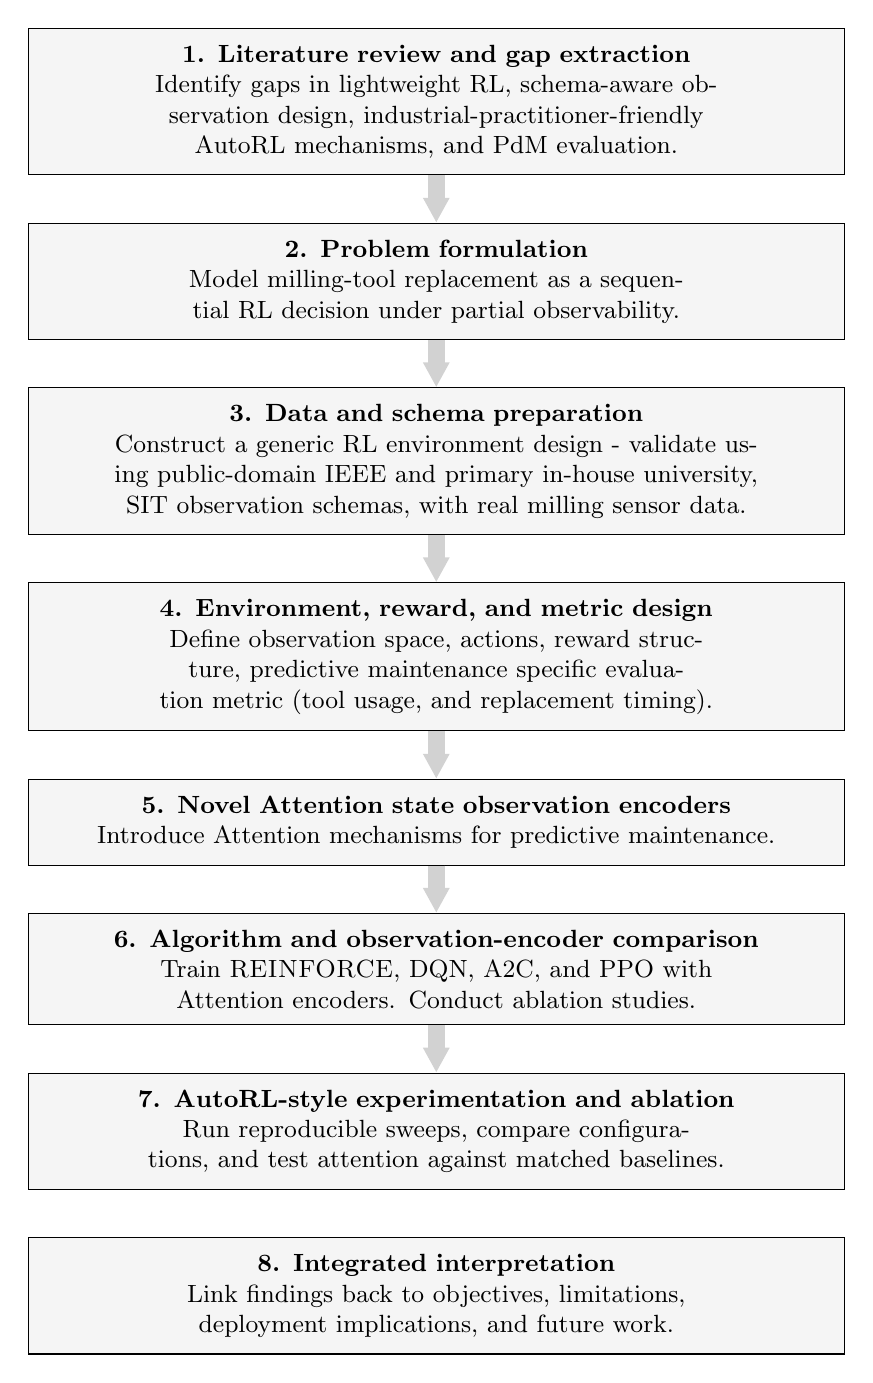
\begin{tikzpicture}[node distance=8mm, every node/.style={font=\small}]
		\tikzset{
			methodbox/.style={rectangle, draw=black, fill=gray!8, align=center, text width=0.82\textwidth, inner sep=6pt},
			arrowstyle/.style={draw=gray!35, line width=6pt, -{Triangle[length=9pt,width=9pt]}, rounded corners=2pt}
		}

		\node[methodbox] (b1) {\textbf{1. Literature review and gap extraction}\\Identify gaps in lightweight RL, schema-aware observation design, industrial-practitioner-friendly AutoRL mechanisms, and PdM evaluation.};
		\node[methodbox, below=6mm of b1] (b2) {\textbf{2. Problem formulation}\\Model milling-tool replacement as a sequential RL decision under partial observability.};
		\node[methodbox, below=6mm of b2] (b3) {\textbf{3. Data and schema preparation}\\Construct a generic RL environment design - validate using public-domain IEEE and primary in-house university, SIT observation schemas, with real milling sensor data.};
		\node[methodbox, below=6mm of b3] (b4) {\textbf{4. Environment, reward, and metric design}\\Define observation space, actions, reward structure, predictive maintenance specific evaluation metric (tool usage, and replacement timing).};
		\node[methodbox, below=6mm of b4] (b5) {\textbf{5. Novel Attention state observation encoders}\\Introduce Attention mechanisms for predictive maintenance.};
		\node[methodbox, below=6mm of b5] (b6) {\textbf{6. Algorithm and observation-encoder comparison}\\Train \textsc{REINFORCE}, DQN, A2C, and PPO with Attention encoders. Conduct ablation studies.};
		\node[methodbox, below=6mm of b6] (b7) {\textbf{7. AutoRL-style experimentation and ablation}\\Run reproducible sweeps, compare configurations, and test attention against matched baselines.};
		\node[methodbox, below=6mm of b7] (b8) {\textbf{8. Integrated interpretation}\\Link findings back to objectives, limitations, deployment implications, and future work.};

		\draw[arrowstyle] (b1.south) -- (b2.north);
		\draw[arrowstyle] (b2.south) -- (b3.north);
		\draw[arrowstyle] (b3.south) -- (b4.north);
		\draw[arrowstyle] (b4.south) -- (b5.north);
		\draw[arrowstyle] (b5.south) -- (b6.north);
		\draw[arrowstyle] (b6.south) -- (b7.north);
	\end{tikzpicture}
	\caption{High level Methodology flow-chart.}
	\label{fig:intro-method-flow}
\end{figure}

The method then represents milling-tool replacement as an RL environment in which an agent observes machine-condition information, chooses an action, receives a reward, and transitions to the next decision point. Because the true wear state is not continuously visible during production, the formulation is treated as partially observable in practice while using an MDP-style environment interface. The reward and evaluation metrics emphasize useful tool-life consumption, timely replacement, and threshold-violation avoidance.

The empirical workflow uses two schemas: the public IEEE milling benchmark and the in-house SIT milling schema. The algorithm set includes \textsc{REINFORCE}, DQN, A2C, and PPO, while the observation encoders include Nadaraya--Watson attention, temporal attention, multi-head attention, self-attention, and a no-attention baseline. A structured AutoRL-style pipeline trains, stores, evaluates, and compares these combinations under common scoring logic. The final ablation then tests whether attention-equipped policies outperform matched no-attention baselines.

Figure~\ref{fig:intro-method-flow} summarizes the methodology. The flow preserves the thesis chain of reasoning: literature gaps lead to research questions, the methodology defines environment and evaluation choices, the implementation realizes them in a reproducible pipeline, and the results test whether the resulting policies are useful under schema-aware evaluation.

\section{Organization of Thesis}

The thesis organization is as follows:

\begin{itemize}
	\item \textbf{Chapter~\ref{ch:literature-survey}: Literature Survey and Findings.} A systematic review of RL for predictive maintenance, covering problem formulations, algorithms, industrial applications, and research gaps that motivate the present work.
	\item \textbf{Chapter~\ref{ch:problem-statement}: Research Problem Statement and Objectives.} A synthesis of research gaps and a clear statement of the problem, research questions, and thesis objectives.
	\item \textbf{Chapter~\ref{ch:methodology}: Methodology.} The technical framework including the MDP formulation for milling-tool replacement, environment design, datasets, and evaluation metrics.
	\item \textbf{Chapter~\ref{ch:implementation}: Implementation Details.} Concrete implementation of the RL environment, algorithms (including REINFORCE), attention mechanisms, and the AutoRL experimental pipeline.
	\item \textbf{Chapter~\ref{ch:results}: Results and Discussion.} Experimental evidence from preliminary studies, the final schema-adaptive evaluation, an ablation study contrasting attention against no-attention baselines, and an integrated discussion with objective linkage.
	\item \textbf{Chapter~\ref{ch:conclusion}: Conclusions and Future Scope.} A summary of contributions, limitations, and suggested next steps for deployment-aware PdM using RL.
\end{itemize}



% -------------------------------------------------------------------
% Chapter 2: Literature Survey and Findings (primarily based on \citep{Siraskar2023SLR})
% -------------------------------------------------------------------

\chapter{Literature Survey and Findings}\label{ch:literature-survey}

\section{Chapter scope}
This chapter surveys research on applying reinforcement learning (RL) to predictive maintenance (PdM). The goal is to show how researchers formulate PdM as a sequential decision problem, which RL algorithms and environment models are used, which industrial settings are addressed, and which open challenges and opportunities remain.

Chapter~\ref{ch:introduction} introduced the thesis motivation together with essential background on milling, PdM, RL, and attention. Building on that foundation, this chapter presents the systematic literature review (SLR) process and extracts the survey findings that motivate the later methodology and experiments. The synthesis is presented through several structured tables so that readers can quickly understand the landscape.

Because the RL-for-PdM literature has grown rapidly, this chapter summarizes the body of work considered for the thesis as of May~2026. To keep the contribution logic clear, the synthesis also distinguishes prior art from the present author's publications: the external literature is first summarized after excluding the present author's papers, and the link from identified gaps to the thesis contributions is then stated explicitly.

\section{Positioning of the survey in existing reviews}
The application of RL to PdM has only recently started to attract dedicated survey attention. Prior review papers often treat RL as one technique among several machine-learning methods, or focus on adjacent themes such as anomaly detection or digital twins. Table~\ref{tbl:slr-survey-articles} contrasts representative review articles.

\newgeometry{margin=0.5in}
\begin{landscape}
\begin{table}[p]
	\renewcommand{\arraystretch}{1.3}
	\begin{minipage}{\textwidth}
		\caption{Positioning of the survey in existing reviews}\label{tbl:slr-survey-articles}
		\begin{tabular}{@{}L{4cm} L{1.5cm} L{1.75cm} C{1.2cm} L{2cm} L{1.5cm} L{1cm} L{1.2cm} L{7.5cm} @{} }
			\toprule
			Survey paper &PdM focused?&RL focused?\footnotemark[1]&Articles&Performance evals.?&RL taxonomy?&Case- studies?& Math treatment? & Focus / Other notes\\
			\midrule
			\cite{Net26} & PdM & RL only & 160 & {\sffamily x}&$\checkmark$& {\sffamily x}& {\sffamily x}&Lacks deep analysis, no case-studies. Basic taxonomy.\\
			\cite{Bor26} & PdM&RL only & 11 &{\sffamily x}&{\sffamily x}&{\sffamily x}&{\sffamily x}&Only offshore wind-farm maintenance\\
			\cite{Panzer2021}&All ops.&RL only&8&$\checkmark$&{\sffamily x}&{\sffamily x}&{\sffamily x}&Production systems\\
			\cite{Erhan2021}&All ops.&ML+RL&5&{\sffamily x}&$\checkmark$&{\sffamily x}&{\sffamily x}&Anomaly detection only. High-level taxonomy.\\
			\cite{Barja-Martinez2021}&All ops.&ML+RL&1&{\sffamily x}&{\sffamily x}&{\sffamily x}&{\sffamily x}&Big-data services for power distribution.\\			
			\cite{Ren2021}&PdM&ML+RL&5&{\sffamily x}&{\sffamily x}&{\sffamily x}&$\checkmark$&Light mathematical treatment\\
			\cite{Khan202013}&PdM&ML+RL&2&{\sffamily x}&{\sffamily x}&{\sffamily x}&{\sffamily x}&Focused on digital twin technologies.\\
			\cite{Mattioli2020}&PdM&ML+RL&1&{\sffamily x}&{\sffamily x}&{\sffamily x}&{\sffamily x}&Symbolic AI combined with ML\\
			\cite{Fink2020}&PdM&ML+RL&2&{\sffamily x}&{\sffamily x}&{\sffamily x}&{\sffamily x}&Industrial PHM\\
			\cite{Zonta2020}&PdM&ML only&0&{\sffamily x}&$\checkmark$&{\sffamily x}&{\sffamily x}&Exhaustive taxonomy. Limited to ML methods only.\\
			\midrule
			Present survey&\textbf{PdM}&\textbf{RL only}&\textbf{108}&\quad\textbf{$\checkmark$}&\textbf{$\checkmark$}&\textbf{$\checkmark$}&\textbf{$\checkmark$}&Focussed with extensive literature coverage.\\
		\end{tabular}
		\footnotetext[1]{``ML'' includes conventional ML and deep learning and ``RL'' includes deep RL.}
	\end{minipage}
\end{table}
\end{landscape}
\restoregeometry

\section{Systematic literature review methodology}
We follow a structured, multi-stage process to identify, screen, and analyze research publications \citep{Templier2015}. The search strategy was designed to capture RL work across three prognostics perspectives: early anomaly detection, early fault prediction, and remaining useful life (RUL) prediction, as well as maintenance-planning and scheduling formulations.

\subsection{Research questions}
The survey questions are listed in Table~\ref{tbl:slr-rq}. These questions guide the taxonomy, problem formulations, and synthesis presented later in this chapter.

\begin{table}[h]
	\renewcommand\arraystretch{1.5}
	\begin{center}
		\begin{minipage}{\textwidth}
			\caption{Research objectives of the SLR}\label{tbl:slr-rq}
			\begin{tabular}{@{}L{2cm} L{14cm} @{}}
				\toprule
				RQ & Research question\\
				\midrule
				RQ-1 & What taxonomies for RL methods exist for the PdM domain?\\
				RQ-2 & How are PdM problems formulated as RL tasks (state, action, reward, and environment)?\\
				RQ-3 & What industrial applications have been studied for RL-based PdM?\\
				RQ-4 & Which RL algorithms have been used and compared successfully?\\
				RQ-5 & Which datasets and evaluation metrics are used in the literature?\\
				RQ-6 & What challenges are reported when applying RL to PdM?\\
				RQ-7 & What future directions are suggested by researchers?\\
				\bottomrule
			\end{tabular}
		\end{minipage}
	\end{center}
\end{table}

\subsection{Search and screening process}
Figure~\ref{fig:slr-method} summarizes the survey pipeline in \cite{Siraskar2023SLR}, including screening and quality assessment.

\begin{figure}[!h]
	\centering
	\includegraphics[width=\columnwidth]{Fig3.pdf}
	\caption{Systematic literature research based on the \cite{Templier2015} process. Numbers indicate articles arrived after previous step process.}
	\label{fig:slr-method}
\end{figure}

The initial search covered Scopus\textsuperscript{\texttrademark}, Web of Science\textsuperscript{\texttrademark}, and IEEE Xplore\textsuperscript{\texttrademark}. Table~\ref{tbl:slr-mining} summarizes the article mining outcomes.

\begin{table}[h]
	\begin{center}
		\begin{minipage}{\textwidth}
			\caption{Article mining outcomes across databases}\label{tbl:slr-mining}
			\begin{tabular}{@{}L{2.5cm}R{1.5cm}R{1.5cm}R{1.5cm}R{1.5cm}R{1.5cm}R{1.5cm}R{1.5cm}@{}}
				\toprule
				& Base- line articles & Books, Reviews, Others & Intra- source duplicates & Inter- source duplicates& Title filter& Abstract \& Content filter & Final selection\\
				\midrule				
				Condition Based Maintenance      & 47 & 2  & 1 & 16 & 4 & 10 & \textbf{14}\\
				Anomaly Detection                & 32 & 11 &   & 9  & 8 & 1  & \textbf{3}\\
				Fault Diagnostics                &120 & 24 & 12& 33 &16 & 20 & \textbf{15}\\
				Remaining Useful Life Prediction & 15 & 1  & 8 & 3  &   &    & \textbf{3}\\
				Preventive Maintenance           & 83 &    & 40& 1  & 5 & 1  & \textbf{36}\\
				Predictive Maintenance           & 64 & 12 & 11& 23 & 2 & 2  & \textbf{14}\\
				Prescriptive Maintenance         & 5  &    & 2 & 3  &   &    & \\
				Prognostic Health Management     & 34 & 2  & 11& 5  & 2 & 1  & \textbf{13}\\
				All inclusive query              & 64 & 4  &   & 59 &   &    & \textbf{1}\\
				\midrule
				\textbf{Total} & \textbf{464} & \textbf{56} & \textbf{85} & \textbf{152} & \textbf{37} & \textbf{35} & \textbf{99}\\
				\multicolumn{7}{r}{Individually discovered articles: } & 9\\
				\midrule
				\multicolumn{7}{r}{\textbf{Grand Total:}} & \textbf{108}\\
				\bottomrule
			\end{tabular}
		\end{minipage}
	\end{center}
\end{table}

\section{Quantitative analysis of the literature}\label{sec:slr-quantitative}
The quantitative summary in \citep{Siraskar2023SLR} provided an early snapshot of the RL-for-PdM literature and the methodological base for the analysis here. The following figures and tables summarize the literature considered for this thesis, including studies available up to May~2026.

Figure~\ref{fig:slr-byyear} shows the year-wise distribution of research articles. The distribution indicates that RL-for-PdM is a recent, fast-growing area, with most papers concentrated in the 2020--2026 period. This concentration in the most recent years (Figure~\ref{fig:slr-byyear}), indicates that many design choices are still in flux and have not yet converged to standard baselines.

The Scopus-based quantitative analysis is summarized by publication year and contributing author in Figure~\ref{fig:slr-scopus}. The author-level view includes two publications by the present author.

\begin{figure}[!h]
	\centering
	\begin{subfigure}[b]{0.475\textwidth}
		\centering
		\includegraphics[width=\textwidth]{ArticlesByYear.png}
		\caption{Articles by year}
		\label{fig:slr-byyear}
	\end{subfigure}
	\hfill
	\begin{subfigure}[b]{0.475\textwidth}
		\centering
		\includegraphics[width=\textwidth]{Authors.png}
		\caption{Contributing authors}
		\label{fig:slr-byauthor}
	\end{subfigure}
	\caption{Scopus\textsuperscript{\texttrademark} analysis (May-2026)}
	\label{fig:slr-scopus}
\end{figure}

\subsection{Structure of the application literature}
Across primary studies, the application literature supports a two-stream structure. One stream treats maintenance as degradation-aware control, often with health states observed directly or engineered into the state representation \citep{Zha20,You20,You21,Hua20,Che22}. The second stream is closer to modern predictive-maintenance pipelines and uses sensor-derived health information or remaining useful life (RUL) estimates as inputs to the decision policy \citep{Bel19,Sko20,Lee22,Zha23,Xu25}. The first stream is larger and more mature; the second stream is smaller but more distinctly PdM-oriented and therefore central for a thesis framed around predictive maintenance rather than generic maintenance optimization.

Within this structure, the strongest anchors in the application literature include multi-component condition-based maintenance \citep{Zha20}, production-coupled maintenance \citep{Hua20}, probabilistic RUL integrated with deep RL \citep{Lee22}, sensor-driven real-time maintenance decision making \citep{Sko20}, and PHM feedback-loop formulations linking prognostics to decisions \citep{Bel19}.

\subsection{Using \texorpdfstring{$tf$--$idf$}{tf-idf} to identify novel concepts}

Most bibliographic analyses rely on standard key-term tools that highlight frequently occurring terms such as ``reinforcement learning'', ``predictive analytics'', and ``decision making''. Such frequency counts do not reveal distinctive approaches, application areas, or other differentiating features of the literature. To address this limitation, this thesis applies the natural-language-processing technique Term Frequency--Inverse Document Frequency ($tf$--$idf$) to analyze key terms.

$tf$--$idf$ vectorizes text by converting terms into numerical scores that indicate their relative importance within a document and across the document collection.

This method was applied to the titles, abstracts, and keywords of the articles. It assigns lower scores to the most frequently occurring terms and allows more distinctive terms to surface. Scores ranged from 1.4054 to 6.4548, with the lowest score assigned to ``reinforcement learning'', the term that appeared in every document. The most informative terms typically lie in the higher one-third to two-thirds range of scores. Figure~\ref{fig:slr-tfidf} highlights techniques surfaced by this method, including Petri nets for discrete-event system modeling, particle filters, the Chapman--Kolmogorov equation, multi-agent methods, and ant- and swarm-optimization techniques.

\begin{figure}[!h]
	\centering
	\includegraphics[trim={1cm 13cm 0cm 2cm}, clip, width=0.78\textwidth]{Fig6.pdf}
	\caption{Inverse $tf$--$idf$ driven identification of salient topics, adapted from \citep{Siraskar2023SLR}}
	\label{fig:slr-tfidf}
\end{figure}

\subsection{Highlighted research gaps}
The application literature is not evenly developed across five focus areas relevant to this thesis. Table~\ref{tbl:slr-focus-maturity} summarizes the maturity reading and its interpretation for the systematic survey.

This asymmetry is analytically important for the thesis. It shows that while RL-for-PdM is now a substantial application area, the literature remains uneven across (i) algorithmic families (notably REINFORCE), (ii) deployment constraints (edge-friendly design), and (iii) systematic, reproducible model-selection workflows (AutoRL-style experimentation). The thesis therefore treats observation design and algorithm selection as joint design choices rather than assuming that larger models or more complex optimizers will be superior out of the box.

\begin{table}[htbp]
	\renewcommand{\arraystretch}{1.3}
	\centering
	\begin{minipage}{\textwidth}
		\caption{Maturity of five focus areas in the application literature}\label{tbl:slr-focus-maturity}
		\begin{tabular}{@{}L{0.30\linewidth}L{0.36\linewidth}L{0.30\linewidth}@{}}
			\toprule
			\textbf{Focus area} & \textbf{Reading of the literature} & \textbf{Analysis}\\
			\midrule
			RL for PdM overall & Established and growing application core & Strong enough for a structured SLR narrative\\
			Attention mechanisms for PdM & Emerging but still thin \citep{Zha23,Guo26,Li25} & Frontier topic rather than a mature cluster\\
			AutoRL for PdM & No clear papers in the surveyed literature & White-space topic\\
			REINFORCE for PdM & No clear papers in the surveyed literature & Clear methodological gap\\
			Edge and Industry~4.0 RL for PdM & Distinct deployment-oriented substream \citep{Ong20,Ong22,Ong22b,Tha23,Yan23} & Strongest specialized stream after the main literature core\\
			\bottomrule
		\end{tabular}
	\end{minipage}
\end{table}

\section{Evolution of predictive maintenance methods}\label{sec:evolution}
Before narrowing the discussion to RL, the survey first positions PdM within the broader evolution of maintenance research. Predictive maintenance has advanced from ad-hoc and rule-based practices to analytical reliability models, optimization-driven scheduling, and, more recently, data-driven machine learning and deep learning methods. The two-part taxonomy in Figures~\ref{fig:PdMEvolutionTaxonomy-1} and~\ref{fig:PdMEvolutionTaxonomy-2} separates the traditional, model-based lineage from the data-centric branch that encompasses ML and RL approaches. This ordering keeps the historical development of PdM distinct from the RL-specific taxonomy introduced in the next section.

\newgeometry{margin=0.5in}
\begin{landscape}
	\begin{figure}[!h]
		\centering
		\includegraphics[width=\linewidth]{Fig9.pdf}
		\caption{
			Taxonomy Part I: Traditional methods for PdM}
		\label{fig:PdMEvolutionTaxonomy-1}
	\end{figure}
\end{landscape}

\begin{landscape}
	\begin{figure}[!h]
		\centering
		\includegraphics[width=\linewidth]{Fig10.pdf}
		\caption{Taxonomy Part II: Data-based methods for PdM (ML and RL)}
		\label{fig:PdMEvolutionTaxonomy-2}
	\end{figure}
\end{landscape}
\restoregeometry

\subsection{Origins: statistical reliability methods}
The earliest scientific PdM methods used parametric lifetime models to describe time-to-failure. A continuous lifetime variable is fitted to a chosen probability distribution (for example exponential, normal, log-normal, or Weibull) and used to estimate failure probabilities and schedule preventive actions \citep{mann1995,weibull1951,Abernethy}.

For the Weibull model the reliability (survival) function is commonly written as
\begin{equation}\label{eq:Weibull}
	R(t) = e^{-\left(\dfrac{t}{\beta}\right)^{\alpha}},
\end{equation}
where $\alpha$ and $\beta$ are the shape and scale parameters. When $\alpha>1$ the failure rate is increasing and the model can be used directly to pick replacement intervals; when $\alpha\leq1$ different maintenance trade-offs arise \citep{mann1995}. Practitioners have extended these basic models (for example three-parameter Weibull fits) to estimate subsystem-level preventive intervals in heavy equipment domains \citep{Bala2018reliability}.

Stochastic distributions also appear inside RL-style PdM models: for example, gamma or Poisson laws are used to model time-between-failures, repair durations, or production demand while simpler uniform or exponential assumptions may describe repair or PM durations \citep{R-SMART-Gosavi2004}.

\subsection{KPI-based cost objectives}
Business KPIs were incorporated next, turning lifetime estimates into cost-aware decision rules. A standard objective is the long-run maintenance cost per unit time, which balances planned preventive maintenance cost $C_{PM}$ against corrective (unplanned) failure cost $C_{CM}$. For a component with reliability $R(t)$ an average cost rate can be written as
\begin{equation}\label{eq:TC}
	TC(t) = \dfrac{C_{PM}\,R(t) + C_{CM}\,(1-R(t))}{\int_{0}^{t} R(x)\,dx},
\end{equation}
and the optimal replacement interval minimizes $TC(t)$ \citep{mann1995}.

\subsection{Optimization and scheduling methods}
As systems grew in scale and complexity, scheduling and optimization techniques were introduced. Linear, nonlinear and mixed-integer programming formulations enabled joint optimization of maintenance and production schedules under constraints and multiple objectives \citep{russenschuck1999,LiZhaojun2016}. These methods perform well when the system dynamics and objectives can be expressed compactly, but they become brittle under nonlinear uncertainty or partial observability.

\subsection{Machine learning and deep learning}
Machine learning broadened PdM by learning mappings from sensor and operational data to diagnostics and prognostics. Techniques range from feature-based models (decision trees, random forests, gradient boosting, SVMs, PCA) to sequence models such as LSTMs for RUL estimation \citep{eke2017,scheibelhofer2012methodology,Kabir2018,Ren2021,Mattioli2020,Fink2020}.

Some deep-learning studies adopt engineered ``state-goals'' or normalized state representations rather than raw signals. For example, a voltage-based state-goal used in the literature normalizes deviations relative to a historical window via
\begin{equation}\label{eq:voltagestate}
	V_g = \begin{cases}
		1 - \dfrac{|V-\bar{V}|}{V_{max}-V_{min}}, & \text{if } V_{max}\neq V_{min},\\
		0, & \text{otherwise},
	\end{cases}
\end{equation}
which highlights sensitivity to the choice of look-back window and avoids feeding unbounded raw values into sequence models \citep{skydt2021}.

While ML and DL improved early fault detection and RUL prediction, these approaches typically rely on labelled failures and do not by themselves solve the sequential decision problem of when to act; this gap motivates the use of RL for PdM.

\section{Taxonomy of RL for predictive maintenance}
RL methods for PdM are grouped along two complementary dimensions: environment formulation and algorithm family. On the modeling side, fully observed MDPs remain the dominant choice, while POMDPs, hidden-state variants, and semi-Markov models appear when authors explicitly account for incomplete sensing, latent degradation, or irregular decision intervals. On the algorithm side, value-based methods remain the most common, with actor--critic and policy-search approaches becoming more visible in later work.

These distinctions matter here not as elementary background, but as evidence of how the field balances realism, tractability, and deployment constraints. They also position the present thesis within the surveyed design space before the chapter turns to specific PdM RL methods and case studies.

\begin{figure}[!h]
	\centering
	\includegraphics[width=\columnwidth]{Fig14.pdf}
	\caption{A taxonomy of RL for predictive maintenance \citep{Siraskar2023SLR}}
	\label{fig:RLPdMTaxonomy}
\end{figure}

\begin{figure}[!h]
	\centering
	\includegraphics[width=\columnwidth]{Fig15.pdf}
	\caption{A complexity and versatility view of RL algorithms}
	\label{fig:RLAlgoComparison}
\end{figure}

Figures~\ref{fig:RLPdMTaxonomy} and~\ref{fig:RLAlgoComparison} are therefore used as the organizing bridge between the general PdM evolution discussed above and the RL-specific formulations reviewed below. The next section narrows from taxonomy to concrete PdM formulations: state representation, reward design, semi-Markov timing, and representative case-study patterns.

\section{Reinforcement learning for predictive maintenance - A detailed analysis of algorithms and variants}

\subsection{Environment models and observability}
Many PdM problems are only partially observable in practice due to sensor noise, hidden degradation mechanisms, and changing operating conditions. Section~\ref{sec:intro-rl} in Chapter~\ref{ch:introduction} provides a comprehensive treatment of common Markov decision process (MDP) variants, including partially observable formulations (POMDPs), hidden-mode MDPs, semi-Markov decision processes (SMDPs), and semi-POMDPs. These formulations preserve the sequential-decision structure while accommodating indirect sensing and variable decision timing. Figure~\ref{fig:MDPSMDP} illustrates these core technical distinctions.

PdM can be expressed as an RL problem by defining the observable health state, the possible maintenance actions, and a reward that reflects production loss, maintenance cost, and risk of failure. In a simple state diagram, the equipment degrades over time if no action is taken. Maintenance may return it to a healthier state, while replacement may restore it to an initial condition. If deterioration continues unchecked, the process reaches a terminal failure state.

\begin{figure}[!h]
	\centering
	\includegraphics[width=0.75\columnwidth]{Fig16.pdf}
	\caption{State diagram with possible PdM states}
	\label{fig:RLPdMStateDiagram}
\end{figure}

The reward function can combine operational profit, maintenance cost, repair cost, and penalties for downtime. This makes PdM a sequential decision problem rather than a pure prediction task.

\begin{figure}[!h]
	\centering
	\includegraphics[width=0.75\columnwidth]{Fig17.pdf}
	\caption{The PdM problem formulated as an RL problem}
	\label{fig:RLPdMFormulation}
\end{figure}

\subsection{The SMART family}\label{sec:smart-family}
One of the earliest algorithms developed explicitly for PdM-style industrial problems is SMART \citep{MahadevanSMART}. It is a model-free, average-reward method formulated for semi-MDPs. This makes it particularly effective for factory optimization where decisions are discrete events, but the time between them (the sojourn time) varies continuously. Furthermore, SMART uses a unique reward formulation: an immediate scalar reward is supplemented by an accumulated reward generated at a fixed rate until the next decision event.

The core learning update in SMART modifies the standard temporal difference method to optimize the average sum of rewards. Let the estimated value of taking action $a$ in state $s$ at decision epoch $n$ be $Q_n(s,a)$. The value is updated recursively via a stochastic approximation learning rate $\alpha_n$ according to:
\begin{equation}\label{eq:SMART}
	Q_{n+1}(s,a) \xleftarrow{\alpha_n} \left( r_{imm} - \rho_n \tau + \max_{a'} Q_n(s',a') \right)
\end{equation}
where $r_{imm}$ is the accumulated reward between epochs $n$ and $n+1$, $\tau$ is the transition time (sojourn time), $s'$ and $a'$ represent the state and action at the next epoch, and $\rho_n$ is the average reward rate. The reward rate effectively balances revenue ($R$) against corrective ($C_{\scriptscriptstyle{CM}}$) and preventive ($C_{\scriptscriptstyle{PM}}$) maintenance costs over the total elapsed time ($T$):
\begin{equation}\label{eq:rho}
    \rho = \frac {R - C_{\scriptscriptstyle{CM}} - C_{\scriptscriptstyle{PM}}} {T}
\end{equation}

By accommodating large state spaces and incorporating non-uniform time transitions, SMART demonstrated superior average rewards compared to existing heuristic operating policies. Alongside the related Q-P learning algorithm \citep{gosavi2004qp}, SMART prompted several improved variants over time. Table~\ref{tbl:SMART_evolution} outlines how the algorithm evolved to address exploration limitations and convergence stability.
	
\begin{table}[h]
	\renewcommand{\arraystretch}{1.5}
	\begin{center}	
		\begin{minipage}{\textwidth}
			\caption{Evolution of the SMART algorithm family}\label{tbl:SMART_evolution}
			\begin{tabular}{@{}L{1.5cm} L{3.5cm} L{10cm}@{}}
				\toprule
				\textbf{Year} & \textbf{Algorithm} & \textbf{Key contributions and notes}\\
				\midrule
				1997 & SMART \par \citep{MahadevanSMART} & Introduced the semi-MDP average-reward modeling for continuous-time industrial processes. Showed higher average-reward than robust heuristic replacement models.\\
				1999 & SMART \par \citep{SMART-Das1999} & Provided formal convergence proofs for the SMART algorithm operating over an infinitely long time horizon.\\
				2004 & R-SMART \par \citep{R-SMART-Gosavi2004} & Introduced a relaxation scheme for updating the average reward $\rho$. Performance was heavily dependent on manually tuning an exploration decay rate to ensure convergence.\\
				2017 & iSMART \par \citep{iSMART-Encapera2017} & Overcame R-SMART's decay limitations by utilizing a constant exploration rate, proving more robust while demonstrating a roughly 30\% increase in average reward.\\
				\bottomrule
			\end{tabular}
		\end{minipage}
	\end{center}
\end{table}

\subsection{Algorithms and datasets used for evaluation}
Across the literature, Q-learning and its deep variants are the most frequently used methods. Actor--critic and policy-gradient methods follow, with PPO and DDPG appearing in more recent work. MDPs remain the most common environment model, followed by SMDPs. Figure~\ref{fig:slr-algo-chart} summarizes these environment-modeling and algorithm trends, while Table~\ref{tbl:AlgorithmSelection} translates the same evidence into a compact selection view for PdM researchers.

\begin{figure}[!h]
	\centering
	\includegraphics[width=0.6\textwidth]{Fig18.pdf}
	\caption{Prominent environment modeling techniques and RL algorithms}
	\label{fig:slr-algo-chart}
\end{figure}

\begin{table}[htbp]
	\begin{center}
		\begin{minipage}{\textwidth}
			\caption{Selecting an RL algorithm in PdM - Considerations to be made}\label{tbl:AlgorithmSelection}
			\renewcommand{\arraystretch}{1.4}
			\begin{tabular}{L{3.0cm} L{4cm} L{4cm} L{4cm}}
				\toprule
				 & \textbf{Q-learning family} & \textbf{Policy Gradient methods} & \textbf{Actor Critic methods}\\
				\midrule
				\textbf{Observation space} & Discrete or continuous & Discrete or continuous & Discrete or continuous\\
				\textbf{Action space} & Discrete & Discrete or continuous & Discrete or continuous\\
				\textbf{Advantages} & Simple and stable baseline in many discrete-action settings & Direct policy optimization and continuous actions & Better sample efficiency with value estimation\\
				\textbf{Disadvantages} & Needs function approximation in large spaces & Can be sample-inefficient and sensitive to reward scaling & Higher compute and tuning complexity due to dual networks\\
				\bottomrule
			\end{tabular}
		\end{minipage}
	\end{center}
\end{table}

\newgeometry{margin=0.5in}
\begin{landscape}
	\begin{table*}[h]
		\renewcommand{\arraystretch}{1.3}
		\begin{minipage}{\textwidth}
			\caption{Scenarios of PdM along with challenges addressed by researchers}\label{tbl:AgoDetails}
			\begin{tabular}{@{}L{3.5cm}L{5.5cm}L{5.5cm}L{8cm}@{}}
				\toprule
				\textbf{Article} & \textbf{Scenario} & \textbf{Challenges addressed} & \textbf{RL methods applied}\\
				\midrule
				\cite{Cheng2018} & Bearing degradation and change-point detection & Simultaneous HI and change-point detection & Q-learning with engineered health indicators.\\
				\cite{Li2020GA} & Manufacturing (large-scale) with buffers & State/action explosion and noisy rewards & Multi-agent RL combined with a genetic algorithm.\\
				\cite{Wang20149} & Machine (singular) with multiple yield levels & Imperfect maintenance and hidden yield states & Q-P algorithm and hidden semi-Markov modeling.\\
				\cite{Andriotis2021} & Multi-component deteriorating system & Incomplete information, dimensionality, stochasticity, and measurement variability & Deep decentralized multi-agent actor critic with constrained POMDP formulation.\\
				\cite{Afshari2014} & RUL estimation for roller bearings & Non-stationary stochastic estimation & Auto-step RL with Paris-law crack propagation model.\\
				\cite{Skordilis2020} & Turbofan RUL and maintenance policy generation & Real-time control, uncertainty, and partial observability & Deep RL with particle filtering and hybrid state-space modeling.\\
				\cite{Yan201992110} & Lubricating oil replacement in oil-field machinery & Multi-source spectral analysis and health index construction & Wiener-process degradation model, entropy-based health index, and value iteration.\\
				\cite{Ling2018364} & Dual-machine flow line with buffer and limited maintenance resources & Independent deterioration and imperfect PM & Distributed SMART, a multi-agent average-reward SMDP approach.\\
				\cite{Feng202218910} & Multistage production systems with bottlenecks & Bottleneck identification without closed-form expressions & Q-learning and approximate dynamic programming for joint production and maintenance.\\
				\bottomrule
			\end{tabular}
		\end{minipage}
	\end{table*}
\end{landscape}
\restoregeometry

The datasets used for evaluation vary widely, but NASA turbofan degradation data appears most frequently. CWRU bearing data, PRONOSTIA bearing data, and simulation-based industrial line data are also common. Evaluation metrics are less consistent than in standard classification work. Average reward is common, but industrial metrics such as OEE, downtime reduction, and maintenance cost are also used.

%% Algorithms applied by researchers (standard and their variants)
\begin{table}[h]
	\renewcommand\arraystretch{1.5}
	\begin{center}
		\begin{minipage}{\textwidth}
		\caption{Algorithms researched (Both baseline algo. and variants)}\label{tbl:AlgoListStandard}
		\begin{tabular}{@{} R{0.5cm} L{4cm} L{8cm} @{}}
		\toprule
		&\textbf{Algorithms}&\textbf{Articles}\\
		\midrule
		1&Q-Learning and Deep Q-network (DQN)&\cite{Skordilis2020, Wang2021Integrated, Zhang2022156, Adams2019, Cheng2021, Correa-Jullian2020, Epureanu2020, dong2021WT, HoongOng2020, Hu2021, Huang2019523, Huang2020, Martinez20182030, Rocchetta2019291, Senthil2022, Jha2019171, Jha2019418, Tanimoto202146788, Dai20208307, Ding2019, Zhang2021, Zhang2020}\\
		2&Actor-Critic algorithms& \cite{Liu2017299, Liu2020166, Andriotis2019, Hosseinloo2021, Wang2021FaultDiagnosis, Shuvo2020, Su2022}\\
		3&PPO&\cite{Pinciroli2021, Pinciroli2022752, Kuhnle2019, Ong2021}\\
		4&DDPG&\cite{Hosseinloo2021, Chen2022484}\\
		&\multicolumn{2}{l}{\textbf{Complex objectives and ensemble methods:}}\\
		5&Multi-agent formulation&\cite{Kuhnle2019, Su2022, Andriotis2019, Andriotis2021, Wang2016325}\\
		6&Multi-objective formulation& \cite{Lepenioti20205}\\	
		\bottomrule
		\end{tabular}
		\end{minipage}
	\end{center}
\end{table}


%% Specialized and novel algorithms applied by researchers
\begin{table}[h]
	\renewcommand\arraystretch{1.5}
	\begin{center}
		\begin{minipage}{\textwidth}
			\caption{Novel and special RL for PdM algorithms}\label{tbl:AlgoListSpecialized}
			\begin{tabular}{@{} R{0.5cm} L{6.5cm} L{6.5cm}@{}}
				\toprule
				&\textbf{Algorithms}&\textbf{Articles}\\
				\midrule
				1&Q-P learning algorithm -- Original design:& \cite{gosavi2004qp}\\
				2&Q-P learning algorithm -- Application:& \cite{ Min2012176, Wang20149}\\
				3&HITDFA -- Health Indicator Temporal-Difference Learning with Function Approximation&\cite{Zhang2019488}\\
				4&Health Stage Change Points detection using RL&\cite{Cheng2018}\\
				5&Particle filtering using RL& \cite{Skordilis2020}\\
				6&Neural architecture parameter search (NAS), using RL & \cite{Eltotongy2021117}\\
				7&Continuous wavelet transforms (CWT), using RL& \cite{Eltotongy2021117}\\
				8&Reinforcement Lion Swarm Optimization Algorithm & \cite{Dai2021}\\
				9&Petri Nets and RL & \cite{Mao2021}\\
				10&Markov Mixed Membership Models (MMMM) and POMDP & \cite{Hofmann2020464}\\
				\bottomrule
			\end{tabular}
		\end{minipage}
	\end{center}
\end{table}
	
%% MDP model formulation
\begin{table}[h]
\renewcommand\arraystretch{1.5}
\begin{center}
	\begin{minipage}{\textwidth}
		\caption{MDP model formulation}\label{tbl:XMarkovFormulation}
		\begin{tabular}{@{} R{0.5cm} L{6.5cm} L{6.5cm}@{}}
			\toprule
			&\textbf{Markov Model Formulation}&\textbf{Articles}\\
			\midrule
			1&MDP&\cite{R-SMART-Gosavi2004, Gosavi2016235, Mikhail2019133, Shi2019, Andriotis2019, Barde2019147, Chen2022484, Paraschos2020470, Yang2021, Yang201880}\\
			2&HM-MDP (Hidden Mode MDP)&\cite{Hofmann2020464, Yang20131647}\\
			3&SMDP (Semi MDP)&\cite{Ling2018364, Adsule2020182, R-SMART-Gosavi2004, SMART-Das1999, iSMART-Encapera2017, Wang20149, Hosseinloo2021, Wang2021PredictiveMaintenance, Wang2016325, Wang2015614}\\
			4&H-SMDP (Hidden Semi MDP)&\cite{Wang20149}\\
			5&POMDP (Partially Observable MDP)&\cite{Hofmann2020464, Andriotis2019, Andriotis2021}\\
			6&Markov Mixed Membership Models (MMMM) and POMDP & \cite{Hofmann2020464}\\
			\bottomrule
		\end{tabular}
	\end{minipage}
\end{center}
\end{table}
	
%% Begin Industrial application sections
\section{Industrial applications and use cases}
The literature covers a broad set of PdM use cases. Rotating machinery, bearings, gearboxes, milling equipment, hydraulic systems, and multi-machine production lines are all represented. In many studies, the RL model is used to identify a point of health change or to schedule the next maintenance action.

For rotating machines, the survey highlights RL used alongside signal processing and neural models to detect faults earlier. For production lines, the emphasis shifts to buffer levels, machine age, downtime costs, and coordination across machines. In these settings, maintenance and production are interdependent, so the action for one machine affects the state of the whole line.

\subsection{Maintenance of assembly lines and multi-machine systems}
The surveyed work includes a detailed comparison of studies on serial production lines and systems with intermediate buffers. The common pattern is to model the system as an MDP, define maintenance actions per machine, and use a reward that penalizes lost production and maintenance cost. Multi-agent and heuristic-assisted methods are useful when the state space becomes too large for a single controller.

\newgeometry{margin=0.5in}
\begin{landscape}
	\begin{table}[p]
		\renewcommand{\arraystretch}{1.3}
		\begin{minipage}{\textwidth}
			\caption{A comparison of implementations for maintenance of assembly lines and multi-machine systems}\label{tbl:SchedulePM}
			\begin{tabular}{@{}L{3.5cm}L{2.5cm}L{3.5cm}L{1.5cm}L{1.5cm}L{9.5cm}@{}}
				\toprule
				\textbf{Use-case} & \textbf{Article} & \textbf{Algorithm} & \textbf{Agent} & \textbf{MDP} & \textbf{Notes}\\
				\midrule
				Industrial edge IoT & \cite{Ong2021} & PPO with LSTM & Single-agent & MDP & Better performance than conventional RL and improved learning efficiency on NASA C-MAPSS.\\
				Pumping system RUL & \cite{Bellani2019PHM} & Q-learning & Single-agent & MDP & Better average reward than heuristic baselines in low- and high-performance settings.\\
				Serial production line & \cite{Huang2020} & Q-learning / DQN & Single-agent & MDP & State includes machine age, buffer levels, and remaining maintenance duration; simulation with six machine interleaved with buffers; lower maintenance cost than age-dependent PM and opportunistic maintenance.\\
				Serial production line & \cite{Huang2019523} & Q-learning / DQN & Single-agent & MDP & Models four degradation states and one failure state; 3-machine, 2-buffer simulation; about 70\% improvement over corrective maintenance.\\
				Bearings and change-of-health detection & \cite{Cheng2018} & Q-learning with Calinski-Harabasz reward & Single-agent & MDP & Correctly identifies health stages in the PRONOSTIA dataset.\\
				Aerospace maintenance & \cite{Hu2021} & Q-learning with extreme learning machine & Single-agent & MDP & Long-term maintenance. Higher reward than PM and corrective maintenance.\\
				DC motor shaft wear RUL & \cite{Jha2019171} & Q-learning & Single-agent & MDP & Learns an offline control policy with wear modeled by Archard's law.\\
				Component layer thickness wear & \cite{Adsule2020182} & SMART family algorithm & Single-agent & continuous-time SMDP & Learns an optimal policy in about 1000 steps on a 100-state problem.\\
				Large-scale manufacturing & \cite{Li2020GA} & Q-learning and GA-assisted MARL & Multi-agent & MDP & Applies intermediate buffers. Genetic algorithm improves convergence and average revenue over pure RL and pure GA.\\				
				\bottomrule
			\end{tabular}
		\end{minipage}
	\end{table}
\end{landscape}
\restoregeometry

%% Environments and data-set used for evaluation
\begin{table}[h]
\renewcommand\arraystretch{1.5}
\begin{center}
	\begin{minipage}{\textwidth}
		\caption{Environments and data-set used for evaluation}\label{tab:data-set}
		\begin{tabular}{@{} R{0.5cm} L{8cm} L{4cm}@{}}
			\toprule
			&\textbf{Evaluation data-set}&\textbf{Publications}\\
			\midrule
			1&Turbofan Engine Degradation Simulation Data Set, NASA \citep{NASATurbofan}.\par Engine run-to-failure time-series \textit{simulated} data (using C-MAPSS tool). Four different data-sets simulated under different combinations of operational conditions and fault modes. & \cite{Skordilis2020, Ong2021, HoongOng2020, Zhang2019488}\\
			2&CWRU (Case Western Reserve University) bearing failure data-set \citep{CWRUBearingDataset}.&\cite{Ding2019, Eltotongy2021117}\\
			3&PRONOSTIA bearing failure data-set \citep{Pronostia2012}.&\cite{Cheng2018}\\
			4&UCR Timeseries \citep{UCRArchive2018}. Three data sets are used for evaluation: (1) Gun-point (2) Wafer (3) ECG. Of these, only the ``wafer'' data-set is related to the PdM field and contains inline process control measurements, classified as normal and abnormal.&\cite{Martinez20182030}\\
			5&Milling cutter run-to-failure data for 3 cutters: force, vibration and acoustic emission. Wear measurement by LEICA MZ12 microscopy system \citep{PHM2010MillingCutterDataset};&\cite{Dai2021}\\
			6&\textit{Simulated} wind-farm of 50 wind-turbines using failure rate of wind-turbines from \citep{ozturk2018}.& \cite{Pinciroli2021}\\
			\bottomrule
		\end{tabular}
	\end{minipage}
\end{center}
\end{table}

%% Industrial applications (RQ-3)
\renewcommand*{\arraystretch}{1.2} {
\onehalfspacing
\begin{longtable}[H]{R{1cm} L{5cm} L{7cm}}
	\caption{Industrial applications (RQ-3)}\label{tbl:Industry}\\
	\toprule
	& Industry/Application & Articles\\
	\midrule
	\endfirsthead
	
	\multicolumn{3}{c}%
	{\tablename\ \thetable\ -- \textit{Continued from previous page}} \\
	\toprule
	& Industry/Application & Articles\\
	\midrule
	\endhead
	\midrule
	
	\endfoot		
	\bottomrule
	\endlastfoot
	1&Edge-based sensor networks&\cite{HoongOng2020}\\
	2&Milling machines (cutter tool wear)&\cite{Dai2021}\\
	3&Aerospace&\cite{Ahmed2018233, Dangut2022, Hu2021, Li20192133, Skordilis2020}\\
	4&Battery systems&\cite{Chen2011, Wu2021}\\
	5&Civil engineering (bridges, large systems)&\cite{Cheng2021, Andriotis2019, Shi2019, Yang2022}\\
	6&Chemical industry&\cite{Wang2021FaultDiagnosis}\\
	73&Lubrication oil&\cite{Yan201992110}\\
	8&Oil and gas&\cite{Compare202052}\\
	9&Petroleum industry&\cite{Aissani20091089, Min2012176}\\
	10&Coal industry&\cite{Liu2020166}\\
	11&Gas turbines (gas path faults)&\cite{Compare202052, Luo2021}\\
	12&Wind turbines and wind farms &\cite{Pinciroli2021, Pinciroli2022752, dong2021WT, Eltotongy2021117, Pinciroli20201476}\\
	13&Hydraulic actuators& \cite{Adams2019}\\
	14&Infrastructure maintenance (complex and large-scale) &  \cite{Tanimoto202146788}\\
	15&Iron and steel factories & \cite{Lepenioti20205}\\
	16&Military (trucks - fleet maintenance)&\cite{Barde2019147}\\
	17&Planning of maintenance inventory&\cite{SMART-Das1999, Xanthopoulos2017576}\\
	18&Power systems and grids (industrial)&\cite{Rocchetta2019291, Shuvo2020}\\
	19&Production and assembly lines (multiple machine and MIMO systems)&\cite{ Min2012176, Senthil2022, Ling2018364, Su2022, Cui20213416, Cui2022ADP, Huang2019523, Huang2020, Liu2017299, Paraschos2020470, Wang20149, Wang2016325, Wang2015614, Zhang2022156, Zhang2020, Zheng2017}\\
	20&Rotating machinery (bearing housings)&\cite{Ding2019, Afshari2014, Dai20208307, Skordilis2020, Dong2021343}\\
	21&Robotics&\cite{Li2021}\\
	22&Rubber industry (curing machines)&\cite{Senthil2022}\\
	23&Semiconductor manufacturing&\cite{valet2022opportunistic, Hoffmann2021simulative, scheibelhofer2012methodology}\\
	24&Solar systems&\cite{Correa-Jullian2020}\\
\end{longtable}
}	

\section{Simulation systems in practice}
As a practical bridge between field data and live deployment, the survey highlights several commercial and open-source simulation tools that support RL development before shifting policies to physical machinery. These tools vary in how natively they support RL, their ease of integration, and their best-suited industrial domains. Table~\ref{tbl:SimulationSystems} highlights key simulation platforms identified in the survey.

\begin{figure}[!h]
	\centering
	\includegraphics[width=\columnwidth]{Fig19.pdf}
	\caption{AnyLogic\textsuperscript{\texttrademark}: commercial simulation software (\href{https://www.anylogic.com/}{AnyLogic.com}) }
	\label{fig:AnyLogic}
\end{figure}

\begin{table*}[!htbp]
	\renewcommand\arraystretch{1.5}
	\begin{center}
		\begin{minipage}{\textwidth}
			\caption[Simulation systems]{Simulation systems\protect\footnote{\texttt{\$\$}: commercial; \texttt{OS}: open-source.}}\label{tbl:SimulationSystems}
			\begin{tabular}{@{}L{4.5cm} L{2cm} L{1.25cm} L{1.75cm} L{5cm}@{}}
				\toprule
				\textbf{Industry} & \textbf{Product \& Link} & \textbf{Type} & \textbf{RL support} & \textbf{Notes}\\
				\midrule				
				Production systems planning. Management of complex assembly lines & \href{https://github.com/AndreasKuhnle/SimRLFab}{SimRLFab} & \texttt{OS} & Integrated, easy & Native Python low-level development.\\
				Manufacturing, oil and gas, energy, mining, logistics & \href{https://www.anylogic.com/}{AnyLogic} & \texttt{\$\$} & Integrated, easy & Supports RESTful API integration with custom Python code and uncertainty modeling.\\
				Chemical process simulator & \href{https://dwsim.fossee.in/}{DWSim} & \texttt{OS} & Indirect, difficult & CAPE-OPEN compliant.\\
				Components such as pumps and wind turbines to buildings & \href{http://www.trnsys.com/}{TRNSYS} & \texttt{\$\$} & Indirect, difficult & Supports C and C++ integration.\\
				Robotics and physics-based simulations, safety simulation & \href{https://gazebosim.org/home}{Gazebo} & \texttt{OS} & Indirect, easy & Cloud-based services with a useful sensor library.\\
				\bottomrule
			\end{tabular}
		\end{minipage}
	\end{center}
\end{table*}

\section{Challenges and research gaps}\label{sec:slr-challenges}
We identify challenges that arise from both prognostics and RL.

\subsection{Inherent challenges of prognostics}
The ``paradox of prognostics'' highlights a practical limitation: validating a prediction often requires letting the asset fail, while acting on a prediction can prevent that failure and remove ground truth for evaluation \citep{Saxena2010evaluating}. In addition, prognostics is affected by acausality (future operating conditions influence the outcome) and by uncertainty in end-of-life estimation.

\subsection{Inherent challenges of deep RL}
Deep RL methods can be unstable and sensitive to reward design, scaling, and hyperparameter choices \citep{b_SONG,b_HENDERSON,b_HARDT,b_ZHANG,dulac2021}. Sparse rewards are common in PdM, and reward shaping can strongly influence learning behavior \citep{Grzes2017,Fink2020}. Deep RL methods are also known to exhibit issues such as overfitting to spurious correlations during exploration \citep{b_SONG} and variability due to stochasticity and random seeds \citep{b_HENDERSON}.

\subsection{State representation under uncertainty}
Real PdM deployments are affected by stochastic degradation, operational variability, and measurement noise. \cite{Andriotis2021} therefore emphasizes the need for richer and more realistic state representations, including partially observable formulations (POMDPs) for handling uncertainty. However, building realistic environments often requires degradation-to-failure data, which is expensive or impractical to collect.

\subsection{Evaluation inconsistency}
The survey identified a large variation in evaluation practices across studies, including the use of simulated versus public datasets, and inconsistent metrics. For prognostics-oriented applications, domain-specific metrics such as prognostic horizon and $\alpha$--$\lambda$ accuracy are recommended \citep{Saxena2010metrics,Saxena2010evaluating}.

\section{Opportunities and future research directions}\label{sec:slr-opportunities}
This section identifies which of these opportunities are directly or indirectly addressed in the present thesis research.

\subsection{Robust, risk-aware, and meta reinforcement learning}
Robust RL and risk-sensitive RL provide mechanisms to account for uncertainty and variability in transition dynamics, disturbances, actions, or observations \citep{moos2022robust}. Meta-RL can reuse experience gained in earlier tasks to adapt faster to new operating regimes; however, \citet{imagawa2022Meta} notes that these themes are under-explored in PdM.

\textit{Connection to this thesis:} This thesis evaluates the same MDP formulation across two different milling sensor schemas (IEEE and SIT), showing why policies must be selected jointly with the observation schema rather than treated as fixed across environments. This schema-awareness reflects an implicit robustness consideration, although explicit risk-sensitive RL is outside the thesis scope.

\subsection{Simulation-based training for real-time edge deployment}
In many industrial settings, online exploration on physical equipment is not feasible due to safety risks and downtime costs. While pure offline (batch) RL constructs policies directly from fixed historical datasets without environmental interaction \citep{lange2012batch}, an alternative is to build a data-driven simulator from historical data. \textit{Connection to this thesis:} This thesis bridges this gap by constructing a data-driven RL environment from recorded operational and experimental milling data. RL agents are trained in this offline environment, avoiding risky live-machine exploration while preserving the sequential decision structure needed for policy learning. The resulting trained policies are compact enough to motivate future edge-deployment studies, although direct latency and energy benchmarking remain outside the present scope.

\subsection{Reward learning and structured training}
Reward shaping and inverse reinforcement learning (learning the reward function) are potential ways to incorporate expert knowledge while reducing manual reward engineering \citep{Grzes2017}. Curriculum learning and hierarchical RL may further improve learning efficiency in complex PdM problems by structuring tasks and abstractions \citep{Narvekar2020Curriculum,hutsebaut2022hierarchical,sutton1999Options}. \textit{Connection to this thesis:} This thesis introduces an operationally grounded reward design for milling-tool replacement that jointly represents tool-life utilization, replacement timing, maintenance cost, and failure avoidance. The structured AutoRL pipeline (Section~\ref{sec:implementation-autorl}) embeds this reward design into reproducible, schema-aware evaluation across algorithms and observation encoders.

\subsection{Deployment-aware and lightweight RL}
The survey notes that many industrial PdM settings demand compact, fast-inference policies suitable for machine-side deployment. \textit{Connection to this thesis:} The thesis directly addresses lightweight RL by evaluating policy-gradient methods (\textsc{REINFORCE}) and deep RL methods (\textsc{DQN}, \textsc{A2C}, \textsc{PPO}) within a single, consistent PdM framework. The emphasis on lightweight methods alongside deeper baselines reflects a deliberate design choice to support practical deployment studies, and the results show that simpler methods can remain competitive when observation design and algorithm selection are treated jointly.

\section{Survey synthesis: consolidated insights}
Table~\ref{tbl:slr-insights} summarizes key statistics and insights from our structured literature survey.

\begin{table}[h]
	\renewcommand\arraystretch{1.3}
	\begin{center}
		\begin{minipage}{\textwidth}
			\caption{Insights from the literature research}\label{tbl:slr-insights}
			\begin{tabular}{@{} L{0.25cm} L{4.5cm} L{10cm}@{} }
				\toprule
				&\multicolumn{2}{l}{\textbf{Most prevalent observations:}}\\
				\midrule
				1 & Industry 4.0 relevance -- industrial domain & Production and assembly line systems and rotating machinery are the most prevalent categories.\\
				2 & Model formulations & MDP and SMDP account for the majority of formulations.\\
				3 & Algorithm family & Q-learning and its variants (including deep Q-networks).\\
				4 & Public datasets used for enviornment simulation & NASA turbofan engine degradation data is among the most frequently used public datasets.\\
				5 & Evaluation metric & No single metric dominates; evaluation practices are inconsistent across studies.\\
				\midrule
				&\multicolumn{2}{l}{\textbf{Key insights:}}\\
				\midrule
				1 & Algorithm choice & Use the taxonomy and comparison views (Figures~\ref{fig:RLPdMTaxonomy} and~\ref{fig:RLAlgoComparison}) to guide selection.\\
				2 & Environment realism & Increase realism by grounding simulation models in real degradation data when feasible.\\
				3 & Evaluation & Consider PHM-specific metrics such as prognostic horizon and $\alpha$--$\lambda$ accuracy \citep{Saxena2010metrics,Saxena2010evaluating}.\\
				4 & Uncertainty-aware modeling & Consider POMDP-style formulations and uncertainty-aware state representations when sensor noise and hidden degradation dominate.\\
				5 & Future research directions & Explore offline RL, robust/risk-aware RL, reward learning, curriculum learning, and hierarchical RL for PdM deployment constraints.\\
				\bottomrule
			\end{tabular}
		\end{minipage}
	\end{center}
\end{table}

\section{Concluding insights and implications for the thesis}
Taken together, the survey findings demonstrate that RL for predictive maintenance is highly promising, yet the literature remains methodologically uneven. Simulation-heavy studies dominate, evaluation practices are inconsistent across studies, and comparatively little attention is paid to lightweight, deployment-aware policy designs that operate effectively on noisy industrial sensor streams. These patterns directly motivate the formulation and experimental design in the remainder of this work.

Rather than attempting to address every surveyed gap, this thesis targets three actionable implications:

\begin{itemize}
    \item \textbf{Realism without losing tractability:} Uncertainty, partial observability, and noisy sensing are unavoidable in practical PdM. This directly motivates a milling-tool environment driven by real sensor observations, treating replacement as a sequential decision under incomplete information rather than a fully observed threshold rule.
    \item \textbf{Deployment-aware lightweight RL:} Although dense value-based and actor--critic methods dominate recent literature, industrial PdM tasks regularly involve small action spaces, limited failure events, and stringent edge execution constraints. These conditions justify rigorous evaluation of lightweight policy-gradient baselines alongside more complex networks.
    \item \textbf{Need for structured experimentation:} The widespread inconsistency in datasets and metrics demands a structured, AutoRL-style workflow. The following chapters adopt repeated training runs, a fixed comparison protocol, schema-aware observation handling, and evaluation metrics that reflect true operational utility.
\end{itemize}

\subsection{How the present work addresses the literature gaps}
To make the thesis contribution logic explicit, Table~\ref{tbl:slr-gap-map-contrib} maps the main gaps highlighted by the literature survey (Section~\ref{sec:slr-quantitative}) to the present author's publications that addressed them. This mapping is used as a narrative bridge: it clarifies which missing elements in the external literature motivated the thesis design, and which parts were contributed directly by the present research.

\begin{table}[htbp]
	\renewcommand{\arraystretch}{1.3}
	\centering
	\begin{minipage}{\textwidth}
		\caption{Gap map and how our publications addressed the gaps}\label{tbl:slr-gap-map-contrib}
		\begin{tabular}{@{}L{0.20\linewidth}L{0.25\linewidth}L{0.15\linewidth}L{0.35\linewidth}@{}}
			\toprule
			\textbf{Gap identified by the literature survey} & \textbf{Evidence from the literature survey} & \textbf{Our publication} & \textbf{Our contribution}\\
			\midrule
			No focused RL-for-PdM review anchor & Remaining reviews are broader maintenance surveys or tutorials \citep{Mar23,Net26,Zha24d} & \cite{Siraskar2023SLR} & Provided a focused synthesis layer for RL in predictive maintenance\\
			No explicit REINFORCE line in PdM & No paper in the reviewed literature applies REINFORCE to predictive maintenance & \cite{Siraskar2025} & Addressed the algorithmic gap directly and benchmarked a lightweight policy-gradient baseline\\
			No lightweight edge-suitable attention contribution in PdM & Attention evidence exists but centers on transformer-style or higher-capacity methods \citep{Zha23,Guo26,Li25} & \cite{Siraskar2024NW} & Addressed lightweight attention on the prognostics side and motivated attention as an observation encoder\\
			Limited guidance for practitioners using untuned RL baselines & Most studies present a preferred algorithm rather than robust untuned comparisons & \cite{Siraskar2025} & Added repeated-run benchmarking evidence and motivated structured model selection\\
			AutoRL absent as a PdM subfield & No clear AutoRL paper appears in the reviewed literature & \cite{Siraskar2025} & Offered empirical groundwork for selection across repeated trainings, without claiming an established AutoRL literature\\
			\bottomrule
		\end{tabular}
	\end{minipage}
\end{table}

It is important to interpret \citep{Siraskar2024NW} correctly in this mapping: it is not an RL-for-PdM paper in the strict sense. Its thesis value is that it addresses a gap left open by the attention literature, namely the absence of lightweight, edge-suitable attention mechanisms validated for predictive-maintenance signals.

Considering the external studies alone would leave the impression that predictive maintenance is served mainly by DQN, PPO, actor--critic methods, and related variants \citep{Zha20,Ong22b,Zha23}. When \citep{Siraskar2025} is placed alongside this literature, REINFORCE becomes visible in PdM and challenges the assumption that more sophisticated algorithms necessarily provide better out-of-the-box performance in predictive-maintenance settings. This is also where the thesis connects to the otherwise missing AutoRL discussion: by foregrounding repeated-run evaluation and robust baseline choice, the thesis motivates structured model selection even when full hyperparameter optimization is not practical.

Ultimately, Chapter~\ref{ch:problem-statement} crystallizes these identified gaps into explicit research questions and objectives. Chapters~\ref{ch:methodology} and~\ref{ch:implementation} then respond by detailing the development of a schema-adaptive milling environment, attention-based feature extractors, and matched no-attention comparisons. Finally, Chapter~\ref{ch:results} empirically tests whether these design choices remain effective on both public benchmarks and in-house industrial datasets.



% -------------------------------------------------------------------
% Chapter 3: Research Problem Statement and Objectives
% -------------------------------------------------------------------

\chapter{Research Problem Statement and Objectives}\label{ch:problem-statement}

\section{Chapter overview}
The literature survey in Chapter~\ref{ch:literature-survey} shows that reinforcement learning (RL) has clear potential for predictive maintenance, but the published work still leaves several practical gaps. This chapter turns those gaps into a thesis problem statement, research questions, objectives, scope, and limitations.

The focus of the thesis is not on building a generic RL benchmark. It is on designing an RL-based predictive maintenance workflow that is simple enough to train and evaluate, yet realistic enough to support tool-replacement decisions for industrial milling equipment.

\section{Research gaps motivating this thesis}
Chapter~\ref{ch:literature-survey} highlights four gaps that shape this thesis.

\begin{table}[htbp]
\centering
\caption{Research gaps and how this thesis responds to them}
\label{tab:problem-gaps}
	\begin{tabular}{L{0.28\linewidth} L{0.35\linewidth} L{0.35\linewidth}}
	\toprule
	\textbf{Gap from the literature} & \textbf{Why it matters} & \textbf{Thesis response} \\
	\midrule
	Lightweight RL for deployment-constrained predictive maintenance is still underexplored. & Industrial PdM often needs models that are compact, easy to store, and fast enough for machine-side use. & The thesis evaluates a lightweight policy-gradient baseline, \textsc{REINFORCE}, against stronger deep RL methods. \\
	Schema-aware observation design is not well validated. & PdM policies often depend on the sensor channels that are available, and different machines expose different observation schemas. & The thesis tests the same MDP formulation on two milling schemas with different sensing modalities and contrasts attention-equipped policies against matched no-attention baselines. \\
	AutoRL-style experimentation is rarely described in a reproducible way. & Manual tuning is slow and makes model comparison difficult. & The thesis uses a standardized training and evaluation pipeline with repeated runs and fixed reporting metrics. \\
	Evaluation practices remain inconsistent across PdM studies. & It is hard to compare one PdM policy with another when the score definition changes from paper to paper. & The thesis uses a clear score, tool-usage measure, and timing metric grounded in replacement timing. \\
	\bottomrule
\end{tabular}
\end{table}

These gaps are visible in both the survey literature and the final study. In particular, prior work suggests that \textsc{REINFORCE} can be competitive in PdM when the action space is small and the environment is well defined. The same line of work also shows that attention-based feature extraction can improve performance, but it also motivates a more careful question: whether those gains persist when attention is compared directly against a matched no-attention baseline rather than only against other attention variants.

\section{Research problem statement}
Predictive maintenance for milling machines is a sequential decision problem. The agent must decide when to replace a cutting tool based on noisy and indirect sensor observations, while balancing two competing risks: replacing too early wastes usable tool life, and replacing too late increases the chance of poor surface quality, tool damage, or failure.

The core problem addressed in this thesis is whether an RL environment, reward structure, and training pipeline can be designed so that a lightweight policy learner can produce useful replacement decisions from real machine observations. The thesis also asks whether the same formulation can be validated on more than one sensor schema without changing the decision logic.

In simple terms, the thesis asks: can we build an RL-based predictive maintenance policy that is practical, compact, and robust enough to support milling-tool replacement decisions on real industrial data?

\section{Research questions}
The problem statement is split into the following research questions.

\begin{table}[htbp]
\centering
\caption{Research questions and objective linkage}
\label{tab:research-questions-objectives}
\begin{tabular}{L{0.12\linewidth} L{0.60\linewidth} L{0.20\linewidth}}
\toprule
\textbf{RQ} & \textbf{Research question} & \textbf{Primary objective} \\
\midrule
RQ-1 & How can an RL environment be designed for predictive maintenance decisions in milling equipment? & Objective-1 \\
RQ-2 & Which RL algorithms are suitable for learning replacement policies in this environment? & Objective-2 \\
RQ-3 & Do attention-based observation features improve policy learning for PdM relative to no-attention baselines? & Objective-3 \\
RQ-4 & Can the same methodology be validated on a real-world milling dataset and a second schema? & Objective-4 \\
\bottomrule
\end{tabular}
\end{table}

RQ-1 and RQ-2 address the modeling and learning problem directly. RQ-3 examines whether observation enhancement helps when the agent must act from sensor streams rather than from a fully observed wear state, and whether any such benefit is robust relative to a no-attention baseline. RQ-4 checks whether the method remains meaningful when moved from the public benchmark schema to an in-house milling dataset.

\section{Research objectives}
This thesis is organized around four objectives.

\begin{enumerate}[leftmargin=*,label=\textbf{Objective-\arabic*}]
	\item \textbf{Design and develop an RL environment suitable for predictive maintenance.} The environment must represent the milling-tool replacement decision, the wear threshold, partial observability through sensor measurements, and the reward logic required for sequential learning.
	\item \textbf{Evaluate RL algorithms for predictive maintenance decision making.} The thesis compares lightweight policy-gradient learning with common deep RL baselines to identify practical policy learners for the replacement task.
	\item \textbf{Design, develop, and validate the core RL components – State Space, Action Space, and Reward Function.} The thesis studies attention-style feature extractors as compact observation encoders, while explicitly testing whether they improve performance over plain normalized sensor observations.
	\item \textbf{Validate the formulation on real-world milling data and a second sensor schema.} The thesis evaluates whether the same decision logic remains meaningful across the public IEEE milling schema and the in-house SIT milling schema.
\end{enumerate}

These objectives are deliberately incremental. Objective-1 defines the decision environment. Objective-2 tests whether the environment is learnable. Objective-3 checks whether representation learning improves policy quality relative to a plain no-attention baseline. Objective-4 confirms whether the method survives contact with real data rather than only with idealized simulation.

\section{Scope and limitations}
The scope of the thesis is limited to milling-tool replacement under a binary action setting, where the agent chooses between continuing machining and replacing the tool. The work is focused on sensor-driven predictive maintenance and does not attempt to solve all maintenance planning problems.

The thesis is also limited in three practical ways. First, the evaluation is schema-specific: the same MDP is tested on two observation schemas, but the work does not claim direct transfer of a trained policy between them. Second, the study emphasizes policy quality and repeatability; it does not provide a hardware-level energy or latency benchmark on target edge devices. Third, the main comparisons are among RL methods and observation encoders within one PdM formulation, so the chapter does not position the results as a universal ranking across all PdM methods.

The major benefit of these limits is clarity. By fixing the action space, decision threshold, and evaluation logic, the thesis can compare algorithms on the same maintenance decision rather than comparing incompatible problem setups.


% -------------------------------------------------------------------
% Chapter 4: Methodology
% -------------------------------------------------------------------

\chapter{Methodology}\label{ch:methodology}

\section{Chapter overview}
This chapter explains how the predictive maintenance problem is expressed as an RL task, how the milling environment is built, how the datasets are used, and how the policies are evaluated. The design is based primarily on the final study, with supporting background from the survey chapter and the attention-oriented preliminary work.

\section{Technical background}
\subsection{RL formulation used in this thesis}
Section~\ref{sec:intro-rl} introduced the RL and MDP/POMDP background. In the present study, the milling-tool replacement task is treated as an episodic sequential decision problem with a hidden wear state and sensor-based observations. The underlying environment can be written as an episodic Markov decision process $(\mathcal{S},\mathcal{A},P,R,\gamma)$, where $\mathcal{S}$ is the latent state space, $\mathcal{A}$ is the action space, $P$ is the transition function, $R$ is the reward function, and $\gamma$ is the discount factor. In practice, however, the control policy acts on observations rather than on direct access to wear state.

For a policy $\pi(a_t\mid o_t)$ defined over observations $o_t$, the return objective is
\begin{equation}
J(\pi) = \mathbb{E}_{\pi}\left[\sum_{t=0}^{T} \gamma^t r_t\right],
\end{equation}
where the agent seeks actions that increase expected long-term reward rather than only immediate gain.

In this thesis, the environment is only partially observed. The wear state is not directly visible, so the agent acts on a sensor-derived observation vector or its learned embedding. This makes the practical formulation closer to a POMDP-style control problem than to a fully observed benchmark, even though MDP notation is retained for the environment dynamics.

\subsection{Algorithms used in the study}
The thesis evaluates four RL algorithms: \textsc{DQN}, \textsc{A2C}, \textsc{PPO}, and \textsc{REINFORCE}. These methods represent the main families used in the literature: value-based learning, actor--critic learning, clipped policy optimization, and Monte-Carlo policy gradients \cite{Mnih2015, Schulman2017, Williams1992}.

The key comparison in the thesis is not only which algorithm reaches the best score, but also which algorithm remains simple enough to be practical in deployment-constrained predictive maintenance settings.

\subsection{Attention-based feature extraction}
Section~\ref{sec:intro-attention} introduced the role of attention as a general observation-enhancement mechanism. In the present methodology, raw sensor observations are either passed directly to the policy network as a no-attention baseline or transformed by attention-style feature extractors before policy learning. This allows the thesis to test whether attention adds value beyond a plain sensor encoding rather than only comparing one attention module against another.

The study evaluates one no-attention baseline together with four extractors: Nadaraya--Watson attention, temporal attention, multi-head attention, and self-attention. The attention mechanisms are used as compact representation modules rather than as full sequence models. In other words, they reshape the current observation into a more informative embedding for the RL learner when that extra structure is beneficial.

\section{Milling-tool maintenance environment}
\subsection{Decision structure}
The environment models milling-tool replacement as a binary decision problem. At each step the agent chooses either to continue machining or to replace the tool. Continuing keeps the episode alive and advances wear. Replacing ends the episode and marks a maintenance intervention. Figure \ref{fig:policy-replacement} shows the decision making complexity that the agent must handle.

The environment is built around the practical observation that tool wear is not directly visible during cutting. Instead, the agent receives in-process signals such as vibration, force, sound, load, current, and acoustic emission. The true wear measurement is kept inside the environment for termination and reward computation.

\begin{figure}[htbp]
	\centering
	\includegraphics[width=0.9\textwidth]{policy-replacement.png}
	\caption{The fuzzy decision boundaries that the agent must handle for tool replacement} \label{fig:policy-replacement}
\end{figure}


\subsection{State, action, and reward}
Let $\mathbf{o}_t = \mathbf{x}_t \in \mathbb{R}^d$ be the observation at time $t$. The hidden environment state includes wear progression and episode context, while the quantity presented to the agent is the sensor vector or its learned embedding. The action space is discrete:
\begin{equation}
 a_t \in \{0,1\},
\end{equation}
where $a_t=0$ means replace and $a_t=1$ means continue.

The reward is asymmetric, because the cost of late replacement is higher than the cost of replacing slightly early. The design encourages continued use while the tool is still safe, but heavily penalizes threshold violations. The reward also includes a small reward for timely replacement near the wear limit so that the policy does not wait too long.

\begin{table}[htbp]
\centering
\caption{Qualitative reward components used in the milling PdM environment}
\label{tab:reward-shaping}
\begin{tabular}{L{0.2\linewidth} L{0.35\linewidth} L{0.4\linewidth}}
\toprule
\textbf{Component} & \textbf{Triggered when} & \textbf{Effect} \\
\midrule
Survival reward & The tool is continued while still safe & Encourages utilization before the wear threshold. \\
Violation penalty & The tool is continued after the wear threshold & Strongly discourages unsafe operation. \\
Replacement cost & The tool is replaced & Prevents the policy from replacing too early. \\
Near-threshold bonus & The tool is replaced close to the wear limit & Rewards timely intervention. \\
Stepwise wear bonus & Wear approaches the replacement threshold & Shapes the policy toward earlier recognition of degradation. \\
\bottomrule
\end{tabular}
\end{table}

The operational wear threshold follows ISO 8688-2:1989, where a flank-wear level of $300\,\mu\mathrm{m}$ is used as the decision threshold \cite{ISO8688-2-1989}. This value is used as the working decision threshold throughout the reported training and evaluation experiments; in the thesis it is treated as a common experimental threshold for the evaluated setups rather than as a claim of universal equivalence across all tooling and material conditions.

\subsection{AutoRL: Automated RL training and evaluation workflow}
The environment follows a standard RL episode pattern. The agent observes a sensor vector, chooses an action, receives a reward, and either continues or ends the episode. If the agent keeps the tool in service beyond the threshold, the environment records a violation. If the agent replaces near the threshold, the episode ends with a more favorable timing outcome.

% Temporal, Multi-Head, Self-Attention

\begin{algorithm}[htbp]
\caption{AutoRL training and evaluation workflow}
\label{alg:autorl-workflow}
\begin{algorithmic}[1]
\State Initialize a schema-specific environment and choose an observation encoder
\State \quad NW: Nadaraya-Watson, TP: Temporal,
\State \quad MH: Multi-Head, SA: Self-Attention
\For{each RL algorithm in \{DQN, A2C, PPO, REINFORCE\}}
\For{each Attention encoder in \{None, NW, TP, MH, SA\}}
\For{each hyperparameter set $\theta \in \mathcal{H}$ ($\eta, \gamma$, network-params, \dots)}
\State Train the agent on the source wear-cycle files
\State Evaluate the trained model on held-out files from the same schema
\State Record evaluation score, tool usage, and timing metric
\EndFor
\EndFor
\EndFor
\State Aggregate repeated runs and rank configurations by mean performance
\end{algorithmic}
\end{algorithm}

This workflow is implemented as an AutoRL pipeline. The purpose is to standardize comparison across many algorithm and observation-encoder combinations without relying on manual tuning for each run \cite{Shala2022AutoRL, Eimer2023, Henderson2019}. Including the no-attention baseline inside the same evaluation framework is essential for the later ablation analysis.

\section{Datasets and experimental setup}
\subsection{Datasets}
The thesis uses two schemas with different sensing modalities. The first is the public IEEE PHM 2010 milling benchmark. The second is an in-house SIT milling dataset collected on a vertical milling centre.

\begin{table}[htbp]
\centering
\caption{Observation schemas used in the RL environment}
\label{tab:schemas}
\begin{tabular}{L{0.20\linewidth} L{0.72\linewidth}}
\toprule
\textbf{Schema} & \textbf{Observation channels} \\
\midrule
IEEE & Cutting force in three axes, vibration in three axes, and acoustic-emission RMS \cite{PHMdata2010}. \\
SIT & Spindle vibration, table vibration, spindle sound, table sound, three-axis load-cell signals, and spindle current. \\
\bottomrule
\end{tabular}
\end{table}

The IEEE schema is more compact and is useful as an external check. The SIT schema is the richer in-house case and carries the main experimental weight in the thesis. Both are mapped to the same replacement decision logic.

\subsection{Experimental setup}
The in-house milling experiments use a vertical milling centre, data acquisition hardware, and tool-wear inspection through a toolmaker's microscope. The setup is illustrated in Figures~\ref{fig:method-expt-machine}, \ref{fig:method-expt-sensors}, \ref{fig:method-expt-dacs}, and~\ref{fig:method-expt-microscope}.

The tool-wear measurement system is capable of automatically creating a tool-wear report, at every measurement step; a sample report is shown in Figure \ref{fig:toolmakersreport}.

 \begin{figure}[!h]
	\centering
	\begin{subfigure}[b]{0.48\textwidth}
		\centering
		\includegraphics[width=\textwidth]{SIT_Expt_7.jpg}
		\caption{SIT Experimental Run 7}
		\label{fig:sit_expt_7}
	\end{subfigure}
	\hfill
	\begin{subfigure}[b]{0.48\textwidth}
		\centering
		\includegraphics[width=\textwidth]{SIT_Expt_9.jpg}
		\caption{SIT Experimental Run 9}
		\label{fig:sit_expt_9}
	\end{subfigure}
	\vspace{6pt}
	\begin{subfigure}[b]{0.48\textwidth}
		\centering
		\includegraphics[width=\textwidth]{SIT_Expt_10.jpg}
		\caption{SIT Experimental Run 10}
		\label{fig:sit_expt_10}
	\end{subfigure}
	\hfill
	\begin{subfigure}[b]{0.48\textwidth}
		\centering
		\includegraphics[width=\textwidth]{SIT_Expt_15.jpg}
		\caption{SIT Experimental Run 15}
		\label{fig:sit_expt_15}
	\end{subfigure}
	\caption{SIT in-house data samples, showing variation in raw feature information}
	\label{fig:sit_samples}
\end{figure}

\begin{figure}[htbp]
\centering
\includegraphics[width=0.6\textwidth]{Expt_Setup_MillingMachine.png}
\caption{Milling machine setup}
\label{fig:method-expt-machine}
\end{figure}

\begin{figure}[htbp]
	\centering
	\includegraphics[width=0.6\textwidth]{Expt_Setup_Vibration_and_Dynamometer.png}
	\caption{Vibration and dynamometer sensors}
	\label{fig:method-expt-sensors}
\end{figure}

\begin{figure}[htbp]
	\centering
	\includegraphics[width=0.6\textwidth]{Expt_Setup_DACS.png}
	\caption{Data acquisition system}
	\label{fig:method-expt-dacs}
\end{figure}

\begin{figure}[htbp]
	\centering
	\includegraphics[width=0.6\textwidth]{Expt_Setup_Microscope.png}
	\caption{Tool-wear measurement instrument}
	\label{fig:method-expt-microscope}
\end{figure}

%% Add tool makers reports
\begin{figure}[htbp]
	\centering
	\includegraphics[width=0.9\textwidth]{ToolMakersReport.png}
	\caption{An automated, system created tool-wear report, created by the tool-wear measurement system}
	\label{fig:toolmakersreport}
\end{figure}

\begin{table}[h!]
	\centering
	\caption{Progressive tool wear. Images taken using tool-makers microscope}
	\label{tab:wearimages}
	\begin{tabular}{|r|r|c|}
	\hline
	Runs & Wear $VB_{max}\mu$m & Tool condition\\
	\hline
	0  &   0.00 & \includegraphics[width=0.3\linewidth]{tw-1.jpg} \\ \hline
	5  & 119.71 & \includegraphics[width=0.3\linewidth]{tw-2.jpg} \\ \hline
	10 & 170.07 & \includegraphics[width=0.3\linewidth]{tw-3.jpg} \\ \hline
	15 & 212.21 & \includegraphics[width=0.3\linewidth]{tw-4.jpg} \\ \hline
	20 & 236.50 & \includegraphics[width=0.3\linewidth]{tw-5.jpg} \\ \hline
	25 & 254.74 & \includegraphics[width=0.3\linewidth]{tw-6.jpg} \\ \hline
	30 & 280.29 & \includegraphics[width=0.3\linewidth]{tw-7.jpg} \\ \hline
	35 & 303.65 & \includegraphics[width=0.3\linewidth]{tw-8.jpg} \\ \hline
	\end{tabular}
\end{table}

The wear state is measured using flank wear, and the in-house data includes tool wear progression up to the range observed in the experiments. The study uses the actual machine observations for policy training rather than deriving the policy from a manually engineered health index.

\begin{figure}[htbp]
	\centering
	\includegraphics[width=\textwidth]{IEEE_06_SensorPlot.png}	
	\caption{Representative raw sensor feature plot of IEEE schema (Run 06)}
	\label{fig:method-sensor-ieee}
\end{figure}

\begin{figure}[htbp]
	\centering
	\includegraphics[width=\textwidth]{SIT_20_SensorPlot.png}
	\caption{Representative raw sensor feature plot of SIT schema (Run 20)}
	\label{fig:method-sensor-sit}	
\end{figure}

Figure~\ref{fig:method-sensor-ieee} and Figure~\ref{fig:method-sensor-sit} illustrates that the two schemas differ in both scale and structure. That difference is one reason the thesis treats schema portability as a design requirement.

\section{Evaluation metrics}\label{sec:evaluation-metrics}
The thesis reports three evaluation outputs: an overall score, tool-usage percentage, and a timing metric that measures how early or late the replacement decision is relative to the wear threshold. For score computation, the component terms are normalized to the unit interval; later results tables report tool usage as a percentage for readability, so a tabulated value such as $96.637\%$ enters the score as $0.96637$.

\begin{equation}
S = 0.50\,S_{\text{tool}} + 0.30\,S_{\text{tim}} + 0.20\,S_{\text{viol}},
\end{equation}
where $S_{\text{tool}}$ is the normalized fraction of tool life used before replacement, $S_{\text{tim}}$ is a normalized timing-quality score derived from the signed timing metric and the in-advance replacement window, and $S_{\text{viol}}$ is a normalized score that decreases when threshold violations occur. This score gives the highest weight to efficient tool usage while still accounting for safety and timing. The reported tables therefore intentionally mix three scales: a unit-interval score $S$, a percentage tool-usage summary, and a signed timing offset $\lambda$.

The timing error is summarized by a signed $\lambda$ metric reported in step-index units relative to the start of the in-advance replacement window, where negative values indicate earlier-than-window replacement and positive values indicate later replacement. The in-advance replacement window denotes the final safe interval before the wear threshold is crossed; thus $\lambda = 0$ corresponds to replacement at the start of that window. That makes the score easier to interpret for PdM decisions than a pure reward total.

\begin{table}[htbp]
\centering
\caption{Evaluation outputs reported in the thesis}
\label{tab:eval-metrics}
\begin{tabular}{L{0.20\linewidth} L{0.72\linewidth}}
\toprule
\textbf{Metric} & \textbf{Meaning} \\
\midrule
Evaluation score & Composite score that combines tool usage, timing quality, and threshold-violation behavior. \\
Tool usage & Percentage of useful life consumed before replacement (reported as a percentage in the result tables and used as a normalized fraction inside $S$). \\
$\lambda$ timing metric & Signed replacement timing relative to the start of the in-advance window, reported in average step-index units ($\lambda<0$ earlier, $\lambda>0$ later). \\
\bottomrule
\end{tabular}
\end{table}

\section{Attention mechanisms used in the environment}
\subsection{Nadaraya--Watson attention}
The Nadaraya--Watson (NW) extractor uses a kernel-regression approach with learnable prototypes. The mechanism maintains $K$ learnable key-value pairs $(\mathbf{k}_i, \mathbf{v}_i)$ and a learnable bandwidth $\beta > 0$.

Given the observation $\mathbf{x}_t$, the procedure is:
\begin{enumerate}
\item Project the observation to a query vector: $\mathbf{q} = W_q \mathbf{x}_t$.
\item Compute a distance-based attention weight for each key:
\begin{equation}
\alpha_i = \frac{\exp(-\beta \lVert \mathbf{k}_i - \mathbf{q} \rVert^2)}{\sum_j \exp(-\beta \lVert \mathbf{k}_j - \mathbf{q} \rVert^2)}.
\end{equation}
\item Aggregate the corresponding values with the weights:
\begin{equation}
\mathbf{z} = \sum_i \alpha_i \mathbf{v}_i.
\end{equation}
\end{enumerate}

In the implementation, the memory size is set to $K = 32$ prototypes, and the query projection is a simple linear layer. This extractor is computationally lightweight and is suitable for compact, resource-constrained deployment settings.

\subsection{Temporal attention}
Temporal attention adds a stage-of-life signal through positional encoding and a small fusion network. The intuition is that wear trajectories are not only about the current sensor reading, but also about where the tool is in the episode.

The procedure is:
\begin{enumerate}
\item Compute spatial attention weights over the observation vector:
\begin{equation}
\boldsymbol{\alpha}_t = \mathrm{softmax}(W_2 \tanh(W_1 \mathbf{x}_t)).
\end{equation}
\item Apply element-wise multiplication to weight the features:
\begin{equation}
\tilde{\mathbf{x}}_t = \mathbf{x}_t \odot \boldsymbol{\alpha}_t.
\end{equation}
\item Compute sinusoidal positional encodings for the current timestep $t$ within the episode:
\begin{align}
\mathrm{PE}(t, 2i) &= \sin\left(\frac{t}{T_{\max}^{2i/d_{\mathrm{TP}}}}\right),\\
\mathrm{PE}(t, 2i+1) &= \cos\left(\frac{t}{T_{\max}^{2i/d_{\mathrm{TP}}}}\right),
\end{align}
where $d_{\mathrm{TP}}$ is the temporal encoding dimension (typically 32) and $T_{\max}$ is the maximum episode length (typically 1000).
\item Combine the spatial-weighted observation with the positional encoding via a small MLP:
\begin{equation}
\mathbf{z}_t = f_{\theta}([\tilde{\mathbf{x}}_t; \mathrm{PE}(t)]).
\end{equation}
\end{enumerate}

This extractor captures the intuition that tool wear trajectories are not independent of episode progress; a given sensor reading has different implications early versus late in the tool's life.

\subsection{Multi-head attention}
Multi-head attention splits the projected observation into several learned subspaces and then reweights those heads before recombination. In this thesis it acts on the current observation vector rather than on a long token sequence, so normalization is performed across heads rather than across sequence positions.

The procedure is:
\begin{enumerate}
\item Project the observation into head-specific query, key, and value vectors:
\begin{align}
\mathbf{q}_h &= W_h^Q \mathbf{x}_t,\\
\mathbf{k}_h &= W_h^K \mathbf{x}_t,\\
\mathbf{v}_h &= W_h^V \mathbf{x}_t.
\end{align}
\item Form $H$ heads (e.g., 8 heads) with head dimension $d_{\mathrm{head}} = 64/8 = 8$.
\item Compute a compatibility score for each head and normalize the scores across heads:
\begin{equation}
s_h = \frac{\mathbf{q}_h^\top \mathbf{k}_h}{\sqrt{d_{\mathrm{head}}}}, \quad \alpha_h = \frac{e^{s_h}}{\sum_{h'=1}^{H} e^{s_{h'}}}.
\end{equation}
\item Apply the head weights to the value vectors and concatenate the outputs:
\begin{equation}
\mathbf{z} = W^O [\alpha_1 \mathbf{v}_1; \ldots; \alpha_H \mathbf{v}_H].
\end{equation}
\end{enumerate}

Multi-head attention allows the model to attend to different combinations of sensor channels simultaneously, improving representation capacity.

\subsection{Self-attention}
The self-attention (SA) extractor is implemented using a transformer-style attention block with residual connections and layer normalization. It operates on a single observation vector at a point in time, not on a sequence of observations.

The procedure is:
\begin{enumerate}
\item Project the observation to the feature dimension: $\mathbf{x} = W_{\text{in}} \mathbf{x}_t$.
\item Compute query, key, and value from the same projection:
\begin{align}
\mathbf{q} &= W_Q \mathbf{x},\\
\mathbf{k} &= W_K \mathbf{x},\\
\mathbf{v} &= W_V \mathbf{x}.
\end{align}
\item Compute a feature-wise gating signal from the query and key projections:
\begin{equation}
\mathbf{g} = \sigma\!\left(W_g[\mathbf{q};\mathbf{k}]\right), \quad \tilde{\mathbf{x}} = \mathbf{g}\odot \mathbf{v},
\end{equation}
where $\mathbf{g}$ is a learned element-wise gate.
\item Apply residual connections and layer normalization:
\begin{align}
\mathbf{z}_1 &= \mathrm{LN}(\mathbf{x} + \tilde{\mathbf{x}}),\\
\mathbf{z} &= \mathrm{LN}(\mathbf{z}_1 + \mathrm{FFN}(\mathbf{z}_1)).
\end{align}
\end{enumerate}

The residual connections help gradient flow and allow the model to learn an identity mapping if attention is not helpful.

\chapter{Implementation Details}\label{ch:implementation}

\section{Implementation-oriented methodology}\label{sec:implementation-autorl}
The experimental pipeline is organized so that each RL algorithm is trained under the same environment interface, the same action semantics, and the same reward logic. This keeps the comparison focused on the learner and the feature extractor rather than on differences in environment construction.

The workflow is intentionally repetitive and structured. For each schema, the thesis trains multiple algorithm and observation-encoder combinations, evaluates them on held-out files from the same schema, and then aggregates the repeated outcomes. This makes it possible to compare both average behavior and variability across runs, including a direct ablation between attention-equipped and no-attention policies.

The implementation is therefore best viewed as a single methodology with two layers: the first layer is the PdM environment, and the second layer is the AutoRL experiment manager. The environment defines what decision is being learned. The AutoRL layer defines how the competing policies are trained, repeated, and ranked.


% -------------------------------------------------------------------
% Chapter 6: Results and Discussion
% -------------------------------------------------------------------

\chapter{Results and Discussion}\label{ch:results}
\onehalfspacing

\section{Chapter overview}
This chapter presents the experimental evidence produced in this thesis and discusses what it means for predictive maintenance (PdM) on milling equipment.

The results are organized as a narrative that mirrors the research progression. First, Section~\ref{sec:results-a2} summarizes the preliminary evidence we published in \cite{Siraskar2025}, where we evaluated a lightweight policy-gradient baseline (\textsc{REINFORCE}) against \textsc{A2C}, \textsc{DQN}, and \textsc{PPO} across a stepped family of environments and noise settings. Second, Section~\ref{sec:results-a3} summarizes results we published in \cite{Siraskar2024NW}, which validates Nadaraya--Watson attention as a lightweight attention mechanism for modeling tool-wear trajectories and motivates attention-based feature extraction. Third, Section~\ref{sec:results-final} reports the final consolidated evidence using the schema-adaptive milling environment and the composite evaluation metrics defined in Chapter~\ref{ch:methodology}. Section~\ref{sec:results-ablation} then tests how those attention-equipped models compare against matched no-attention baselines.

The chapter closes with an integrated discussion (Section~\ref{sec:results-discussion}) and a short objective linkage summary (Section~\ref{sec:results-objectives}).

\section{Reading note: metrics used across the three result strands}
The final thesis evaluation uses the composite score $S$, tool-usage percentage, and timing metric $\lambda$ defined in Section~\ref{sec:evaluation-metrics}. In the preliminary study we published in \cite{Siraskar2025}, we framed tool replacement as a decision-classification problem and therefore reported precision, recall, F1-score, and a weighted $F_{\beta=0.5}$ measure that emphasizes precision when early replacement is costly. These two views are consistent: classification metrics summarize whether replacement decisions occur in the right region, while $S$ and $\lambda$ explicitly quantify utilization and replacement timing quality.

% -------------------------------------------------------------------
% \cite{Siraskar2025} RESULTS
% -------------------------------------------------------------------

\section{Preliminary evidence: lightweight \textsc{REINFORCE} for PdM}\label{sec:results-a2}
\subsection{Experiment design and environment family}
In the preliminary study (\cite{Siraskar2025}), we evaluated four RL algorithms (\textsc{A2C}, \textsc{DQN}, \textsc{PPO}, \textsc{REINFORCE}) on a custom milling-tool replacement environment and compared them against a deterministic preventive-maintenance baseline policy. We used a stepped design with fifteen environments of increasing difficulty: three simulated univariate environments (noise and breakdown probability), nine real-data univariate environments (three PHM datasets $\times$ three noise/breakdown levels), and three real-data multivariate environments that use multiple sensor channels. The real data source was the IEEE PHM~2010 milling dataset hosted on IEEE DataPort \cite{PHM-dataset}.

\begin{figure}[htbp]
	\centering
	\includegraphics[width=0.8\textwidth]{Environments.pdf}
	\caption{Environment family used in the preliminary study: a stepped design leading from simulated univariate wear to real multivariate sensor observations.}
	\label{fig:a2-environments}
\end{figure}

\begin{table}[htbp]
	\centering
	\caption{Environment variants and categorization (15 environments)}
	\label{tab:a2-env-list}
	{\renewcommand{\arraystretch}{1.05}
	\begin{tabular}{@{}r l rr@{}}
		\arrayrulecolor{black!40}\toprule
		& Environment variant & Noise factor & Breakdown chance \\ \midrule
		& \multicolumn{3}{l}{\textbf{Simulated}}\\
		1 & Simulated -- No noise & None & None \\
		2 & Simulated -- Low noise & $10^{-3}$ & 0.05 \\
		3 & Simulated -- High noise & $10^{-2}$ & 0.10 \\ \midrule
		\rule{0pt}{1.2\normalbaselineskip}
		& \multicolumn{3}{l}{\textbf{Real data -- simple univariate}} \\
		4 & PHM C01 SS -- No noise & None & None \\
		5 & PHM C01 SS -- Low noise & $10^{-3}$ & 0.05 \\
		6 & PHM C01 SS -- High noise & $10^{-2}$ & 0.10 \\ \hdashline
		7 & PHM C04 SS -- No noise & None & None \\
		8 & PHM C04 SS -- Low noise & $10^{-3}$ & 0.05 \\
		9 & PHM C04 SS -- High noise & $10^{-2}$ & 0.10 \\ \hdashline
		10 & PHM C06 SS -- No noise & None & None \\
		11 & PHM C06 SS -- Low noise & $10^{-3}$ & 0.05 \\
		12 & PHM C06 SS -- High noise & $10^{-2}$ & 0.10 \\ \midrule
		\rule{0pt}{1.2\normalbaselineskip}
		& \multicolumn{3}{l}{\textbf{Real data -- complex multivariate}}\\
		13 & PHM C01 MS -- No noise & None & None \\
		14 & PHM C04 MS -- No noise & None & None \\
		15 & PHM C06 MS -- No noise & None & None \\
		\bottomrule
	\end{tabular}}
\end{table}

\subsection{Overall performance across all environments}
Table~\ref{tab:a2-overall-summary} reports summary statistics from \cite{Siraskar2025}, averaged over all environments and repeated rounds. \textsc{REINFORCE} achieved the strongest mean performance on all four classification-oriented metrics and exhibited comparatively low variance.

\begin{table}[htbp]
    \centering
    \caption{Overall performance summary averaged over all 15 environments ($\mu$, $\sigma$, and 95\% CI)}
    \label{tab:a2-overall-summary}
    \setlength{\tabcolsep}{5pt} 
    {\renewcommand{\arraystretch}{1.2}
    \begin{tabular}{@{}l cc c cc c cc c cc@{}}
        \arrayrulecolor{black!40}\toprule
        & \multicolumn{2}{c}{Precision} & & \multicolumn{2}{c}{Recall} & & \multicolumn{2}{c}{F1-score} & & \multicolumn{2}{c}{$F_{\beta=0.5}$} \\
        \cmidrule{2-3} \cmidrule{5-6} \cmidrule{8-9} \cmidrule{11-12}
        & \makecell{$\mu$ \\ $\sigma$} & 95\% CI & & \makecell{$\mu$ \\ $\sigma$} & 95\% CI & & \makecell{$\mu$ \\ $\sigma$} & 95\% CI & & \makecell{$\mu$ \\ $\sigma$} & 95\% CI \\ \midrule
        A2C & \makecell{0.449 \\ 0.088} & \makecell{(0.443,\\0.455)} & & \makecell{0.480 \\ 0.084} & \makecell{(0.474,\\0.485)} & & \makecell{0.442 \\ 0.070} & \makecell{(0.437,\\0.446)} & & \makecell{0.436 \\ 0.071} & \makecell{(0.431,\\0.440)} \\ \arrayrulecolor{gray!30}\midrule
        DQN & \makecell{0.418 \\ 0.185} & \makecell{(0.406,\\0.430)} & & \makecell{0.504 \\ 0.032} & \makecell{(0.502,\\0.506)} & & \makecell{0.374 \\ 0.035} & \makecell{(0.372,\\0.376)} & & \makecell{0.348 \\ 0.058} & \makecell{(0.344,\\0.351)} \\ \arrayrulecolor{gray!30}\midrule
        PPO & \makecell{0.472 \\ 0.144} & \makecell{(0.463,\\0.482)} & & \makecell{0.316 \\ 0.087} & \makecell{(0.310,\\0.321)} & & \makecell{0.345 \\ 0.091} & \makecell{(0.339,\\0.351)} & & \makecell{0.393 \\ 0.105} & \makecell{(0.386,\\0.400)} \\ \arrayrulecolor{gray!30}\midrule
        \textbf{REINFORCE} & \makecell{\textcolor{dblue}{0.687} \\ 0.059} & \makecell{(0.683,\\0.691)} & & \makecell{\textcolor{dblue}{0.629} \\ 0.051} & \makecell{(0.626,\\0.633)} & & \makecell{\textcolor{dblue}{0.609} \\ 0.050} & \makecell{(0.606,\\0.612)} & & \makecell{\textcolor{dblue}{0.631} \\ 0.052} & \makecell{(0.627,\\0.634)} \\
        \bottomrule
    \end{tabular}}
\end{table}

\begin{figure}[htbp]
	\centering
	\includegraphics[width=0.62\textwidth, trim={1.5cm 7cm 1cm 7cm},clip]{OverallPlot.pdf}
	\caption{Overall performance comparison (classification metrics averaged over all environments).}
	\label{fig:a2-overall-plot}
\end{figure}

\begin{figure}[htbp]
	\centering
	\includegraphics[width=0.92\textwidth]{Overall_F05.pdf}
	\caption{$F_{\beta=0.5}$ behavior across repeated rounds (stability evidence).}
	\label{fig:a2-fbeta-overall}
\end{figure}

\subsection{Performance by environment family}
To understand where the overall advantage comes from, we also reported results stratified by environment family in \cite{Siraskar2025}.

\paragraph{Simulated univariate environments:}
The simulated case is the simplest setting, but it provides a useful sanity check. In this family, \textsc{REINFORCE} achieved the highest mean precision and recall simultaneously (Table~\ref{tab:a2-sim-summary}), and the corresponding $F_{\beta=0.5}$ plot shows strong repeatability.

% \begin{table}[htbp]
% 	\centering
% 	\caption{Simulated environments (3 variants) performance summary (mean, SD, and 95\% CI)}
% 	\label{tab:a2-sim-summary}
% 	{\renewcommand{\arraystretch}{1.2}
% 	\begin{tabular}{@{}l rrr c rrr c rrr c rrr@{}}
% 		\arrayrulecolor{black!40}\toprule
% 		& \multicolumn{3}{c}{Precision} &  & \multicolumn{3}{c}{Recall} & & \multicolumn{3}{c}{F1-score} &  & \multicolumn{3}{c}{$F_{\beta=0.5}$} \\
% 		\cmidrule{2-4} \cmidrule{6-8} \cmidrule{10-12} \cmidrule{14-16}
% 		& Mean & SD & 95\% CI & & Mean & SD & 95\% CI & & Mean & SD & 95\% CI & & Mean & SD & 95\% CI \\ \midrule
% 		A2C & 0.416 & 0.120 & \makecell{(0.408,\\0.423)} & & 0.385 & 0.073 & \makecell{(0.380,\\0.390)} & & 0.363 & 0.072 & \makecell{(0.358,\\0.367)} & & 0.373 & 0.082 & \makecell{(0.368,\\0.379)} \\
% 		DQN & 0.432 & 0.184 & \makecell{(0.420,\\0.443)} & & 0.510 & 0.031 & \makecell{(0.508,\\0.512)} & & 0.374 & 0.034 & \makecell{(0.372,\\0.376)} & & 0.351 & 0.056 & \makecell{(0.347,\\0.354)} \\
% 		PPO & 0.500 & 0.178 & \makecell{(0.488,\\0.511)} & & 0.215 & 0.081 & \makecell{(0.209,\\0.220)} & & 0.285 & 0.099 & \makecell{(0.278,\\0.291)} & & 0.370 & 0.122 & \makecell{(0.362,\\0.378)} \\
% 		\textbf{REINFORCE} & \textcolor{dblue}{0.806} & 0.040 & \makecell{(0.803,\\0.808)} & & \textcolor{dblue}{0.915} & 0.038 & \makecell{(0.913,\\0.918)} & & \textcolor{dblue}{0.841} & 0.035 & \makecell{(0.839,\\0.844)} & & \textcolor{dblue}{0.816} & 0.037 & \makecell{(0.813,\\0.818)} \\
% 		\bottomrule
% 	\end{tabular}}
% \end{table}
\begin{table}[htbp]
    \centering
    \caption{Simulated environments (3 variants) performance summary ($\mu$, $\sigma$, and 95\% CI)}
    \label{tab:a2-sim-summary}
    \setlength{\tabcolsep}{5pt}
    {\renewcommand{\arraystretch}{1.2}
    \begin{tabular}{@{}l cc c cc c cc c cc@{}}
        \arrayrulecolor{black!40}\toprule
        & \multicolumn{2}{c}{Precision} &  & \multicolumn{2}{c}{Recall} & & \multicolumn{2}{c}{F1-score} &  & \multicolumn{2}{c}{$F_{\beta=0.5}$} \\
        \cmidrule{2-3} \cmidrule{5-6} \cmidrule{8-9} \cmidrule{11-12}
        & \makecell{$\mu$ \\ $\sigma$} & 95\% CI & & \makecell{$\mu$ \\ $\sigma$} & 95\% CI & & \makecell{$\mu$ \\ $\sigma$} & 95\% CI & & \makecell{$\mu$ \\ $\sigma$} & 95\% CI \\ \midrule
        A2C & \makecell{0.416 \\ 0.120} & \makecell{(0.408,\\0.423)} & & \makecell{0.385 \\ 0.073} & \makecell{(0.380,\\0.390)} & & \makecell{0.363 \\ 0.072} & \makecell{(0.358,\\0.367)} & & \makecell{0.373 \\ 0.082} & \makecell{(0.368,\\0.379)} \\ \arrayrulecolor{gray!30}\midrule
        DQN & \makecell{0.432 \\ 0.184} & \makecell{(0.420,\\0.443)} & & \makecell{0.510 \\ 0.031} & \makecell{(0.508,\\0.512)} & & \makecell{0.374 \\ 0.034} & \makecell{(0.372,\\0.376)} & & \makecell{0.352 \\ 0.057} & \makecell{(0.344,\\0.351)} \\ \arrayrulecolor{gray!30}\midrule
        PPO & \makecell{0.500 \\ 0.146} & \makecell{(0.488,\\0.511)} & & \makecell{0.314 \\ 0.082} & \makecell{(0.309,\\0.319)} & & \makecell{0.333 \\ 0.087} & \makecell{(0.327,\\0.339)} & & \makecell{0.374 \\ 0.102} & \makecell{(0.367,\\0.381)} \\ \arrayrulecolor{gray!30}\midrule
        \textbf{REINFORCE} & \makecell{\textcolor{dblue}{0.806} \\ 0.040} & \makecell{(0.803,\\0.808)} & & \makecell{\textcolor{dblue}{0.915} \\ 0.038} & \makecell{(0.913,\\0.918)} & & \makecell{\textcolor{dblue}{0.841} \\ 0.035} & \makecell{(0.839,\\0.844)} & & \makecell{\textcolor{dblue}{0.816} \\ 0.037} & \makecell{(0.813,\\0.818)} \\
        \bottomrule
    \end{tabular}}
\end{table}

\begin{figure}[htbp]
	\centering
	\includegraphics[width=0.62\textwidth, trim={1.5cm 7cm 1cm 7cm},clip]{SimulatedPlot.pdf}
	\caption{Simulated environment performance summary.}
	\label{fig:a2-sim-plot}
\end{figure}

\begin{figure}[htbp]
	\centering
	\includegraphics[width=0.92\textwidth]{Simulated_F05.pdf}
	\caption{Simulated environments $F_{\beta=0.5}$ over repeated rounds.}
	\label{fig:a2-sim-fbeta}
\end{figure}

\paragraph{Real data, simple univariate environments:}
When moved to real PHM datasets under the univariate state design, the gap between algorithms decreases but remains in favor of \textsc{REINFORCE} on all four metrics (Table~\ref{tab:a2-phm-ss-summary}).

\begin{table}[htbp]
    \centering
    \caption{PHM real data with simple univariate state (9 variants) performance summary ($\mu$, $\sigma$, and 95\% CI)}
    \label{tab:a2-phm-ss-summary}
    \setlength{\tabcolsep}{5pt}
    {\renewcommand{\arraystretch}{1.2}
    \begin{tabular}{@{}l cc c cc c cc c cc@{}}
        \arrayrulecolor{black!40}\toprule
        & \multicolumn{2}{c}{Precision} &  & \multicolumn{2}{c}{Recall} & & \multicolumn{2}{c}{F1-score} &  & \multicolumn{2}{c}{$F_{\beta=0.5}$} \\
        \cmidrule{2-3} \cmidrule{5-6} \cmidrule{8-9} \cmidrule{11-12}
        & \makecell{$\mu$ \\ $\sigma$} & 95\% CI & & \makecell{$\mu$ \\ $\sigma$} & 95\% CI & & \makecell{$\mu$ \\ $\sigma$} & 95\% CI & & \makecell{$\mu$ \\ $\sigma$} & 95\% CI \\ \midrule
        A2C & \makecell{0.447 \\ 0.077} & \makecell{(0.442,\\0.452)} & & \makecell{0.477 \\ 0.091} & \makecell{(0.471,\\0.483)} & & \makecell{0.452 \\ 0.072} & \makecell{(0.448,\\0.457)} & & \makecell{0.446 \\ 0.070} & \makecell{(0.442,\\0.451)} \\ \arrayrulecolor{gray!30}\midrule
        DQN & \makecell{0.419 \\ 0.179} & \makecell{(0.408,\\0.431)} & & \makecell{0.507 \\ 0.032} & \makecell{(0.505,\\0.509)} & & \makecell{0.379 \\ 0.036} & \makecell{(0.376,\\0.381)} & & \makecell{0.352 \\ 0.057} & \makecell{(0.344,\\0.351)} \\ \arrayrulecolor{gray!30}\midrule
        PPO & \makecell{0.450 \\ 0.146} & \makecell{(0.440,\\0.459)} & & \makecell{0.314 \\ 0.082} & \makecell{(0.309,\\0.319)} & & \makecell{0.333 \\ 0.087} & \makecell{(0.327,\\0.339)} & & \makecell{0.374 \\ 0.102} & \makecell{(0.367,\\0.381)} \\ \arrayrulecolor{gray!30}\midrule
        \textbf{REINFORCE} & \makecell{\textcolor{dblue}{0.605} \\ 0.046} & \makecell{(0.602,\\0.608)} & & \makecell{\textcolor{dblue}{0.603} \\ 0.046} & \makecell{(0.600,\\0.606)} & & \makecell{\textcolor{dblue}{0.570} \\ 0.041} & \makecell{(0.567,\\0.572)} & & \makecell{\textcolor{dblue}{0.576} \\ 0.040} & \makecell{(0.574,\\0.579)} \\
        \bottomrule
    \end{tabular}}
\end{table}

% \begin{table}[htbp]
% 	\centering
% 	\caption{PHM real data with simple univariate state (9 variants) performance summary}
% 	\label{tab:a2-phm-ss-summary}
% 	{\renewcommand{\arraystretch}{1.2}
% 	\begin{tabular}{@{}l rrr c rrr c rrr c rrr@{}}
% 		\arrayrulecolor{black!40}\toprule
% 		& \multicolumn{3}{c}{Precision} &  & \multicolumn{3}{c}{Recall} & & \multicolumn{3}{c}{F1-score} &  & \multicolumn{3}{c}{$F_{\beta=0.5}$} \\
% 		\cmidrule{2-4} \cmidrule{6-8} \cmidrule{10-12} \cmidrule{14-16}
% 		& Mean & SD & 95\% CI & & Mean & SD & 95\% CI & & Mean & SD & 95\% CI & & Mean & SD & 95\% CI \\ \midrule
% 		A2C & 0.447 & 0.077 & \makecell{(0.442,\\0.452)} & & 0.477 & 0.091 & \makecell{(0.471,\\0.483)} & & 0.452 & 0.072 & \makecell{(0.448,\\0.457)} & & 0.446 & 0.070 & \makecell{(0.442,\\0.451)} \\
% 		DQN & 0.419 & 0.179 & \makecell{(0.408,\\0.431)} & & 0.507 & 0.032 & \makecell{(0.505,\\0.509)} & & 0.379 & 0.036 & \makecell{(0.376,\\0.381)} & & 0.352 & 0.057 & \makecell{(0.344,\\0.351)} \\
% 		PPO & 0.450 & 0.146 & \makecell{(0.440,\\0.459)} & & 0.314 & 0.082 & \makecell{(0.309,\\0.319)} & & 0.333 & 0.087 & \makecell{(0.327,\\0.339)} & & 0.374 & 0.102 & \makecell{(0.367,\\0.381)} \\
% 		\textbf{REINFORCE} & \textcolor{dblue}{0.605} & 0.046 & \makecell{(0.602,\\0.608)} & & \textcolor{dblue}{0.603} & 0.046 & \makecell{(0.600,\\0.606)} & & \textcolor{dblue}{0.570} & 0.041 & \makecell{(0.567,\\0.572)} & & \textcolor{dblue}{0.576} & 0.040 & \makecell{(0.574,\\0.579)} \\
% 		\bottomrule
% 	\end{tabular}}
% \end{table}

\begin{figure}[htbp]
	\centering
	\includegraphics[width=0.62\textwidth, trim={1.5cm 7cm 1cm 7cm},clip]{PHMSSPlot.pdf}
	\caption{PHM univariate environment performance summary.}
	\label{fig:a2-phm-ss-plot}
\end{figure}

\begin{figure}[htbp]
	\centering
	\includegraphics[width=0.92\textwidth]{Singevariable_F05.pdf}
	\caption{PHM univariate environments $F_{\beta=0.5}$ across repeated rounds.}
	\label{fig:a2-phm-ss-fbeta}
\end{figure}

\paragraph{Real data, complex multivariate environments:}
The multivariate state case is the most difficult because the agent must infer replacement timing from multiple sensor channels. In \cite{Siraskar2025}, we observed that \textsc{REINFORCE} achieves very high precision but lower recall in this family (Table~\ref{tab:a2-phm-ms-summary}); this is consistent with a conservative replacement behavior that reduces unnecessary replacements but can miss some true replacement opportunities.

% \begin{table}[htbp]
% 	\centering
% 	\caption{PHM real data with complex multivariate state (3 variants) performance summary}
% 	\label{tab:a2-phm-ms-summary}
% 	{\renewcommand{\arraystretch}{1.2}
% 	\begin{tabular}{@{}l rrr c rrr c rrr c rrr@{}}
% 		\arrayrulecolor{black!40}\toprule
% 		& \multicolumn{3}{c}{Precision} &  & \multicolumn{3}{c}{Recall} & & \multicolumn{3}{c}{F1-score} &  & \multicolumn{3}{c}{$F_{\beta=0.5}$} \\
% 		\cmidrule{2-4} \cmidrule{6-8} \cmidrule{10-12} \cmidrule{14-16}
% 		& Mean & SD & 95\% CI & & Mean & SD & 95\% CI & & Mean & SD & 95\% CI & & Mean & SD & 95\% CI \\ \midrule
% 		A2C & 0.487 & 0.086 & \makecell{(0.481,\\0.492)} & & \textcolor{dblue}{0.582} & 0.075 & \makecell{(0.577,\\0.587)} & & 0.488 & 0.063 & \makecell{(0.484,\\0.493)} & & 0.467 & 0.065 & \makecell{(0.463,\\0.472)} \\ \arrayrulecolor{gray!30}\midrule
% 		DQN & 0.399 & 0.204 & \makecell{(0.386,\\0.412)} & & 0.491 & 0.032 & \makecell{(0.489,\\0.493)} & & 0.361 & 0.035 & \makecell{(0.358,\\0.363)} & & 0.332 & 0.060 & \makecell{(0.328,\\0.336)} \\ \arrayrulecolor{gray!30}\midrule
% 		PPO & 0.512 & 0.107 & \makecell{(0.505,\\0.518)} & & 0.422 & 0.107 & \makecell{(0.414,\\0.429)} & & 0.441 & 0.096 & \makecell{(0.435,\\0.447)} & & 0.472 & 0.096 & \makecell{(0.465,\\0.478)} \\ \arrayrulecolor{gray!30}\midrule
% 		\textbf{REINFORCE} & \textcolor{dblue}{0.813} & 0.119 & \makecell{(0.805,\\0.821)} & & 0.421 & 0.079 & \makecell{(0.416,\\0.426)} & & \textcolor{dblue}{0.495} & 0.090 & \makecell{(0.489,\\0.501)} & & \textcolor{dblue}{0.609} & 0.101 & \makecell{(0.602,\\0.615)} \\
% 		\bottomrule
% 	\end{tabular}}
% \end{table}

\begin{table}[htbp]
    \centering
    \caption{PHM real data with complex multivariate state (3 variants) performance summary ($\mu$, $\sigma$, and 95\% CI)}
    \label{tab:a2-phm-ms-summary}
    \setlength{\tabcolsep}{5pt}
    {\renewcommand{\arraystretch}{1.2}
    \begin{tabular}{@{}l cc c cc c cc c cc@{}}
        \arrayrulecolor{black!40}\toprule
        & \multicolumn{2}{c}{Precision} &  & \multicolumn{2}{c}{Recall} & & \multicolumn{2}{c}{F1-score} &  & \multicolumn{2}{c}{$F_{\beta=0.5}$} \\
        \cmidrule{2-3} \cmidrule{5-6} \cmidrule{8-9} \cmidrule{11-12}
        & \makecell{$\mu$ \\ $\sigma$} & 95\% CI & & \makecell{$\mu$ \\ $\sigma$} & 95\% CI & & \makecell{$\mu$ \\ $\sigma$} & 95\% CI & & \makecell{$\mu$ \\ $\sigma$} & 95\% CI \\ \midrule
        A2C & \makecell{0.487 \\ 0.086} & \makecell{(0.481,\\0.492)} & & \makecell{\textcolor{dblue}{0.582} \\ 0.075} & \makecell{(0.577,\\0.587)} & & \makecell{0.488 \\ 0.063} & \makecell{(0.484,\\0.493)} & & \makecell{0.467 \\ 0.065} & \makecell{(0.463,\\0.472)} \\ \arrayrulecolor{gray!30}\midrule
        DQN & \makecell{0.399 \\ 0.204} & \makecell{(0.386,\\0.412)} & & \makecell{0.491 \\ 0.032} & \makecell{(0.489,\\0.493)} & & \makecell{0.379 \\ 0.035} & \makecell{(0.376,\\0.381)} & & \makecell{0.352 \\ 0.057} & \makecell{(0.344,\\0.351)} \\ \arrayrulecolor{gray!30}\midrule
        PPO & \makecell{0.512 \\ 0.107} & \makecell{(0.505,\\0.518)} & & \makecell{0.422 \\ 0.107} & \makecell{(0.414,\\0.429)} & & \makecell{0.441 \\ 0.096} & \makecell{(0.435,\\0.447)} & & \makecell{0.472 \\ 0.096} & \makecell{(0.465,\\0.478)} \\ \arrayrulecolor{gray!30}\midrule
        \textbf{REINFORCE} & \makecell{\textcolor{dblue}{0.813} \\ 0.119} & \makecell{(0.805,\\0.821)} & & \makecell{0.421 \\ 0.079} & \makecell{(0.416,\\0.426)} & & \makecell{\textcolor{dblue}{0.495} \\ 0.090} & \makecell{(0.489,\\0.501)} & & \makecell{\textcolor{dblue}{0.609} \\ 0.101} & \makecell{(0.602,\\0.615)} \\
        \bottomrule
    \end{tabular}}
\end{table}

\begin{figure}[htbp]
	\centering
	\includegraphics[width=0.62\textwidth, trim={1.5cm 7cm 1cm 7cm},clip]{PHMMSPlot.pdf}
	\caption{PHM multivariate environment performance summary.}
	\label{fig:a2-phm-ms-plot}
\end{figure}

\begin{figure}[htbp]
	\centering
	\includegraphics[width=0.92\textwidth]{Multivariate_F05.pdf}
	\caption{PHM multivariate environments $F_{\beta=0.5}$ across repeated rounds.}
	\label{fig:a2-phm-ms-fbeta}
\end{figure}

\subsection{Auto-selection of ``super models'' (best-of repeated rounds)}
In addition to averaging results over repeated rounds, we also evaluated a model-selection viewpoint in \cite{Siraskar2025}: choosing the best model out of repeated trainings for each algorithm, similar to an AutoRL selection step. Table~\ref{tab:a2-supermodels} shows that in this best-of view, \textsc{REINFORCE} remained the strongest overall performer.

% \begin{table}[htbp]
% 	\centering
% 	\caption{``Super models'' (best-of repeated rounds) averaged over all environments}
% 	\label{tab:a2-supermodels}
% 	{\renewcommand{\arraystretch}{1.2}
% 	\begin{tabular}{@{}l rrr c rrr c rrr c rrr@{}}
% 		\arrayrulecolor{black!40}\toprule
% 		& \multicolumn{3}{c}{Precision} &  & \multicolumn{3}{c}{Recall} & & \multicolumn{3}{c}{F1-score} &  & \multicolumn{3}{c}{$F_{\beta=0.5}$} \\
% 		\cmidrule{2-4} \cmidrule{6-8} \cmidrule{10-12} \cmidrule{14-16}
% 		& Mean & SD & 95\% CI & & Mean & SD & 95\% CI & & Mean & SD & 95\% CI & & Mean & SD & 95\% CI \\ \midrule
% 		A2C & 0.520 & 0.031 & \makecell{(0.518,\\0.522)} & & 0.859 & 0.053 & \makecell{(0.855,\\0.862)} & & 0.639 & 0.036 & \makecell{(0.636,\\0.641)} & & 0.560 & 0.032 & \makecell{(0.558,\\0.563)} \\  \arrayrulecolor{gray!30}\midrule
% 		DQN & 0.651 & 0.022 & \makecell{(0.649,\\0.652)} & & 0.937 & 0.031 & \makecell{(0.935,\\0.939)} & & 0.740 & 0.022 & \makecell{(0.739,\\0.742)} & & 0.678 & 0.021 & \makecell{(0.677,\\0.680)} \\ \arrayrulecolor{gray!30}\midrule
% 		PPO & 0.558 & 0.076 & \makecell{(0.553,\\0.563)} & & 0.643 & 0.097 & \makecell{(0.636,\\0.649)} & & 0.580 & 0.079 & \makecell{(0.575,\\0.585)} & & 0.562 & 0.075 & \makecell{(0.557,\\0.567)} \\  \arrayrulecolor{gray!30}\midrule
% 		\textbf{REINFORCE} & \textcolor{dblue}{0.884} & 0.042 & \makecell{(0.881,\\0.887)} & & \textcolor{dblue}{0.884} & 0.042 & \makecell{(0.882,\\0.887)} & & \textcolor{dblue}{0.873} & 0.034 & \makecell{(0.871,\\0.875)} & & \textcolor{dblue}{0.876} & 0.036 & \makecell{(0.873,\\0.878)} \\
% 		\bottomrule
% 	\end{tabular}}
% \end{table}
\begin{table}[htbp]
    \centering
    \caption{``Super models'' (best-of repeated rounds) averaged over all environments ($\mu$, $\sigma$, and 95\% CI)}
    \label{tab:a2-supermodels}
    \setlength{\tabcolsep}{5pt}
    {\renewcommand{\arraystretch}{1.2}
    \begin{tabular}{@{}l cc c cc c cc c cc@{}}
        \arrayrulecolor{black!40}\toprule
        & \multicolumn{2}{c}{Precision} &  & \multicolumn{2}{c}{Recall} & & \multicolumn{2}{c}{F1-score} &  & \multicolumn{2}{c}{$F_{\beta=0.5}$} \\
        \cmidrule{2-3} \cmidrule{5-6} \cmidrule{8-9} \cmidrule{11-12}
        & \makecell{$\mu$ \\ $\sigma$} & 95\% CI & & \makecell{$\mu$ \\ $\sigma$} & 95\% CI & & \makecell{$\mu$ \\ $\sigma$} & 95\% CI & & \makecell{$\mu$ \\ $\sigma$} & 95\% CI \\ \midrule
        A2C & \makecell{0.520 \\ 0.031} & \makecell{(0.518,\\0.522)} & & \makecell{0.859 \\ 0.053} & \makecell{(0.855,\\0.862)} & & \makecell{0.639 \\ 0.036} & \makecell{(0.636,\\0.641)} & & \makecell{0.560 \\ 0.032} & \makecell{(0.558,\\0.563)} \\  \arrayrulecolor{gray!30}\midrule
        DQN & \makecell{0.651 \\ 0.022} & \makecell{(0.649,\\0.652)} & & \makecell{0.937 \\ 0.031} & \makecell{(0.935,\\0.939)} & & \makecell{0.740 \\ 0.022} & \makecell{(0.739,\\0.742)} & & \makecell{0.678 \\ 0.021} & \makecell{(0.677,\\0.680)} \\ \arrayrulecolor{gray!30}\midrule
        PPO & \makecell{0.558 \\ 0.076} & \makecell{(0.553,\\0.563)} & & \makecell{0.643 \\ 0.097} & \makecell{(0.636,\\0.649)} & & \makecell{0.580 \\ 0.079} & \makecell{(0.575,\\0.585)} & & \makecell{0.562 \\ 0.075} & \makecell{(0.557,\\0.567)} \\  \arrayrulecolor{gray!30}\midrule
        \textbf{REINFORCE} & \makecell{\textcolor{dblue}{0.884} \\ 0.042} & \makecell{(0.881,\\0.887)} & & \makecell{\textcolor{dblue}{0.884} \\ 0.042} & \makecell{(0.882,\\0.887)} & & \makecell{\textcolor{dblue}{0.873} \\ 0.034} & \makecell{(0.871,\\0.875)} & & \makecell{\textcolor{dblue}{0.876} \\ 0.036} & \makecell{(0.873,\\0.878)} \\
        \bottomrule
    \end{tabular}}
\end{table}

\begin{figure}[htbp]
	\centering
	\includegraphics[width=0.62\textwidth, trim={1.5cm 7cm 1cm 7cm},clip]{SuperModelsPlot.pdf}
	\caption{``Super models'' performance summary (best-of repeated rounds).}
	\label{fig:a2-supermodels-plot}
\end{figure}

\subsection{Statistical evidence, training time, and sensitivity analysis}
\paragraph{Exploratory hypothesis tests:}
In \cite{Siraskar2025}, we reported one-sided two-sample $t$-tests comparing \textsc{REINFORCE} against each competitor. Because repeated rounds are nested within trained models and environment variants, these tests are interpreted here as descriptive secondary evidence rather than as fully independent-sample inference. The reported $p$-values were extremely small in most settings, with a notable exception: recall in the PHM multivariate case, where the conservative behavior of \textsc{REINFORCE} reduces recall.

\begin{table}[htbp]
	\centering
	\caption{One-sided two-sample $t$-tests (\textsc{REINFORCE} vs each competitor)}
	\label{tab:a2-ttest}
	{\renewcommand{\arraystretch}{1.1}
	\begin{tabular}{@{}l c rrr c l rrr@{}}
		\arrayrulecolor{black!40}\toprule
		&& \multicolumn{3}{c}{\textbf{$p$ value}} &&& \multicolumn{3}{c}{\textbf{$t$ statistic}}\\
		\cmidrule{3-5} \cmidrule{8-10}
		Metric && \small RF$\geqq$A2C & \small RF$\geqq$DQN & \small RF$\geqq$PPO &&& \small RF$\geqq$A2C & \small RF$\geqq$DQN & \small RF$\geqq$PPO \\ \midrule
		\multicolumn{10}{@{}l}{\textbf{Overall} (1500 samples)}\\[4pt]
		Precision && 4.31E-126 & 2.17E-109 & 2.81E-106 &&& 25.071 & 23.170 & 22.804 \\
		Recall && 4.20E-35 & 3.37E-16 & 4.36E-150 &&& 12.522 & 8.206 & 27.650 \\
		F1 score && 1.99E-64 & 1.46E-88 & 5.29E-155 &&& 17.364 & 20.634 & 28.160 \\
		\midrule
		\multicolumn{10}{@{}l}{\textbf{Simulated} (300 samples)}\\[4pt]
		Precision && 3.20E-98 & 1.69E-63 & 2.65E-81 &&& 25.611 & 19.032 & 22.427 \\
		Recall && 8.12E-104 & 2.56E-41 & 1.57E-264 &&& 26.665 & 14.558 & 62.541 \\
		F1 score && 9.60E-134 & 8.56E-99 & 2.96E-242 &&& 32.402 & 25.719 & 56.575 \\
		\midrule
		\multicolumn{10}{@{}l}{\textbf{PHM univariate} (900 samples)}\\[4pt]
		Precision && 2.27E-32 & 7.29E-31 & 9.95E-31 &&& 12.082 & 11.770 & 11.742 \\
		Recall && 1.27E-16 & 1.55E-06 & 8.19E-71 &&& 8.357 & 4.821 & 18.607 \\
		F1 score && 1.94E-19 & 4.67E-34 & 2.19E-67 &&& 9.121 & 12.423 & 18.098 \\
		\midrule
		\multicolumn{10}{@{}l}{\textbf{PHM multivariate} (300 samples)}\\[4pt]
		Precision && 1.64E-60 & 3.34E-54 & 7.88E-59 &&& 18.451 & 17.207 & 18.122 \\
		Recall && 2.69E-10 & 2.69E-02 & 9.68E-01 &&& -6.425 & -2.219 & -0.041 \\
		F1 score && 7.27E-01 & 1.44E-08 & 1.35E-03 &&& 0.349 & 5.748 & 3.220 \\
		\bottomrule
	\end{tabular}}
\end{table}

\paragraph{Training time and model footprint:}
In \cite{Siraskar2025}, we observed that na\"{i}ve \textsc{REINFORCE} can be substantially slower to train than the other algorithms, and training time variance can be high. At the same time, serialized policy sizes remained small for all algorithms (sub-140~kB in our published experiments), which supports the compact-model motivation even though direct on-device validation remains future work.

\begin{figure}[htbp]
	\centering
	\includegraphics[width=0.52\linewidth]{Model_training_time.pdf}
	\caption{Training time averaged over rounds and environment variants.}
	\label{fig:a2-training-time}
\end{figure}

\paragraph{Sensitivity analysis for \textsc{REINFORCE}:}
To better understand why a simple learner can sometimes behave strongly (and when it becomes unstable), we conducted a basic sensitivity study in \cite{Siraskar2025} over learning rate, discount factor, and activation function. The experiments indicate that performance can improve at higher discount factors (e.g., $\gamma>0.95$) and that ReLU activation can be beneficial, aligning with broader evidence on sensitivity of deep RL implementations \cite{henderson2018deep, andrychowicz2021matters}.

\begin{figure}[htbp]
	\centering
	\begin{subfigure}[b]{0.325\textwidth}
		\includegraphics[width=\textwidth]{SA_Gamma_0p9_ReLU.pdf}
		\caption{$\gamma=0.90$}
	\end{subfigure}
	\begin{subfigure}[b]{0.325\textwidth}
		\includegraphics[width=\textwidth]{SA_Gamma_0p95_ReLU.pdf}
		\caption{$\gamma=0.95$}
	\end{subfigure}
	\begin{subfigure}[b]{0.325\textwidth}
		\includegraphics[width=\textwidth]{SA_Gamma_0p99_ReLU.pdf}
		\caption{$\gamma=0.99$}
	\end{subfigure}
	\caption{Sensitivity study (ReLU activation) showing impact of learning rate and $\gamma$ on average episodic reward.}
	\label{fig:a2-sa-relu}
\end{figure}

\begin{figure}[htbp]
	\centering
	\begin{subfigure}[b]{0.325\textwidth}
		\includegraphics[width=\textwidth]{SA_Gamma_0p9_Tanh.pdf}
		\caption{$\gamma=0.90$}
	\end{subfigure}
	\begin{subfigure}[b]{0.325\textwidth}
		\includegraphics[width=\textwidth]{SA_Gamma_0p95_Tanh.pdf}
		\caption{$\gamma=0.95$}
	\end{subfigure}
	\begin{subfigure}[b]{0.325\textwidth}
		\includegraphics[width=\textwidth]{SA_Gamma_0p99_Tanh.pdf}
		\caption{$\gamma=0.99$}
	\end{subfigure}
	\caption{Sensitivity study (Tanh activation) showing impact of learning rate and $\gamma$ on average episodic reward.}
	\label{fig:a2-sa-tanh}
\end{figure}

\begin{figure}[htbp]
	\centering
	\begin{subfigure}[b]{0.47\textwidth}
		\includegraphics[clip, trim=1.75cm 17cm 5.25cm 2.75cm, width=\textwidth]{TimeStudy_LR.pdf}
		\caption{Impact of learning rate}
		\label{fig:a2-sa-time-lr}
	\end{subfigure}
	\hfill
	\begin{subfigure}[b]{0.47\textwidth}
		\includegraphics[clip, trim=1.75cm 17.5cm 5.25cm 2.15cm, width=\textwidth]{TimeStudy_Gamma.pdf}
		\caption{Impact of $\gamma$}
		\label{fig:a2-sa-time-gamma}
	\end{subfigure}
	\caption{Sensitivity study showing how hyperparameters affect training time.}
	\label{fig:a2-sa-training-time}
\end{figure}

\begin{figure}[htbp]
	\centering
	\includegraphics[clip, trim=1.75cm 8.2cm 8.75cm 1.75cm, width=0.72\textwidth]{TimeStudy_CostBenefitAnalysis.pdf}
	\caption{Cost--benefit view of training time versus performance for the sensitivity study.}
	\label{fig:a2-cost-benefit}
\end{figure}

\paragraph{Summary:}
Our results in \cite{Siraskar2025} provide three important takeaways that shaped the final thesis study. First, in untuned regimes \textsc{REINFORCE} can be surprisingly competitive for PdM decisions, but it can also be conservative in complex multivariate settings (high precision but lower recall). Second, the results reinforce the need for repeated evaluation and uncertainty reporting, because variability is non-negligible even when mean performance is strong. Third, training cost and sensitivity to hyperparameters motivate the more standardized AutoRL workflow adopted in the final study and implemented in Chapter~\ref{ch:implementation}.


% -------------------------------------------------------------------
% \cite{Siraskar2024NW} RESULTS
% -------------------------------------------------------------------

\section{Preliminary evidence: Nadaraya--Watson attention for tool-wear modeling}\label{sec:results-a3}
\subsection{Univariate time-series wear modeling}
In \cite{Siraskar2024NW}, we studied Nadaraya--Watson (NW) attention as a lightweight regression mechanism for tool-wear trajectories. In a univariate setting (wear as a single time-series), the attention model achieved strong fit quality across three PHM datasets, with high $R^2$ and low error at suitable kernel bandwidth settings.

\begin{figure}[htbp]
	\centering
	\begin{subfigure}[b]{0.31\textwidth}
		\centering
		\includegraphics[width=\textwidth]{UV_PHM-C01.pdf}
		\caption{PHM-C01}
	\end{subfigure}
	\hfill
	\begin{subfigure}[b]{0.31\textwidth}
		\centering
		\includegraphics[width=\textwidth]{UV_PHM-C04.pdf}
		\caption{PHM-C04}
	\end{subfigure}
	\hfill
	\begin{subfigure}[b]{0.31\textwidth}
		\centering
		\includegraphics[width=\textwidth]{UV_PHM-C06.pdf}
		\caption{PHM-C06}
	\end{subfigure}
	\caption{Univariate NW-attention model fit across three PHM datasets.}
	\label{fig:a3-univariate-plots}
\end{figure}

\begin{table}[htbp]
	\centering
	\caption{Univariate NW-attention performance metrics (MAE, RMSE, and $R^2$)}
	\label{tab:a3-univariate-metrics}
	{\renewcommand{\arraystretch}{1.1}
	\begin{tabular}{l r r r}
		\toprule
		\textbf{Bandwidth} ($\sigma$) & \textbf{MAE} & \textbf{RMSE} & \textbf{$R^2$ (\%)} \\
		\midrule
		\textbf{PHM-C01} \\
		0.5 & 0.022 & 0.045 & 96.186 \\
		1.0 & 0.020 & 0.039 & 97.061 \\
		2.0 & 0.017 & 0.029 & 98.404 \\
		4.0 & 0.019 & 0.031 & 98.202 \\
		\midrule
		\textbf{PHM-C04} \\
		0.5 & 0.017 & 0.028 & 98.347 \\
		1.0 & 0.016 & 0.026 & 98.608 \\
		2.0 & 0.011 & 0.019 & 99.284 \\
		4.0 & 0.012 & 0.021 & 99.077 \\
		\midrule
		\textbf{PHM-C06} \\
		0.5 & 0.019 & 0.028 & 98.993 \\
		1.0 & 0.017 & 0.025 & 99.155 \\
		2.0 & 0.014 & 0.019 & 99.526 \\
		4.0 & 0.014 & 0.019 & 99.535 \\
		\bottomrule
	\end{tabular}}
\end{table}

\subsection{Multivariate wear modeling and comparison against conventional ML}
We also evaluated a more practical multivariate setting in \cite{Siraskar2024NW}, where attention is trained to model wear from sensor feature channels. Figure~\ref{fig:a3-multivariate-plots} shows training and validation fits across PHM datasets. Compared against several conventional regression techniques, NW attention achieved the best validation average in our published study (Table~\ref{tab:a3-overall-summary}).

\begin{figure}[htbp]
	\centering
	\begin{subfigure}[b]{\textwidth}
		\centering
		\includegraphics[width=\textwidth]{PHM-C01_plot_Validation.pdf}
		\caption{PHM-C01}
	\end{subfigure}\\
	\begin{subfigure}[b]{\textwidth}
		\centering
		\includegraphics[width=\textwidth]{PHM-C04_plot_Validation.pdf}
		\caption{PHM-C04}
	\end{subfigure}\\
	\begin{subfigure}[b]{\textwidth}
		\centering
		\includegraphics[width=\textwidth]{PHM-C06_plot_Validation.pdf}
		\caption{PHM-C06}
	\end{subfigure}
	\caption{Multivariate NW-attention model fit (training with induced noise, validation without noise).}
	\label{fig:a3-multivariate-plots}
\end{figure}

\begin{figure}[htbp]
	\centering
	\includegraphics[width=\textwidth]{R2_Plots.JPG}
	\caption{Validation $R^2$ comparison across techniques.}
	\label{fig:a3-r2-plot}
\end{figure}

\begin{table}[htbp]
	\centering
	\caption{Validation performance averaged over three datasets (lower MAE/RMSE is better, higher $R^2$ is better)}
	\label{tab:a3-overall-summary}
	\begin{tabular}{l r r r}
		\toprule
		\textbf{Technique} & \textbf{MAE} & \textbf{RMSE} & \textbf{$R^2$ (\%)} \\ \midrule
		Bayesian Ridge & 0.179 & 0.221 & 15.780 \\
		Gradient Boosting Regressor & 0.100 & 0.138 & 66.510 \\
		SGD Regressor & 0.180 & 0.227 & 11.140 \\
		Support Vector Regressor & 0.102 & 0.141 & 65.120 \\
		\textbf{Nadaraya--Watson Attention} & \textbf{0.069} & \textbf{0.099} & \textbf{83.400} \\
		\bottomrule
	\end{tabular}
\end{table}

\subsection{Interim discussion (why it matters for the RL study)}
Our results in \cite{Siraskar2024NW} provide a focused validation that a lightweight attention mechanism can summarize noisy sensor trajectories and can do so with very small training time and footprint in that published evaluation. This motivates using attention modules as feature extractors inside RL policies (rather than relying only on raw sensor vectors), which is the design tested in the final consolidated evaluation reported next.


% -------------------------------------------------------------------
% Final consolidated results (primary)
% -------------------------------------------------------------------

\section{Final consolidated evaluation: schema-adaptive RL with attention}\label{sec:results-final}
\subsection{Experimental scope and protocol summary}
The final study used the full schema-adaptive milling-tool environment, the AutoRL pipeline described in Chapter~\ref{ch:implementation}, and the composite evaluation metrics defined in Section~\ref{sec:evaluation-metrics}. Experiments were conducted on two schemas: the in-house SIT dataset (richer, primary evidence) and the IEEE PHM~2010 milling benchmark (external schema check). For each schema, four RL algorithms were paired with four attention encoders (NW/TP/MH/SA), trained on multiple source files, and evaluated on held-out files. The SIT evaluation additionally used repeated rounds per held-out file to quantify variance from stochastic action sampling. These ranking results establish the strongest attention-equipped configurations; the subsequent ablation section then asks whether those gains remain meaningful when attention is compared directly against a no-attention baseline.

\subsection{Main performance tables}
Table~\ref{tab:sit_main_results} and Table~\ref{tab:ieee_main_results} report the mean $\pm$ standard deviation of the evaluation score for every algorithm--encoder combination on the SIT and IEEE schemas, respectively. These two tables are the primary reference for the schema-specific rankings discussed throughout this chapter.

\begin{table}[htbp]
	\centering
	\caption{SIT schema: mean $\pm$ std. dev. evaluation score.}
	\label{tab:sit_main_results}
	\begin{tabular}{l l l l l l}
	\toprule
	\textbf{RL Algo} & \textbf{Baseline} & \textbf{Nadaraya--Watson} & \textbf{Temporal} & \textbf{Self-attention} & \textbf{Multi-head}\\
	\midrule
	A2C & 0.2456 $\pm$ 0.0043 & 0.2456 $\pm$ 0.0043 & 0.2456 $\pm$ 0.0043 & \textbf{0.3130 $\pm$ 0.2040} & 0.2456 $\pm$ 0.0043\\
	DQN & 0.2456 $\pm$ 0.0043 & 0.2456 $\pm$ 0.0043 & 0.2456 $\pm$ 0.0043 & 0.2456 $\pm$ 0.0043 & 0.2456 $\pm$ 0.0043\\
	PPO & 0.6313 $\pm$ 0.3347 & 0.7132 $\pm$ 0.3172 & 0.5771 $\pm$ 0.3337 & 0.6089 $\pm$ 0.3305 & \textbf{0.8004 $\pm$ 0.2694}\\
	REINFORCE & 0.4907 $\pm$ 0.3108 & \textbf{0.8646 $\pm$ 0.2032} & 0.6406 $\pm$ 0.3355 & 0.6997 $\pm$ 0.3171 & 0.7917 $\pm$ 0.2738\\
	\bottomrule
	\end{tabular}
\end{table}

\begin{table}[htbp]
	\centering
	\caption{IEEE schema: mean $\pm$ std. dev. evaluation score.}
	\label{tab:ieee_main_results}
	\begin{tabular}{l l l l l l}
	\toprule
	\textbf{RL Algo} & \textbf{Baseline} & \textbf{Nadaraya--Watson} & \textbf{Temporal} & \textbf{Self-attention} & \textbf{Multi-head}\\
	\midrule
	A2C & 0.6180 $\pm$ 0.2640 & 0.4322 $\pm$ 0.2753 & 0.3565 $\pm$ 0.2496 & 0.2729 $\pm$ 0.1281 & \textbf{0.7424 $\pm$ 0.2695}\\
	DQN & \textbf{0.5996 $\pm$ 0.2550} & 0.2360 $\pm$ 0.0016 & 0.2360 $\pm$ 0.0016 & 0.2360 $\pm$ 0.0016 & 0.2878 $\pm$ 0.1811\\
	PPO & 0.7484 $\pm$ 0.1418 & \textbf{0.8343 $\pm$ 0.1867} & 0.7608 $\pm$ 0.2641 & 0.8044 $\pm$ 0.2174 & 0.8232 $\pm$ 0.1870\\
	REINFORCE & 0.6696 $\pm$ 0.2214 & 0.8008 $\pm$ 0.2186 & 0.8848 $\pm$ 0.0737 & \textbf{0.8860 $\pm$ 0.0708} & 0.8559 $\pm$ 0.1443\\
	\bottomrule
	\end{tabular}
\end{table}

\subsection{Consolidated quantitative comparisons}
Table~\ref{tab:final-hyp-tests} summarizes exploratory one-tailed Welch $t$-tests for the focused hypothesis \textsc{REINFORCE} $>$ \textsc{PPO}, evaluated separately at baseline (no attention) and under attention (pooled). Because repeated evaluation rounds are nested within trained models and held-out files, these tests are interpreted only as descriptive secondary evidence alongside the held-out ranking patterns.

\begin{table}[htbp]
	\centering
	\caption{One-tailed Welch tests for \textsc{REINFORCE} $>$ \textsc{PPO} at $\alpha=0.05$}
	\label{tab:final-hyp-tests}
	{\renewcommand{\arraystretch}{1.1}
	\begin{tabular}{l l r r l}
		\toprule
		\textbf{Schema} & \textbf{Setting} & \textbf{$t$-stat} & \textbf{$p$-value} & \textbf{Supported?}\\
		\midrule
		SIT & Baseline (no attention) & -2.9224 & 0.9980 & No\\
		SIT & With attention (pooled) & \textbf{3.1941} & \textbf{0.0007} & \textbf{Yes}\\
		IEEE & Baseline (no attention) & -1.3409 & 0.9053 & No\\
		IEEE & With attention (pooled) & \textbf{1.9865} & \textbf{0.0243} & \textbf{Yes}\\
		\bottomrule
	\end{tabular}}
\end{table}

Figure~\ref{fig:analysis-sit} and Figure~\ref{fig:analysis-ieee} provide consolidated dashboards used to interpret the mean rankings and uncertainty patterns.

\begin{figure}[htbp]
	\centering
	\includegraphics[width=0.95\textwidth]{Analysis_Report_SIT.png}
	\caption{Consolidated evaluation dashboard for SIT (means and uncertainty/error bars).}
	\label{fig:analysis-sit}
\end{figure}

\begin{figure}[htbp]
	\centering
	\includegraphics[width=0.95\textwidth]{Analysis_Report_IEEE.png}
	\caption{Consolidated evaluation dashboard for IEEE (means and uncertainty/error bars).}
	\label{fig:analysis-ieee}
\end{figure}

\subsection{Top configurations and schema-specific best attention}
Without attention, \textsc{PPO} gives the strongest baseline (SIT: $0.6313$; IEEE: $0.7484$). With attention, \textsc{REINFORCE} becomes the top performer (SIT: $0.8646$ with Nadaraya--Watson; IEEE: $0.8860$ with self-attention), a reversal that is statistically supported only once attention is present ($p<0.05$) and not at baseline ($p>0.90$). Value-based \textsc{DQN} showed severe degradation under attention on both schemas (an ``algorithm masking effect'' when pooled across all algorithms on IEEE), whereas policy-gradient learners leveraged attention for significant gains once isolated. Multi-head attention proved the most universally robust encoder. This satisfies Objective-3 by showing that observation enhancement must be tested against a plain baseline, and that its benefit is conditional on both algorithm family and sensor schema.

Table~\ref{tab:best_mech_ppo_rf} summarizes the best attention mechanism identified for the two policy-gradient learners on each schema -- the algorithms for which attention proved most reliably beneficial.

\begin{table}[htbp]
\centering
	\caption{Best attention mechanism by schema for \textsc{REINFORCE} and \textsc{PPO} (mean $\pm$ std. dev. evaluation score).}
	\label{tab:best_mech_ppo_rf}
	\begin{tabular}{l l l l}
	\toprule
	\textbf{Schema} & \textbf{Algorithm} & \textbf{Best attention mechanism} & \textbf{Eval. score (mean $\pm$ std. dev.)}\\
	\midrule
	SIT & \textsc{REINFORCE} & Nadaraya--Watson & 0.8646 $\pm$ 0.2032\\
	SIT & \textsc{PPO} & Multi-head & 0.8004 $\pm$ 0.2694\\
	IEEE & \textsc{REINFORCE} & Self-attention & 0.8860 $\pm$ 0.0708\\
	IEEE & \textsc{PPO} & Nadaraya--Watson & 0.8343 $\pm$ 0.1867\\
	\bottomrule
	\end{tabular}
\end{table}

\subsection{Qualitative evaluation of trained agents}
Beyond the aggregate scores, it is useful to inspect how selected trained agents behave on individual held-out evaluation files. Figure~\ref{fig:evaluation} shows four representative agents -- one strong \textsc{REINFORCE} configuration and one strong \textsc{PPO} configuration on each schema -- predicting maintenance actions on sensor inputs that were not used during training.

\begin{figure}[htbp!]
    \centering
    \begin{subfigure}[b]{0.48\textwidth}
        \centering
        \includegraphics[width=\textwidth]{REINFORCE_NW_SIT_12_10.png}
        \caption{SIT schema -- REINFORCE Nadaraya--Watson. \small{Trained on SIT-12, evaluated on SIT-10.}}
    \end{subfigure}
    \hfill
    \begin{subfigure}[b]{0.48\textwidth}
        \centering
        \includegraphics[width=\textwidth]{PPO_MH_SIT_8_10.png}
        \caption{SIT schema -- PPO Multi-head. \small{Trained on SIT-8, evaluated on SIT-10.}}
    \end{subfigure}
    \vspace{1em}
    \begin{subfigure}[b]{0.48\textwidth}
        \centering
        \includegraphics[width=\textwidth]{REINFORCE_SA_IEEE_01_04.png}
        \caption{IEEE schema -- REINFORCE Self-attention. \small{Trained on IEEE-01, evaluated on IEEE-04.}}
    \end{subfigure}
    \hfill
    \begin{subfigure}[b]{0.48\textwidth}
        \centering
        \includegraphics[width=\textwidth]{PPO_TP_IEEE_06_01.png}
        \caption{IEEE schema -- PPO Temporal. \small{Trained on IEEE-06, evaluated on IEEE-01.}}
    \end{subfigure}
    \caption{Four sample agents -- predicting maintenance actions on unseen sensor inputs.}
    \label{fig:evaluation}
\end{figure}

Across all four panels, the agents track the tool-wear trajectory of the held-out file and time the replacement action close to the wear threshold, without the wear signal itself being part of the observation. This qualitative evidence complements the aggregate scores in Table~\ref{tab:sit_main_results} and Table~\ref{tab:ieee_main_results} by showing that the strongest configurations translate into sensible, timing-appropriate replacement decisions rather than only favorable summary statistics.

\subsection{Model footprint}
Table~\ref{tab:final-model-size} reports average serialized policy size (kB) averaged over models within each schema. These sizes are only a coarse proxy for deployability, but they provide a practical indicator that the learned policies remain compact in storage.

\begin{table}[htbp]
	\centering
	\caption{Average serialized policy size (kB) averaged over models within each schema}
	\label{tab:final-model-size}
	\begin{tabular}{l r r}
		\toprule
		\textbf{Algorithm} & \textbf{SIT avg. (kB)} & \textbf{IEEE avg. (kB)}\\
		\midrule
		A2C & 293.55 & 292.54 \\
		DQN & 419.73 & 417.72 \\
		PPO & 169.90 & 169.38 \\
		\textbf{REINFORCE} & \textbf{169.47} & \textbf{168.95} \\
		\bottomrule
	\end{tabular}
\end{table}

\section{Ablation study: attention versus no-attention baselines}\label{sec:results-ablation}

The preceding consolidated results identify the strongest configurations within the family of attention-equipped policies. That ranking is useful, but it does not answer a more basic question: whether adding attention is better than using the normalized sensor vector directly. This ablation study addresses that question by comparing each attention-equipped setting against a matched no-attention baseline under the same reward design, training logic, and evaluation metric. As with the earlier exploratory tests, the reported one-tailed $t$-statistics and $p$-values are treated as descriptive secondary evidence; the primary emphasis remains on the direction and magnitude of the held-out score differences.

\subsection{Aggregate effect across all algorithms}

Pooling across all algorithms provides a coarse view of whether attention is beneficial at the schema level before conditioning on a specific learner.

\paragraph{SIT schema.}

\begin{table}[htbp]
\centering
\caption{Ablation study: aggregate effect of attention across all algorithms on SIT}
\label{tab:ablation-all-sit}
\begin{tabular}{l r r r r}
\toprule
\textbf{Category} & \textbf{Mean} & \textbf{$t$} & \textbf{$p$ (1-tail)} & \textbf{Notes}\\
\midrule
No Attention (Baseline) & 0.4033 & -- & -- & \\
All Attention (pooled) & 0.4830 & 4.6626 & 0.0000 & Significant improvement\\
\bottomrule
\end{tabular}
\end{table}

On SIT, attention improves performance in the pooled all-algorithm view. The no-attention baseline achieves a mean evaluation score of $0.4033$, while pooling all attention variants raises the mean to $0.4830$ ($t=4.6626$, $p=0.0000$). At this aggregate level, attention is therefore beneficial on SIT even before conditioning on the specific RL algorithm.

\paragraph{IEEE schema.}

\begin{table}[htbp]
\centering
\caption{Ablation study: aggregate effect of attention across all algorithms on IEEE}
\label{tab:ablation-all-ieee}
\begin{tabular}{l r r r r}
\toprule
\textbf{Category} & \textbf{Mean} & \textbf{$t$} & \textbf{$p$ (1-tail)} & \textbf{Notes}\\
\midrule
No Attention (Baseline) & 0.6589 & -- & -- & \\
All Attention (pooled) & 0.5906 & -2.2584 & 0.9873 & Not supported (algorithm masking effect)\\
\bottomrule
\end{tabular}
\end{table}

IEEE shows the opposite pattern at the all-algorithm level. When all four algorithms are pooled, attention appears to \emph{reduce} overall performance ($0.6589 \rightarrow 0.5906$, $t=-2.2584$, $p=0.9873$). This is the algorithm masking effect: the drop is driven by severe degradation in value-based and actor--critic methods (\textsc{DQN} falls from $0.5996$ to $0.2360$; \textsc{A2C} falls from $0.6180$ to $0.4510$), which swamps the genuine benefit visible once policy-gradient algorithms are isolated (below).

Figure~\ref{fig:ablation_all} visualizes this all-algorithm pooled comparison for both schemas.

\begin{figure}[t]
	\centering
	\begin{subfigure}[t]{0.9\textwidth}
		\centering
		\includegraphics[width=\linewidth]{Ablation_Study_IEEE_All_Algos.jpg}
		\caption{IEEE: all algorithms pooled.}
	\end{subfigure}
	
	\begin{subfigure}[t]{0.9\textwidth}
		\centering
		\includegraphics[width=\linewidth]{Ablation_Study_SIT_All_Algos.jpg}
		\caption{SIT: all algorithms pooled.}
	\end{subfigure}
	\caption{All-algorithm pooled ablation comparisons.}
	\label{fig:ablation_all}
\end{figure}

\subsection{Focused comparison: PPO and REINFORCE}
Because A2C and DQN are comparatively weak and unstable under attention in this task, pooling them together with the stronger policy-gradient learners can obscure whether attention helps the practically relevant algorithms. This subsection restricts the comparison to PPO and \textsc{REINFORCE}.

\begin{table}[htbp]
\centering
\caption{Ablation study: pooled attention effect for PPO and \textsc{REINFORCE}}
\label{tab:ablation-focus-pooled}
\begin{tabular}{l r r r r}
\toprule
\textbf{Schema} & \textbf{No Attn.} & \textbf{All Attn.} & \textbf{$t$} & \textbf{$p$ (1-tail)}\\
\midrule
SIT & 0.5610 & \textbf{0.7120} & \textbf{5.5498} & \textbf{0.0000}\\
IEEE & 0.7090 & \textbf{0.8313} & \textbf{3.7724} & \textbf{0.0002}\\
\bottomrule
\end{tabular}
\end{table}

Once policy-gradient architectures (\textsc{PPO} + \textsc{REINFORCE}) are isolated, attention demonstrates robust, statistically significant performance enhancements on both schemas: pooled performance increases from $0.5610$ to $0.7120$ on SIT ($t=5.5498$, $p=0.0000$) and from $0.7090$ to $0.8313$ on IEEE ($t=3.7724$, $p=0.0002$).

At the mechanism level, multi-head attention emerges as the most universally robust feature extractor: it achieves the highest pooled score for policy-gradient algorithms on SIT ($0.7961$, $t=7.3911$, $p=0.0000$) and the second-highest on IEEE ($0.8395$, $t=3.4472$, $p=0.0005$). It is also the \emph{only} mechanism able to stabilize \textsc{A2C} on IEEE, raising its score above baseline ($0.7424$ vs. $0.6180$, $t=1.5551$). Temporal attention yields the weakest gains, failing to reach significance for the pooled policy-gradient group on SIT ($t=1.3658$, $p=0.0864$).

Figure~\ref{fig:ablation_ppo_rf} visualizes the same pooled comparison restricted to PPO and \textsc{REINFORCE}.

\begin{figure}[t]
	\centering
	\begin{subfigure}[t]{0.9\textwidth}
		\centering
		\includegraphics[width=\linewidth]{Ablation_Study_IEEE_PPO_REINFORCE.jpg}
		\caption{IEEE: PPO + \textsc{REINFORCE}.}
	\end{subfigure}
	
	\begin{subfigure}[t]{0.9\textwidth}
		\centering
		\includegraphics[width=\linewidth]{Ablation_Study_SIT_PPO_REINFORCE.jpg}
		\caption{SIT: PPO + \textsc{REINFORCE}.}
	\end{subfigure}
	\caption{Ablation comparisons focused on PPO and \textsc{REINFORCE}.}
	\label{fig:ablation_ppo_rf}
\end{figure}

\subsection{Algorithm-specific sensitivity}

The pooled comparisons above are useful, but they also mask sharp interactions between algorithm choice and observation encoder. Table~\ref{tab:ablation-algo-sit} and Table~\ref{tab:ablation-algo-ieee} make those interactions explicit.

\paragraph{SIT schema.}

\begin{table}[htbp]
\centering
\caption{Ablation study: algorithm-specific attention effects on SIT}
\label{tab:ablation-algo-sit}
\begin{tabular}{l l r r r r}
\toprule
\textbf{Algorithm} & \textbf{Setup} & \textbf{Mean} & \textbf{SEM} & \textbf{$t$} & \textbf{$p$ (1-tail)} \\
\midrule
A2C & No Attention (Baseline) & 0.2456 & 0.0005 & -- & -- \\
A2C & All Attention & 0.2625 & 0.0056 & 3.0125 & 0.0014 \\
A2C & Nadaraya--Watson & 0.2456 & 0.0005 & 0.0000 & 0.5000 \\
A2C & Temporal & 0.2456 & 0.0005 & 0.0000 & 0.5000 \\
A2C & Self-Attention & 0.3130 & 0.0215 & 3.1332 & 0.0012 \\
A2C & Multi-Head & 0.2456 & 0.0005 & 0.0000 & 0.5000 \\
DQN & No Attention (Baseline) & 0.2456 & 0.0005 & -- & -- \\
DQN & All Attention & 0.2456 & 0.0002 & -0.0000 & 0.5000 \\
DQN & Nadaraya--Watson & 0.2456 & 0.0005 & 0.0000 & 0.5000 \\
DQN & Temporal & 0.2456 & 0.0005 & 0.0000 & 0.5000 \\
DQN & Self-Attention & 0.2456 & 0.0005 & 0.0000 & 0.5000 \\
DQN & Multi-Head & 0.2456 & 0.0005 & 0.0000 & 0.5000 \\
PPO & No Attention (Baseline) & 0.6313 & 0.0353 & -- & -- \\
PPO & All Attention & 0.6749 & 0.0171 & 1.1112 & 0.1342 \\
PPO & Nadaraya--Watson & 0.7132 & 0.0334 & 1.6834 & 0.0470 \\
PPO & Temporal & 0.5771 & 0.0352 & -1.0880 & 0.8610 \\
PPO & Self-Attention & 0.6089 & 0.0348 & -0.4518 & 0.6740 \\
PPO & Multi-Head & 0.8004 & 0.0284 & 3.7330 & 0.0001 \\
REINFORCE & No Attention (Baseline) & 0.4907 & 0.0328 & -- & -- \\
REINFORCE & All Attention & 0.7492 & 0.0157 & 7.1139 & 0.0000 \\
REINFORCE & Nadaraya--Watson & 0.8646 & 0.0214 & 9.5544 & 0.0000 \\
REINFORCE & Temporal & 0.6406 & 0.0354 & 3.1098 & 0.0011 \\
REINFORCE & Self-Attention & 0.6997 & 0.0334 & 4.4662 & 0.0000 \\
REINFORCE & Multi-Head & 0.7917 & 0.0289 & 6.8960 & 0.0000 \\
\bottomrule
\end{tabular}
\end{table}

Four SIT patterns are especially important. First, \textsc{DQN} shows essentially no response to attention of any kind: every attention-equipped variant is statistically indistinguishable from the no-attention baseline ($0.2456$ throughout, $p\approx0.5$), indicating that its bootstrapped value estimates are insensitive to -- rather than actively destabilized by -- the attention-derived features on this schema. Second, A2C remains largely flat under attention, with the sole exception of self-attention, which produces a modest but statistically significant gain ($0.3130$ vs.\ baseline $0.2456$, $t=3.1332$, $p=0.0012$); this isolated effect is too small to change A2C's weak overall standing. Third, PPO responds selectively rather than uniformly to attention: multi-head attention delivers by far its strongest and most significant improvement ($0.8004$ vs.\ $0.6313$, $t=3.7330$, $p=0.0001$), Nadaraya--Watson also helps significantly ($0.7132$, $p=0.0470$), while temporal and self-attention do not improve on the baseline. Fourth, \textsc{REINFORCE} is the most consistent beneficiary of attention on SIT: every attention variant improves significantly over the no-attention baseline ($p\leq0.0011$ throughout), with Nadaraya--Watson producing the single largest and most significant gain ($0.8646$ vs.\ $0.4907$, $t=9.5544$, $p=0.0000$).

\begin{figure}[htbp]
    \centering
    \includegraphics[width=\textwidth]{Ablation_Study_Algo_SIT.jpg}
    \caption{Ablation study: algorithm-specific attention effects on SIT}
    \label{fig:ablation-algo-sit}
\end{figure}

\paragraph{IEEE schema.}

\begin{table}[htbp]
\centering
\caption{Ablation study: algorithm-specific attention effects on IEEE}
\label{tab:ablation-algo-ieee}
\begin{tabular}{l l r r r r}
\toprule
\textbf{Algorithm} & \textbf{Setup} & \textbf{Mean} & \textbf{SEM} & \textbf{$t$} & \textbf{$p$ (1-tail)} \\
\midrule
A2C & No Attention (Baseline) & 0.6180 & 0.0590 & -- & -- \\
A2C & All Attention & 0.4510 & 0.0295 & -2.5313 & 0.9915 \\
A2C & Nadaraya--Watson & 0.4322 & 0.0551 & -2.3021 & 0.9868 \\
A2C & Temporal & 0.3565 & 0.0499 & -3.3824 & 0.9992 \\
A2C & Self-Attention & 0.2729 & 0.0256 & -5.3618 & 1.0000 \\
A2C & Multi-Head & 0.7424 & 0.0539 & 1.5551 & 0.0638 \\
DQN & No Attention (Baseline) & 0.5996 & 0.0570 & -- & -- \\
DQN & All Attention & 0.2489 & 0.0092 & -6.0699 & 1.0000 \\
DQN & Nadaraya--Watson & 0.2360 & 0.0003 & -6.3757 & 1.0000 \\
DQN & Temporal & 0.2360 & 0.0003 & -6.3757 & 1.0000 \\
DQN & Self-Attention & 0.2360 & 0.0003 & -6.3757 & 1.0000 \\
DQN & Multi-Head & 0.2878 & 0.0362 & -4.6143 & 1.0000 \\
PPO & No Attention (Baseline) & 0.7484 & 0.0317 & -- & -- \\
PPO & All Attention & 0.8057 & 0.0215 & 1.4948 & 0.0715 \\
PPO & Nadaraya--Watson & 0.8343 & 0.0373 & 1.7522 & 0.0434 \\
PPO & Temporal & 0.7608 & 0.0528 & 0.2010 & 0.4209 \\
PPO & Self-Attention & 0.8044 & 0.0435 & 1.0399 & 0.1522 \\
PPO & Multi-Head & 0.8232 & 0.0374 & 1.5252 & 0.0673 \\
REINFORCE & No Attention (Baseline) & 0.6696 & 0.0495 & -- & -- \\
REINFORCE & All Attention & 0.8569 & 0.0143 & 3.6351 & 0.0007 \\
REINFORCE & Nadaraya--Watson & 0.8008 & 0.0437 & 1.9868 & 0.0269 \\
REINFORCE & Temporal & 0.8848 & 0.0147 & 4.1672 & 0.0002 \\
REINFORCE & Self-Attention & 0.8860 & 0.0142 & 4.2027 & 0.0002 \\
REINFORCE & Multi-Head & 0.8559 & 0.0289 & 3.2506 & 0.0014 \\
\bottomrule
\end{tabular}
\end{table}

IEEE exhibits related but distinct patterns. \textsc{DQN} degrades under every attention mechanism, most severely for Nadaraya--Watson, temporal, and self-attention (all falling to $0.2360$ from a baseline of $0.5996$), confirming the value-based collapse described above. A2C is similarly hurt by Nadaraya--Watson, temporal, and self-attention, but is the one algorithm for which multi-head attention provides a benefit, lifting it from $0.6180$ to $0.7424$ ($t=1.5551$, $p=0.0638$) -- consistent with multi-head attention being the only mechanism able to stabilize an actor--critic learner on this schema. PPO improves numerically under every attention mechanism on IEEE, but only Nadaraya--Watson reaches conventional significance ($0.8343$ vs.\ $0.7484$, $t=1.7522$, $p=0.0434$); temporal, self-attention, and multi-head all trend upward without crossing the $p<0.05$ threshold. \textsc{REINFORCE}, by contrast, responds positively and significantly to every attention mechanism, with self-attention producing the single best configuration on IEEE ($0.8860$ vs.\ $0.6696$, $t=4.2027$, $p=0.0002$), closely followed by temporal attention ($0.8848$, $p=0.0002$) and multi-head attention ($0.8559$, $p=0.0014$). The IEEE ablation therefore supports a narrower conclusion than the SIT results: attention is useful primarily when paired with the stronger policy-gradient learners, and even then the best mechanism remains schema-specific.

\begin{figure}[htbp]
    \centering
    \includegraphics[width=\textwidth]{Ablation_Study_Algo_IEEE.jpg}
    \caption{Ablation study: algorithm-specific attention effects on IEEE}
    \label{fig:ablation-algo-ieee}
\end{figure}

\subsection{Ablation synthesis}
A critical empirical pattern is the algorithm masking effect observed for IEEE: pooling all four algorithms produces a misleading net-negative attention result, driven entirely by \textsc{DQN} and \textsc{A2C} collapse. Once restricted to policy-gradient learners, attention is robustly beneficial on both schemas, with multi-head attention the most universally reliable mechanism. The practical implication is that a no-attention baseline must be treated as a first-class comparator in any AutoRL workflow, and attention encoders should be benchmarked \emph{within} an algorithm family rather than pooled indiscriminately across value-based and policy-gradient paradigms.


% -------------------------------------------------------------------
% INTEGRATED DISCUSSION
% -------------------------------------------------------------------

\section{Integrated discussion across the three result strands}\label{sec:results-discussion}
\subsection{What the results say about lightweight RL for PdM}
Taken together, the three result strands support a consistent message. Milling-tool replacement is not a large-action-space control problem, but it is still a difficult decision problem because the agent must infer deterioration from noisy sensor patterns and must trade off late-replacement risk against early-replacement waste. This distinction is central to the thesis. It explains why increasingly complex RL algorithms are not automatically superior and why the observation interface can matter as much as the policy optimizer.

The preliminary results in \cite{Siraskar2025} first show that even in comparatively untuned regimes, \textsc{REINFORCE} can outperform common deep RL baselines on decision-oriented metrics. This is important because the literature review identified \textsc{REINFORCE} as a missing or underdeveloped line in PdM. The final consolidated results strengthen the same interpretation in a more realistic schema-adaptive environment, using metrics that are closer to PdM practice: tool usage, replacement timing, and threshold behavior. The ablation study then adds the necessary qualification: the strongest gains from attention are concentrated in PPO and especially \textsc{REINFORCE}, whereas weaker learners do not benefit reliably. Thus, the thesis does not claim that lightweight RL always wins; it shows that lightweight RL is a serious candidate when the environment is well defined, the action space is compact, and the observation encoder is selected empirically.

\subsection{Taxonomy of RL paradigms and the algorithm masking effect}
To provide a plausible explanation for the performance divergence between algorithm families, Figure~\ref{fig:rl_taxonomy_tree} organizes the evaluated algorithms into an architectural taxonomy, and Figure~\ref{fig:rl_attention_interaction} maps their functional interaction with dynamic attention feature layers.

\begin{figure}[htbp]
\centering
\resizebox{\linewidth}{!}{%
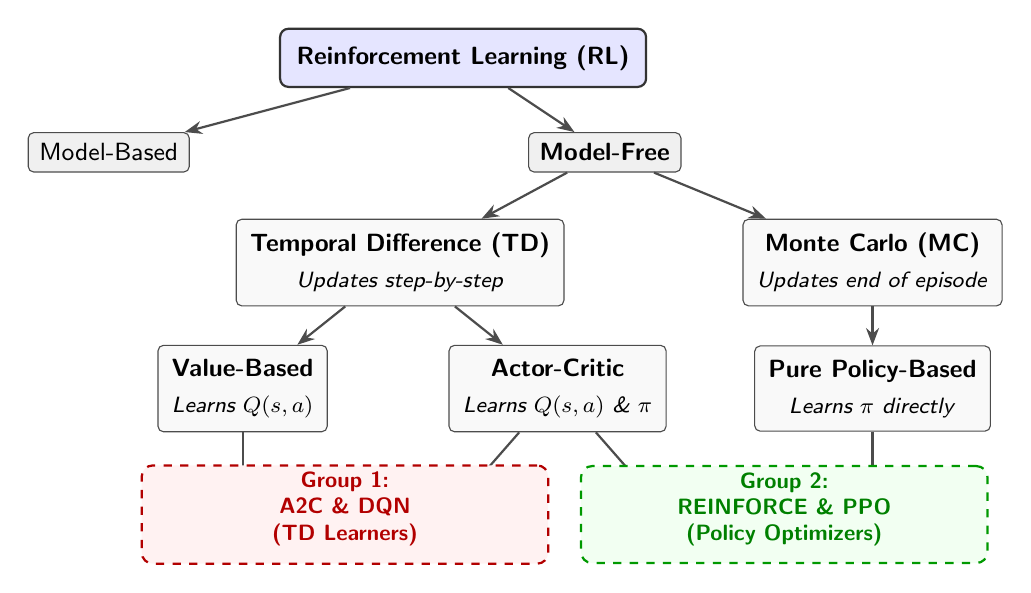
\begin{tikzpicture}[
    font=\sffamily\small,
    root/.style={rectangle, draw=black!80, fill=blue!10, thick, rounded corners=3pt, align=center, inner sep=6pt, font=\sffamily\bfseries\small},
    level1/.style={rectangle, draw=black!70, fill=gray!12, rounded corners=2pt, align=center, inner sep=4pt},
    level2/.style={rectangle, draw=black!70, fill=gray!5, rounded corners=2pt, align=center, inner sep=5pt},
    algo/.style={rectangle, draw=blue!80!black, fill=blue!10, thick, rounded corners=3pt, align=center, inner sep=5pt, font=\sffamily\bfseries\small, minimum width=1.5cm},
    group1/.style={rectangle, draw=red!70!black, fill=red!5, dashed, thick, rounded corners=4pt, inner sep=8pt},
    group2/.style={rectangle, draw=green!60!black, fill=green!5, dashed, thick, rounded corners=4pt, inner sep=8pt},
    edge_style/.style={draw=black!70, -{Stealth[length=2.2mm]}, thick}
]

% Level 0: Root
\node[root] (rl) at (0, 0) {Reinforcement Learning (RL)};

% Level 1: Model-Based / Model-Free
\node[level1] (mb) at (-4.5, -1.2) {Model-Based};
\node[level1] (mf) at (1.8, -1.2) {\textbf{Model-Free}};

% Level 2: TD / MC
\node[level2] (td) at (-0.8, -2.6) {\textbf{Temporal Difference (TD)}\\[2pt]\textit{\footnotesize Updates step-by-step}};
\node[level2] (mc) at (5.2, -2.6) {\textbf{Monte Carlo (MC)}\\[2pt]\textit{\footnotesize Updates end of episode}};

% Level 3: Paradigms
\node[level2] (vb) at (-2.8, -4.2) {\textbf{Value-Based}\\[2pt]\textit{\footnotesize Learns $Q(s,a)$}};
\node[level2] (ac) at (1.2, -4.2) {\textbf{Actor-Critic}\\[2pt]\textit{\footnotesize Learns $Q(s,a)$ \& $\pi$}};
\node[level2] (pb) at (5.2, -4.2) {\textbf{Pure Policy-Based}\\[2pt]\textit{\footnotesize Learns $\pi$ directly}};

% Level 4: Algorithm Nodes
\node[algo] (dqn) at (-2.8, -5.8) {DQN};
\node[algo] (a2c) at (-0.2, -5.8) {A2C};
\node[algo] (ppo) at (2.6, -5.8) {PPO};
\node[algo] (rf) at (5.2, -5.8) {REINFORCE};

% Connections
\draw[edge_style] (rl) -- (mb);
\draw[edge_style] (rl) -- (mf);
\draw[edge_style] (mf) -- (td);
\draw[edge_style] (mf) -- (mc);
\draw[edge_style] (td) -- (vb);
\draw[edge_style] (td) -- (ac);
\draw[edge_style] (mc) -- (pb);
\draw[edge_style] (vb) -- (dqn);
\draw[edge_style] (ac) -- (a2c);
\draw[edge_style] (ac) -- (ppo);
\draw[edge_style] (pb) -- (rf);

% Group Boxes
\node[group1, fit=(dqn) (a2c), align=center, text width=4.6cm, font=\sffamily\bfseries\footnotesize, text=red!70!black] (g1) {Group 1:\\A2C \& DQN\\(TD Learners)};
\node[group2, fit=(ppo) (rf), align=center, text width=4.6cm, font=\sffamily\bfseries\footnotesize, text=green!50!black] (g2) {Group 2:\\REINFORCE \& PPO\\(Policy Optimizers)};

\end{tikzpicture}%
}
\caption{Taxonomy tree of reinforcement learning algorithm families evaluated in this study.}
\label{fig:rl_taxonomy_tree}
\end{figure}

\begin{figure}[htbp]
\centering
\resizebox{\linewidth}{!}{%
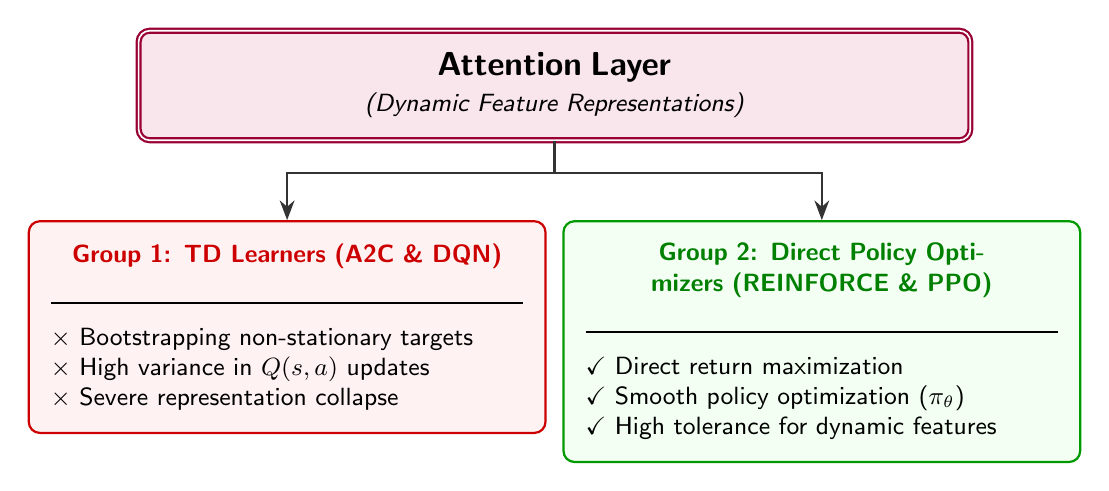
\begin{tikzpicture}[
    font=\sffamily\small,
    attn/.style={rectangle, draw=purple!80!black, fill=purple!10, double, thick, rounded corners=4pt, align=center, inner sep=8pt, text width=10cm},
    g1_box/.style={rectangle, draw=red!80!black, fill=red!5, thick, rounded corners=4pt, align=center, inner sep=8pt, text width=6cm},
    g2_box/.style={rectangle, draw=green!60!black, fill=green!5, thick, rounded corners=4pt, align=center, inner sep=8pt, text width=6cm},
    arrow/.style={draw=black!80, -{Stealth[length=2.5mm]}, thick}
]

% Top Attention Layer
\node[attn] (attn_layer) {\textbf{\large Attention Layer}\\[2pt]\textit{(Dynamic Feature Representations)}};

% Group 1 Box (Left)
\node[g1_box, below left=1.0cm and 0.1cm of attn_layer.south] (g1) {
    \textbf{\textcolor{red!80!black}{Group 1: TD Learners (A2C \& DQN)}}\\[4pt]
    \rule{\linewidth}{0.4pt}\\[4pt]
    \raggedright
    $\times$ Bootstrapping non-stationary targets\\
    $\times$ High variance in $Q(s,a)$ updates\\
    $\times$ Severe representation collapse\\
};

% Group 2 Box (Right)
\node[g2_box, below right=1.0cm and 0.1cm of attn_layer.south] (g2) {
    \textbf{\textcolor{green!50!black}{Group 2: Direct Policy Optimizers (REINFORCE \& PPO)}}\\[4pt]
    \rule{\linewidth}{0.4pt}\\[4pt]
    \raggedright
    $\checkmark$ Direct return maximization\\
    $\checkmark$ Smooth policy optimization ($\pi_\theta$)\\
    $\checkmark$ High tolerance for dynamic features\\
};

% Connections
\draw[arrow] (attn_layer.south) -- ++(0,-0.4) -| (g1.north);
\draw[arrow] (attn_layer.south) -- ++(0,-0.4) -| (g2.north);

\end{tikzpicture}%
}
\caption{Interaction model between dynamic attention layers and the two RL algorithmic taxonomy groups.}
\label{fig:rl_attention_interaction}
\end{figure}

The updated evidence motivates an architectural split between \textbf{Group 1, TD learners} (\textsc{DQN}, \textsc{A2C}), which bootstrap value estimates from a Bellman target, and \textbf{Group 2, direct policy optimizers} (\textsc{REINFORCE}, \textsc{PPO}), which use Monte-Carlo returns or clipped surrogate objectives. When dynamic attention layers sit upstream of the value network, the shifting state representation introduces non-stationarity into the bootstrapped target, destabilizing $Q$-value estimates -- explaining why \textsc{DQN} collapses toward a performance floor under attention on both schemas. Group~2 algorithms are comparatively insulated from this effect: \textsc{REINFORCE}'s un-bootstrapped full-trajectory returns and \textsc{PPO}'s trust-region clipping both tolerate shifting attention-derived features, allowing them to exploit added representational structure rather than being destabilized by it. This taxonomy directly explains the IEEE algorithm-masking effect described in Section~\ref{sec:results-ablation}.

\subsection{Why \textsc{REINFORCE} may outperform \textsc{PPO} under attention}
The taxonomy in Figure~\ref{fig:rl_taxonomy_tree} explains why Group~2 algorithms tolerate attention better than Group~1, but it does not by itself explain why \textsc{REINFORCE} overtakes \textsc{PPO} once attention is added, given that \textsc{PPO} is the stronger baseline without attention ($0.6313$ vs.\ $0.4907$ in SIT; $0.7484$ vs.\ $0.6696$ in IEEE). \textsc{PPO}'s clipped surrogate objective restricts how far a single policy update can move, which is precisely what makes it a stable, strong baseline when the observation is a plain sensor vector. However, this same clipping mechanism limits how quickly the policy can adapt once the observation itself is reshaped by an attention layer whose weights are still being learned. \textsc{REINFORCE}'s unconstrained policy-gradient updates, by contrast, allow it to adapt more rapidly to the evolving attention-derived representation, contributing to its higher peak performance once attention is present ($p=0.0007$ in SIT; $p=0.0243$ in IEEE, Table~\ref{tab:final-hyp-tests}). This suggests a complementary rather than contradictory reading of the two algorithms: \textsc{PPO} offers superior stability at baseline, while \textsc{REINFORCE} achieves a higher performance ceiling once supplied with a sufficiently informative, structured state representation.

\subsection{Implications for industrial practitioners}
Beyond the mechanistic explanation, the results translate into three practical guidelines for RL deployment in predictive maintenance:
\begin{itemize}
    \item \textbf{Avoid pooling across RL families:} Evaluating attention encoders by aggregating across value-based and policy-gradient paradigms produces misleading statistical inferences due to the algorithm masking effect documented in Section~\ref{sec:results-ablation}.
    \item \textbf{Pair attention with policy gradients:} Value-based architectures (\textsc{DQN}) are ill-suited to dynamic attention layers because of Bellman-target instability. Policy-gradient methods (\textsc{REINFORCE}, \textsc{PPO}) are a more robust default pairing.
    \item \textbf{Consider multi-head attention for stability:} If actor--critic architectures (\textsc{A2C}) must be used, multi-head attention is the most robust encoder choice, since its multi-subspace projections helped mitigate the value collapse seen with the other mechanisms.
\end{itemize}

\subsection{Why attention-style feature extraction matters---and when it does not}
The study in \cite{Siraskar2024NW} demonstrates that Nadaraya--Watson attention can represent tool-wear patterns effectively in both univariate and multivariate regression settings. That result is not itself an RL result, but it is methodologically useful because it shows that lightweight attention can extract useful structure from predictive-maintenance signals without requiring a large transformer-style architecture.

In the final RL study, attention extractor choice materially affects performance within the same algorithm, but the ablation study prevents a simplistic conclusion. Attention is not universally superior to a plain no-attention baseline. On SIT, attention is broadly helpful and especially powerful for \textsc{REINFORCE}. On IEEE, no-attention remains competitive in the pooled view, and clear attention gains emerge only for PPO and \textsc{REINFORCE}. This is one of the most important findings of the thesis because it directly addresses the research gap on schema-aware observation design.

The practical implication is that observation encoding should be treated as a selection problem rather than as a fixed modeling assumption. The most informative sensor channels, their scales, and their noise patterns differ across machines and data acquisition setups. A representation that helps on one schema can add unnecessary complexity on another. The AutoRL workflow therefore plays a dual role: it compares algorithms and also acts as a structured selection mechanism for observation encoders, including the option of using no attention at all.

\subsection{Schema portability: what is validated and what is not}
The final results show that the same environment design, reward structure, and training pipeline can be instantiated on both SIT and IEEE schemas and can yield meaningful learning and stable ranking signals on both datasets. This supports portability of the formulation and pipeline (Objective-4). It also shows that the thesis is not tied to a single handcrafted dataset pipeline.

The schema-specific choice of best mechanism is itself informative. While the reward structure and state-transition dynamics remain identical across schemas, feature complexity differs substantially. In SIT, non-parametric, distance-based attention (Nadaraya--Watson) provides the largest gain for the Monte Carlo-optimized \textsc{REINFORCE} policy ($0.8646$), consistent with a comparatively compact and homogeneous sensor set that benefits from a simple kernel-regression-style re-weighting of observations. In IEEE, the higher-dimensional, more heterogeneous force/vibration/acoustic-emission feature set instead rewards the richer projection-based transformers (self-attention and multi-head attention), pushing \textsc{REINFORCE} to $0.8860$. This indicates that the appropriate attention mechanism is itself a function of sensor-schema complexity, reinforcing why the thesis treats the encoder as a selection problem rather than a fixed choice.

However, this result must be interpreted carefully. It is not evidence that a policy trained on one schema will transfer without retraining to another schema. The thesis therefore treats schema portability as a software-and-formulation property rather than as a domain adaptation result. In other words, the method can be re-instantiated across schemas, but the policy and observation encoder still require schema-specific validation.

\subsection{Training cost versus deployment cost}
The sensitivity analysis and training-time results in \cite{Siraskar2025} highlight a practical reality: training can be slow and sensitive even for simple algorithms. For deployment-oriented use, however, training is usually performed offline on servers or workstations, while inference is the on-device requirement. The compact serialized sizes observed in the experiments suggest that inference-time storage footprint is not a primary barrier for the studied policies.

The ablation results add an important nuance. Because attention is not always superior, its extra representational complexity should be justified empirically rather than assumed. This matters for edge deployment: the best deployable model is not necessarily the most complex model, but the simplest model that achieves acceptable decision quality for the target schema. A direct energy and latency benchmark on representative edge devices is intentionally left for future work, as stated in Chapter~\ref{ch:problem-statement}.

\subsection{How the results close the literature gaps}
The literature survey identified four practical gaps: lightweight RL, schema-aware observation design, reproducible AutoRL-style experimentation, and maintenance-grounded evaluation. The results address these gaps in a connected way. First, the \textsc{REINFORCE} results show that a lightweight policy-gradient baseline deserves explicit attention in PdM rather than being omitted in favor of more complex methods. Second, the attention and no-attention comparisons show that observation design is schema-dependent and must be tested rather than assumed. Third, the AutoRL pipeline provides a reproducible mechanism for comparing algorithm--encoder combinations across repeated runs. Fourth, the final metrics evaluate replacement behavior in terms of tool usage, timing, and threshold violations, which are closer to maintenance value than raw reward totals alone.

The resulting contribution is therefore not a single model. It is a workflow: formulate the maintenance decision, instantiate the schema-specific observations, compare lightweight and deep RL learners, include no-attention as a first-class baseline, and select the algorithm--encoder pair using maintenance-grounded metrics.

\subsection{Threats to validity and limitations relevant to interpreting the results}
Several limitations matter when interpreting the reported results.
\begin{itemize}
\item \textbf{Evaluation nesting and dependence:} Repeated rounds and multiple held-out evaluations per trained model introduce dependence structure; statistical tests are therefore treated as descriptive secondary evidence.
\item \textbf{Reward and metric design:} The reported composite score reflects the selected tool-usage, timing, and violation weights. Different factories may assign different costs to early replacement, late replacement, downtime, scrap, or tool inventory.
\item \textbf{Schema-specific learning:} Both schemas are evaluated under a shared decision logic, but the thesis does not claim policy transfer across schemas.
\item \textbf{Encoder scope:} The ablation compares four attention families against a single plain baseline, but it does not exhaust the broader space of lightweight non-attention encoders that could also be competitive.
\item \textbf{Deployment validation:} Model footprint is used only as a deployment-oriented proxy; actual hardware measurements such as latency, energy use, reliability, and robustness under continuous operation are not included.
\end{itemize}


\section{Summary of key findings and objective linkage}\label{sec:results-objectives}
The results provide direct evidence for each thesis objective:
\begin{itemize}
\item \textbf{Objective-1 (environment design):} The schema-adaptive milling-tool environment supports stable training and evaluation on both SIT and IEEE, demonstrating a practical RL formulation for replacement decisions under partial observability.
\item \textbf{Objective-2 (algorithm comparison):} Across the reported protocols, \textsc{REINFORCE} is a competitive lightweight learner and is consistently stronger than \textsc{A2C} and \textsc{DQN} in the studied setup, while remaining close to or stronger than PPO depending on schema and encoder.
\item \textbf{Objective-3 (observation enhancement):} Attention-style extractors materially affect performance, but the ablation study shows that their benefit is conditional rather than universal; the best choice depends on both the observation schema and the RL algorithm, and a no-attention baseline remains an essential comparator.
\item \textbf{Objective-4 (real-world validation):} The final consolidated evaluation validates the workflow on the in-house SIT dataset and provides an external schema check on the IEEE benchmark, while avoiding a claim of direct cross-schema policy transfer.
\end{itemize}

% -------------------------------------------------------------------
% Chapter 7: Conclusions and Future Work
% -------------------------------------------------------------------

\chapter{Conclusions and Future Work}\label{ch:conclusion}

\section{Summary of the research problem and proposed solution}
This thesis investigated how reinforcement learning (RL) can be used to generate practical predictive-maintenance (PdM) decision policies for industrial milling equipment. The motivating maintenance problem is simple to state but difficult to solve: replacing a cutting tool too early wastes usable life, while replacing it too late increases the risk of poor surface quality, tool damage, rejected parts, and unplanned downtime. Traditional reactive and preventive strategies do not adapt well to changing operating conditions, and purely predictive models still require a separate decision layer to convert estimated wear or remaining useful life into action.

The literature review showed that RL-for-PdM is now a recognizable research direction, but also that several practical gaps remain. Lightweight policy-gradient methods are underrepresented; observation design is rarely validated across sensor schemas; AutoRL-style experimentation is not consistently reported; and evaluation metrics are often inconsistent across studies. The thesis therefore framed milling-tool replacement as a sequential decision problem under partial observability and developed a schema-adaptive RL workflow to address these gaps directly.

The proposed solution combines four elements: a data-driven milling-tool environment, a compact algorithm comparison including \textsc{REINFORCE}, attention and no-attention observation encoders, and a reproducible experimentation pipeline with maintenance-grounded metrics. This design moves the thesis beyond the question of whether RL can be applied to PdM. It asks which algorithm--encoder combinations are effective for a given sensor schema, and whether such policies can remain compact enough to motivate future edge-deployment studies.

\section{Fulfillment of research objectives}
Through a progression of studies---literature synthesis, preliminary algorithm evaluation, lightweight attention validation, final schema-adaptive evaluation, and matched ablation testing---the thesis addressed its four research objectives.

\paragraph{Objective-1. Design and develop an RL environment suitable for predictive maintenance:}
The thesis translated milling-tool replacement into an RL environment in which an agent observes machine-condition information, chooses whether to continue or replace, receives reward feedback, and progresses through a wear trajectory. The final environment standardizes the decision logic, threshold handling, reward structure, and evaluation outputs while allowing the observation vector to adapt to the available schema. This satisfies Objective-1 by providing a practical environment formulation for PdM under partial observability.

\paragraph{Objective-2. Evaluate RL algorithms for predictive maintenance decision making:}
The thesis evaluates \textsc{REINFORCE} alongside DQN, A2C, and PPO. The preliminary results showed that \textsc{REINFORCE} can be competitive even in untuned settings, and the final consolidated evaluation showed that it remains a strong lightweight candidate in the schema-adaptive formulation. The conclusion is not that \textsc{REINFORCE} is universally best, but that it should not be ignored in PdM settings with compact action spaces and well-defined replacement objectives.

\paragraph{Objective-3. Design, develop, and validate the core RL components – State Space, Action Space, and Reward Function:}
The thesis evaluated Nadaraya--Watson, temporal, multi-head, and self-attention encoders against matched no-attention baselines. Without attention, \textsc{PPO} gives the strongest baseline (SIT: $0.6313$; IEEE: $0.7484$). With attention, \textsc{REINFORCE} becomes the top performer (SIT: $0.8646$ with Nadaraya--Watson; IEEE: $0.8860$ with self-attention), a reversal that is statistically supported only once attention is present ($p<0.05$) and not at baseline ($p>0.90$). Value-based \textsc{DQN} showed severe degradation under attention on both schemas (an ``algorithm masking effect'' when pooled across all algorithms on IEEE), whereas policy-gradient learners leveraged attention for significant gains once isolated. Multi-head attention proved the most universally robust encoder. This satisfies Objective-3 by showing that observation enhancement must be tested against a plain baseline, and that its benefit is conditional on both algorithm family and sensor schema.

\paragraph{Objective-4. Validate the formulation on real-world milling data and a second sensor schema:}
The final evaluation used the in-house SIT milling schema as the primary real-world evidence and the IEEE PHM~2010 milling benchmark as an external schema check. The same environment logic and evaluation protocol could be instantiated on both schemas, supporting the portability of the formulation and pipeline. However, the thesis deliberately avoids claiming zero-shot policy transfer; models remain schema-specific and must be retrained and revalidated when the sensor layout changes.

\section{Practical and industrial implications}
The main practical implication is that PdM policy design should be treated as a local, schema-aware model-selection problem. A factory should not assume that a larger RL algorithm or an attention-equipped model is automatically superior. Instead, it should define the maintenance decision, construct the local observation schema, compare compact and deeper learners, include no-attention as a first-class baseline, and select the best algorithm--encoder pair using metrics that reflect replacement timing and tool usage.

The results also support a deployment-aware interpretation. Training and model selection can remain offline, while the final policy artifact can be compact enough to motivate future machine-side deployment. The small serialized sizes observed in the experiments suggest that storage footprint is unlikely to be the dominant deployment barrier for the studied policies. The remaining deployment questions are hardware-specific latency, energy use, reliability, and integration with industrial control systems.

For practitioners, the most useful takeaway is therefore procedural rather than prescriptive: do not deploy ``attention'' or ``deep RL'' as a generic label. Deploy a validated policy selected for the target machine, target sensor schema, and target maintenance objective.

\section{Limitations}
The conclusions drawn in this thesis are bounded by several structural limitations:
\begin{itemize}
\item \textbf{Schema dependence and transferability:} The results validate a schema-adaptive workflow, not direct transfer of trained policies across sensor schemas. A model trained on one machine or schema should be retrained and revalidated when the sensing layout changes substantially.
\item \textbf{Reward scaling and economic generalization:} The composite score reflects the selected tool-usage, timing, and violation weights. Different factories may assign different costs to early replacement, late replacement, downtime, scrap, or tool inventory.
\item \textbf{Training cost versus inference cost:} The final policies are compact at inference time, but training and repeated model selection still require offline computational effort.
\item \textbf{On-device metrics:} Deployment feasibility is inferred only indirectly through model size and decision simplicity. Direct hardware measurements such as latency, energy use, reliability, and robustness under continuous operation are not included.
\item \textbf{Encoder search scope:} The ablation compares four attention families against a plain baseline, but it does not exhaust the wider space of lightweight non-attention encoders that may also be competitive.
\item \textbf{Evaluation dependence:} Repeated evaluations and stochastic policy behavior introduce dependence structures, so the statistical tests are treated as descriptive support rather than as the sole basis for inference.
\end{itemize}

\section{Future work}
Based on the defined limitations and findings, the following avenues are proposed for future research:
\begin{itemize}
\item \textbf{Domain Adaptation and Few-Shot Learning:} Researchers should investigate methods to initialize target-schema policies from source-schema weights. Transferring learned representations across different cutting regimes or materials could reduce the data volume required for a new machine tool.
\item \textbf{Hardware-in-the-Loop Edge Evaluation:} Follow-on research should run cycle-accurate latency, reliability, and power tests by executing derived policies on industrial programmable logic controllers (PLCs) or edge accelerators such as Raspberry Pi or NVIDIA Jetson devices, with particular attention to the inference latency and memory bandwidth of multi-head attention blocks, since multi-head attention emerged as the most universally robust encoder in this study.
\item \textbf{Multi-Objective AutoRL Search:} The AutoRL pipeline could be formalized to treat deployment cost, parameter count, memory footprint, and policy precision as a Pareto-optimal search problem rather than as separate reporting dimensions.
\item \textbf{Broader Observation Encoder Search:} Future studies should expand the search space beyond the current attention families and plain baseline to include other lightweight feature encoders, enabling a more complete assessment of when attention is genuinely advantageous.
\item \textbf{Continuous Learning under Concept Drift:} Real factories observe gradual tool-degradation shifts across seasons, materials, operators, and cutting regimes. Designing RL agents that safely support online adaptation or human-in-the-loop override is therefore a necessary step toward autonomous shop-floor execution.
\end{itemize}

\section{Final remarks}
This thesis shows that carefully designed, lightweight reinforcement learning models, paired with empirically validated observation encoders, provide a feasible path for predictive maintenance in milling-tool replacement. Its central contribution is not merely a high-performing policy, but a reproducible decision workflow that links literature gaps to environment design, schema-aware observation handling, algorithm comparison, ablation testing, and maintenance-grounded evaluation. The work therefore moves RL-driven PdM closer to practical factory use while preserving an important caution: every deployment must be validated against the target machine, sensor schema, and maintenance objective.

\bibliographystyle{plainnat}
\bibliography{thesis-bliography}

\end{document}

